% main_co2_nature_20260903.tex  (five-layer restructure after LZ comments, 2026-09-03)
% Built from main_co2_nature_20260826.tex (preserved) by 27_assemble_tex.py, which
% inserts the generated table fragments (_tex_*.tex) at the %%TAB_*%% markers.
% Layers (LZ): 1 causal effect (country 2SLS + airport evidence), 2 mechanism
% (identity decomposition), 3 heterogeneity, 4 spillovers (own and neighbour
% connectivity jointly instrumented), 5 policy. Methods gains the decomposition
% identity, the airport design and pilot, the spillover design, and the
% exclusion-restriction diagnostics. Corrections relative to 08-26: the
% heterogeneity results now use TOTAL CO2 (the 08-26 numbers 11.43/5.91/0.35 were
% the international-CO2 outcome mislabelled as total); the inverse-distance
% spillover (7.45) is retained only as a reference row because it is fragile
% under country clustering and a permutation placebo; the headline spillover is
% the contiguity specification with own and neighbour connectivity jointly
% instrumented. Display count is above Nature limits; at submission move
% Tables decomp/spillover or Figures to Extended Data as the editor requires.
\documentclass[12pt]{article}
\usepackage[margin=2.2cm]{geometry}
\usepackage{amsmath,graphicx,booktabs,threeparttable,float}
\title{How Much Does Air Connectivity Increase Aviation CO$_2$?}
\author{[author order TBD]}
\date{Nature-format draft, 3 September 2026}
\begin{document}
\maketitle

\begin{abstract}
\noindent Air connectivity is an explicit object of national policy, yet its
carbon consequences have never been estimated causally at the global level.
Here we construct flight-stage-resolved CO$_2$ for more than 6{,}000
airports over 1996--2023 from schedule data, match it to a global panel of
airport connectivity, and identify the effect of connectivity on emissions
with an instrument based on each country's air-versus-sea market-access
geography. A one percent increase in connectivity raises national aviation
CO$_2$ by 5.7 percent, an elasticity far above one and invariant to how
emissions are allocated across countries. Decomposing the response on the
accounting identity shows that it is a frequency response: flights rise by
7.0 percent, aircraft size and stage length do not rise, and the 0.4 percent
decline in emissions per seat-kilometre offsets seven percent of the scale
effect. The elasticity is concentrated in low-income, newly connecting
countries and describes the take-off stage of network development, in
level as well as in logarithmic specifications; at the airport level it is systemic rather than hub-driven,
although the emissions it generates are more concentrated than emissions
themselves and are led by new hubs. Emissions also respond to the
connectivity of contiguous neighbours, with an elasticity of 1.9 when own and
neighbour connectivity are jointly instrumented. Connectivity growth since
1996 accounts for 42.5 percent (356 Mt) of 2023 aviation CO$_2$, an annual
external cost of \$18 billion to \$68 billion at standard social-cost-of-carbon
values, and only sustained fuel switching, not the efficiency gains of
network development, materially lowers this level.
\end{abstract}

%=======================================================================
\section*{Main [Yifu]}
%=======================================================================
Air connectivity is an explicit object of national policy. Governments
subsidise routes, expand airport capacity, and negotiate air-service
agreements on the premise that connections to the global air network raise
trade, tourism, and productivity, and a large literature documents such
gains [TODO cite]. Aviation is also among the most difficult transport
sectors to decarbonise: it has no near-term electrification path, and its
emissions are governed by separate international accounting conventions
rather than by national inventories [TODO cite]. The carbon consequences of
connectivity policy are therefore a first-order question, and one for
which, to our knowledge, no causal estimate exists at the global level.

The direction of the effect is not in serious doubt: more connections mean
more flying. The empirical questions concern magnitude and structure.
First, proportionality: does a one percent gain in connectivity raise
emissions by more or less than one percent, and through which margin of
aviation activity? Network development changes not only the amount of
flying but its organisation, since hub formation can consolidate traffic
into fewer, fuller, and more efficient movements. Second, incidence: which
countries and which airports carry the response, and does it spill across
borders through the network? Third, accounting: the emissions generated by
connectivity growth need not be booked where they are generated, because
international aviation is attributed under bunker conventions rather than
territorially [TODO cite].

We answer these questions with two inputs (Methods). The first is a new
emissions panel: flight-stage-resolved CO$_2$ computed from OAG schedule
data under the EEA/EMEP Guidebook methodology for 6{,}356 airports over
1996--2023, disaggregated by flight stage and by domestic and international
traffic, so that national emissions can be constructed under any allocation
rule without double counting and so that the response can be decomposed on
the identity used to build the data. The second is identification: we
instrument a country's connectivity, measured by the Global Air
Connectivity Index (GACI), with the interaction of world aviation
technology and the country's air-versus-sea market-access geography in
1996, in the spirit of Feyrer [TODO cite]. The instrument is strong
(first-stage Kleibergen--Paap $F = 154$), survives a stress test that
interacts the global cycle with baseline population, income, and airport
capacity, and passes a battery of exclusion-restriction diagnostics that we
report in full, including the cases in which the identifying variation
cannot be separated from rival global cycles (Methods). The analysis is
organised in five layers: the causal effect at the country and airport
levels, its decomposition on the accounting identity, its heterogeneity,
its cross-border spillovers, and its policy accounting.

%=======================================================================
\section*{Results [Sunbin]}
%=======================================================================
\subsection*{The emissions elasticity of connectivity is far above one}
Table~\ref{tab:main} reports the central result. Because the question is
whether connectivity growth raises emissions more or less than
proportionally, the relevant benchmark is an elasticity of one. The
two-stage least squares estimate is far above it: a one percent increase in
connectivity raises total bunker CO$_2$ by 5.67 percent (s.e.\ 0.41), and
the hypothesis that the elasticity equals one is rejected at any
conventional level. The estimate is insensitive to how emissions are
assigned to countries, ranging from 5.62 under a 50/50 split of cruise
emissions to 5.92 under the territorial rule, and it is stable across
aggregations of airport connectivity to the country level
(Table~\ref{tab:main}, Panels C--E). Ordinary least squares estimates are
roughly forty percent smaller, consistent with attenuation from measurement
error in the connectivity index. The identifying variation is present in
both halves of the sample once crisis years are set aside: the elasticity
is 5.61 (s.e.\ 0.66) for 1996--2007 and 3.01 (s.e.\ 0.64) for 2010--2023
excluding the COVID-19 collapse, so it declines by roughly half between the
network-expansion and the mature-network eras ($p = 0.005$) but remains far
above one in both (Extended Data Table~\ref{tab:temporal} and Extended Data
Fig.~\ref{fig:temporal}). The estimate is also robust to inference: with
standard errors clustered by country the $t$-statistic is 5.1, and the
elasticity moves within 4.7 to 4.9 when log GDP, trade openness,
urbanisation, foreign direct investment and tourist arrivals are added as
controls, although these are outcomes of connectivity themselves
(Extended Data Table~\ref{tab:exclusion}).

The same variation raises seat-kilometres by 6.07 percent, faster than
emissions, so emissions per seat-km fall by 0.40 percent
(Table~\ref{tab:main}, column 6). An efficiency margin therefore exists,
but it offsets a small fraction of the scale response, a point we quantify
below.

\begin{table}[htbp]
\centering
\begin{threeparttable}
\caption{Air connectivity and aviation CO$_2$: main results}
\label{tab:main}
\footnotesize
\begin{tabular}{lcccccc}
\toprule
 & \multicolumn{1}{c}{Bunker CO$_2$} & \multicolumn{1}{c}{LTO CO$_2$} & \multicolumn{1}{c}{50/50 CO$_2$} & \multicolumn{1}{c}{Intl.\ CO$_2$} & \multicolumn{1}{c}{Seat-km} & \multicolumn{1}{c}{Intensity} \\
 & (1) & (2) & (3) & (4) & (5) & (6) \\
\midrule
\multicolumn{7}{l}{\textit{Panel A. OLS}} \\
  ln GACI (cwm) & 3.585$^{***}$ & 3.043$^{***}$ & 3.566$^{***}$ & 3.874$^{***}$ & 3.941$^{***}$ & -0.355$^{***}$ \\
   & (0.175) & (0.177) & (0.175) & (0.198) & (0.183) & (0.043) \\
  $N$ & 4,634 & 4,634 & 4,634 & 4,633 & 4,634 & 4,634 \\
\midrule
\multicolumn{7}{l}{\textit{Panel B. 2SLS, Feyrer instrument, capacity-weighted mean}} \\
  ln GACI (cwm) & 5.669$^{***}$ & 5.921$^{***}$ & 5.620$^{***}$ & 5.690$^{***}$ & 6.068$^{***}$ & -0.399$^{***}$ \\
   & (0.412) & (0.448) & (0.409) & (0.415) & (0.443) & (0.118) \\
  KP $F$ & 153.6 & 153.6 & 153.6 & 152.7 & 153.6 & 153.6 \\
  $N$ & 4,634 & 4,634 & 4,634 & 4,633 & 4,634 & 4,634 \\
\midrule
\multicolumn{7}{l}{\textit{Panel C. 2SLS, GACI sum}} \\
  ln GACI (sum) & 2.283$^{***}$ & 2.384$^{***}$ & 2.263$^{***}$ & 2.291$^{***}$ & 2.443$^{***}$ & -0.161$^{***}$ \\
   & (0.224) & (0.219) & (0.222) & (0.237) & (0.250) & (0.052) \\
  KP $F$ & 90.3 & 90.3 & 90.3 & 89.5 & 90.3 & 90.3 \\
  $N$ & 4,634 & 4,634 & 4,634 & 4,633 & 4,634 & 4,634 \\
\midrule
\multicolumn{7}{l}{\textit{Panel D. 2SLS, GACI max}} \\
  ln GACI (max) & 4.822$^{***}$ & 5.036$^{***}$ & 4.780$^{***}$ & 4.836$^{***}$ & 5.161$^{***}$ & -0.340$^{***}$ \\
   & (0.329) & (0.348) & (0.327) & (0.343) & (0.361) & (0.101) \\
  KP $F$ & 172.0 & 172.0 & 172.0 & 171.0 & 172.0 & 172.0 \\
  $N$ & 4,634 & 4,634 & 4,634 & 4,633 & 4,634 & 4,634 \\
\midrule
\multicolumn{7}{l}{\textit{Panel E. 2SLS, GACI mean}} \\
  ln GACI (mean) & 5.897$^{***}$ & 6.159$^{***}$ & 5.846$^{***}$ & 5.902$^{***}$ & 6.313$^{***}$ & -0.415$^{***}$ \\
   & (0.591) & (0.623) & (0.587) & (0.593) & (0.624) & (0.122) \\
  KP $F$ & 136.2 & 136.2 & 136.2 & 135.6 & 136.2 & 136.2 \\
  $N$ & 4,634 & 4,634 & 4,634 & 4,633 & 4,634 & 4,634 \\
\bottomrule
\end{tabular}
\begin{tablenotes}[flushleft]
\footnotesize
\item Notes: Country-year panel, 1996--2023. All specifications include country and year fixed effects and control for log population and log sea market access. Outcomes are in logs: total aviation CO$_2$ under the bunker convention (all cruise plus departure-side LTO assigned to the departure country), landing-and-take-off CO$_2$ only, CO$_2$ with cruise split 50/50 between endpoint countries, bunker CO$_2$ from international flights, scheduled departing seat-kilometres, and CO$_2$ per seat-km. The instrument in Panels B--E interacts world aviation technology with air-versus-sea geography (Feyrer-type). Robust standard errors in parentheses. $^{***}$, $^{**}$, $^{*}$: significance at 1, 5, and 10 percent.
\end{tablenotes}
\end{threeparttable}
\end{table}

\subsection*{Airport-level evidence: the response is systemic, and its
emissions are led by new hubs}
The country estimates could in principle be an artefact of national
aggregation, with a few hubs carrying the aggregate. The airport panel
(5{,}354 airports that are nodes of the connectivity network, 97{,}165
airport-years) allows a within-country test. With airport and
country-by-year fixed effects, so that every national shock is absorbed and
airports are compared with other airports of the same country in the same
year, a one percent increase in an airport's connectivity is associated
with 3.72 percent more CO$_2$, 4.18 percent more seat-kilometres, a 0.49
percent decline in CO$_2$ per seat-km and a 0.33 percentage point higher
international share (Extended Data Table~\ref{tab:airport_het}). These
estimates are descriptive: the airport-level Feyrer shifter we piloted has
no first stage within countries, and an earlier heritage-proximity pilot
failed the size-by-cycle test, so no valid airport-level instrument is
available (Methods; Supplementary Table~\ref{tab:airport_iv}).

The within-country elasticity is not hub-driven. It is 2.0 to 2.1 at the
airports that were in the global top one or five percent by 1996 capacity
and 3.8 to 4.0 elsewhere, and the pooled interaction of hub status with
connectivity is $-2.56$ (s.e.\ 0.20). It is highest in the middle tercile
of baseline connectivity (5.85, against 4.18 in the bottom and 2.90 in the
top tercile), at domestically oriented and at highly international airports
alike (4.24 and 4.69), in Africa (6.03) and Europe (4.45), and lowest in
North America (2.59). Because airport GACI embeds a capacity term, we
re-estimate with the topology-only components of the index; closeness
centrality reproduces the pattern (4.41 on CO$_2$, $-0.70$ on intensity),
and every component lowers intensity. At the node, therefore, connectivity
growth raises emissions broadly across the network, and the efficiency
margin is real: the cross-sectional efficiency curve in
Fig.~\ref{fig:effcurve} shows median intensity falling monotonically from
284 to 77 kg per 1{,}000 seat-km across connectivity ventiles while the
international share rises from one to sixty percent.

A systemic elasticity does not imply a dispersed emissions consequence,
because the elasticity multiplies very unequal bases. Applying the country
elasticity to each airport's connectivity change since 1996 attributes 345
Mt of 2023 emissions to connectivity growth across airports, consistent
with the 356 Mt country total, and the attributed emissions are more
concentrated than emissions themselves: the top one percent of airports
hold 45.8 percent of the attributed total against 41.0 percent of
emissions, the top five percent hold 84.5 against 77.6 percent, and the
Gini coefficient is 0.945 against 0.916 (Fig.~\ref{fig:airportconc} and
Table~\ref{tab:airport_conc}). The concentration is not in the incumbent
hubs: the 260 airports in the 1996 global top five percent hold 68.5
percent of the attributed total against 75.3 percent of emissions, and the
largest single contributions are Dubai (19.4 Mt), Doha (12.3), Shanghai
Pudong (11.2), Istanbul (10.3) and Incheon (9.9). The climate consequence
of connectivity growth is thus generated throughout the network but
accumulates at the hubs that the growth created.

\begin{figure}[htbp]
\centering
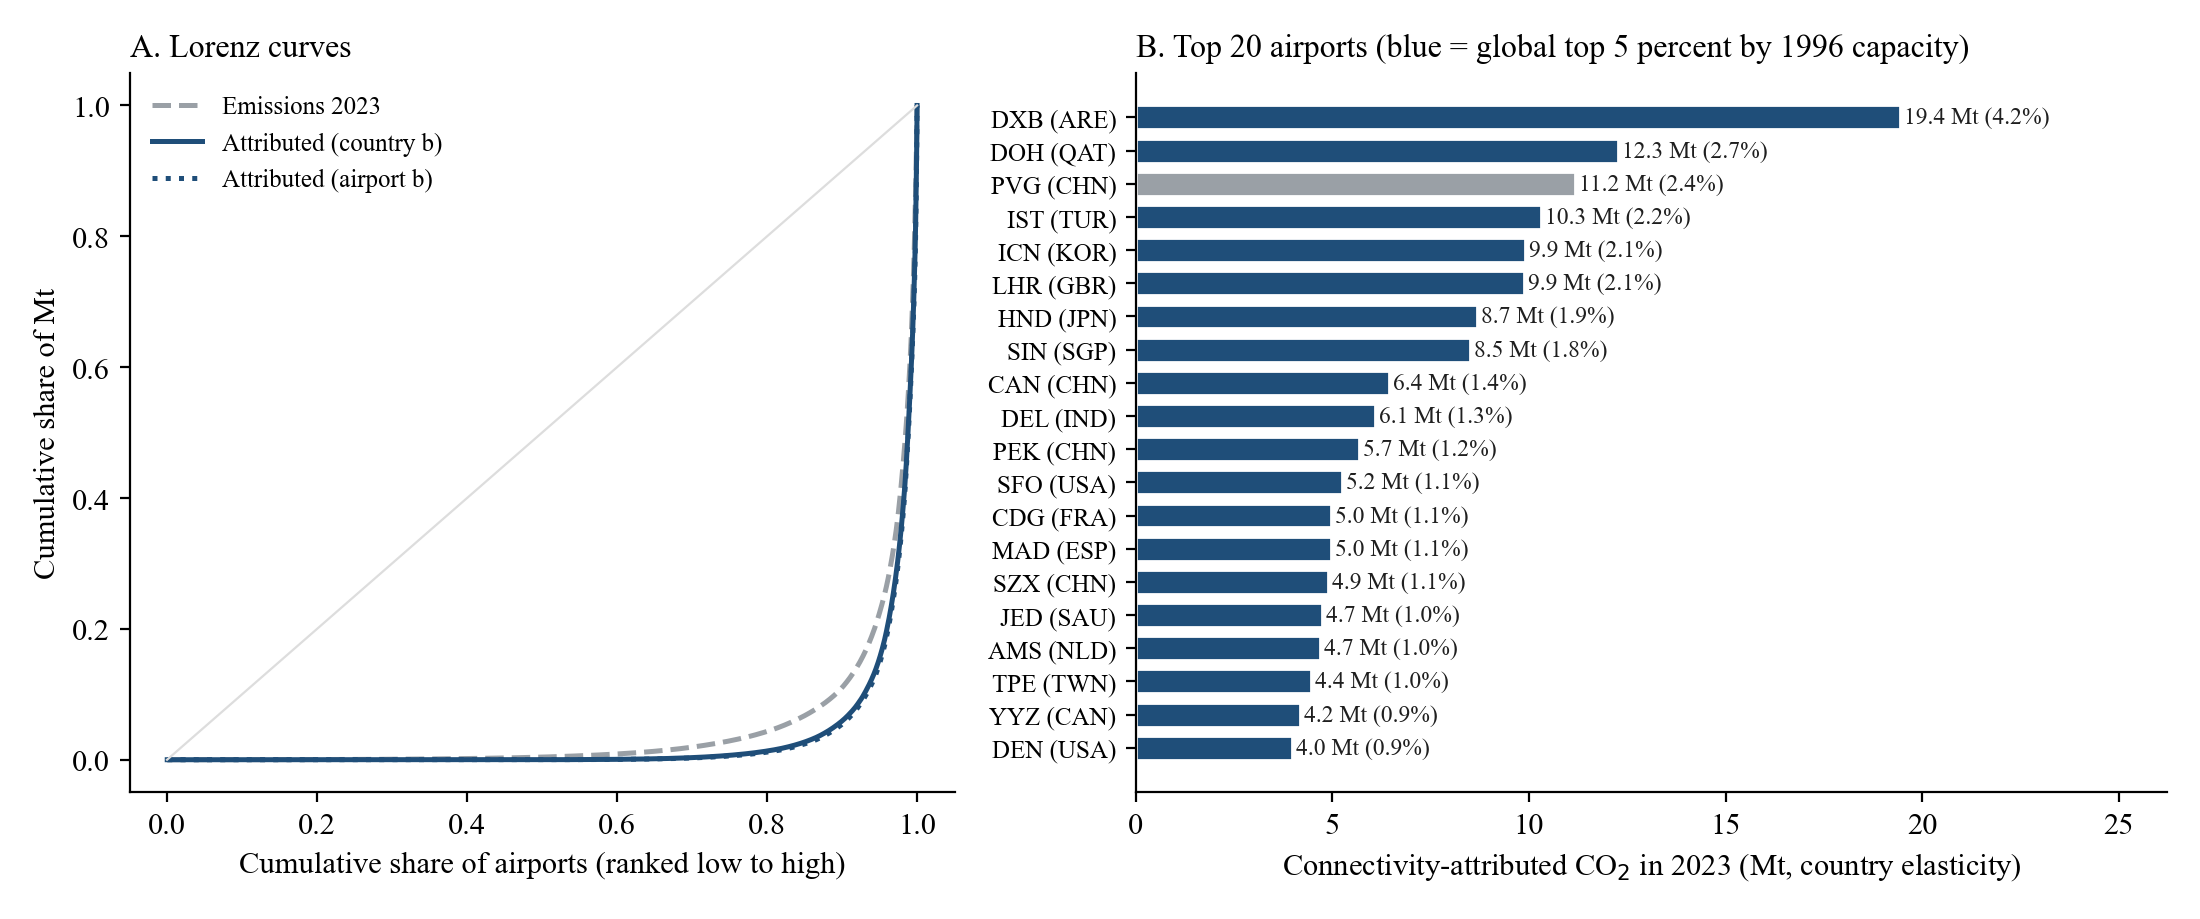
\includegraphics[width=0.98\textwidth]{CO2_airport_concentration.png}
\caption{\textbf{Concentration of connectivity-attributed emissions across airports, 2023.} A, Lorenz curves of 2023 emissions and of emissions attributed to 1996--2023 connectivity growth over 3{,}833 airports with positive emissions. B, the twenty largest attributed contributions (Mt and share of the world attributed total); blue marks airports in the global top five percent by 1996 capacity.}
\label{fig:airportconc}
\end{figure}

\begin{table}[htbp]
\centering
\begin{threeparttable}
\caption{Concentration of connectivity-attributed emissions across airports, 2023}
\label{tab:airport_conc}
\footnotesize
\begin{tabular}{lccccc}
\toprule
 & Top 1\% & Top 5\% & Top 10\% & Top 25\% & Gini \\
\midrule
  Emissions 2023 & 41.0 & 77.6 & 89.0 & 97.1 & 0.916 \\
  Attributed (country b) & 45.8 & 84.5 & 94.1 & 99.3 & 0.945 \\
  Attributed (airport b) & 46.8 & 85.3 & 94.6 & 99.4 & 0.948 \\
  Attributed (hub/non-hub b) & 45.0 & 82.8 & 93.3 & 99.3 & 0.941 \\
\bottomrule
\end{tabular}
\begin{tablenotes}\footnotesize
\item Shares (percent) of the global total held by the top-ranked airports, and Gini coefficients, over the 3,833 airports with positive 2023 emissions. Attributed emissions are CO$_2$ in 2023 times $1-\exp(-\beta\,\Delta\ln \mathrm{GACI}_{1996\text{--}2023})$ with $\beta$ from the country 2SLS (5.67), the airport within-country regression (3.72), or the hub-specific airport estimates (2.11 for the global top 5 percent by 1996 capacity, 4.05 otherwise). Negative attributions (airports whose connectivity fell) are set to zero in the ranking.
\end{tablenotes}
\end{threeparttable}
\end{table}

\begin{figure}[htbp]
\centering
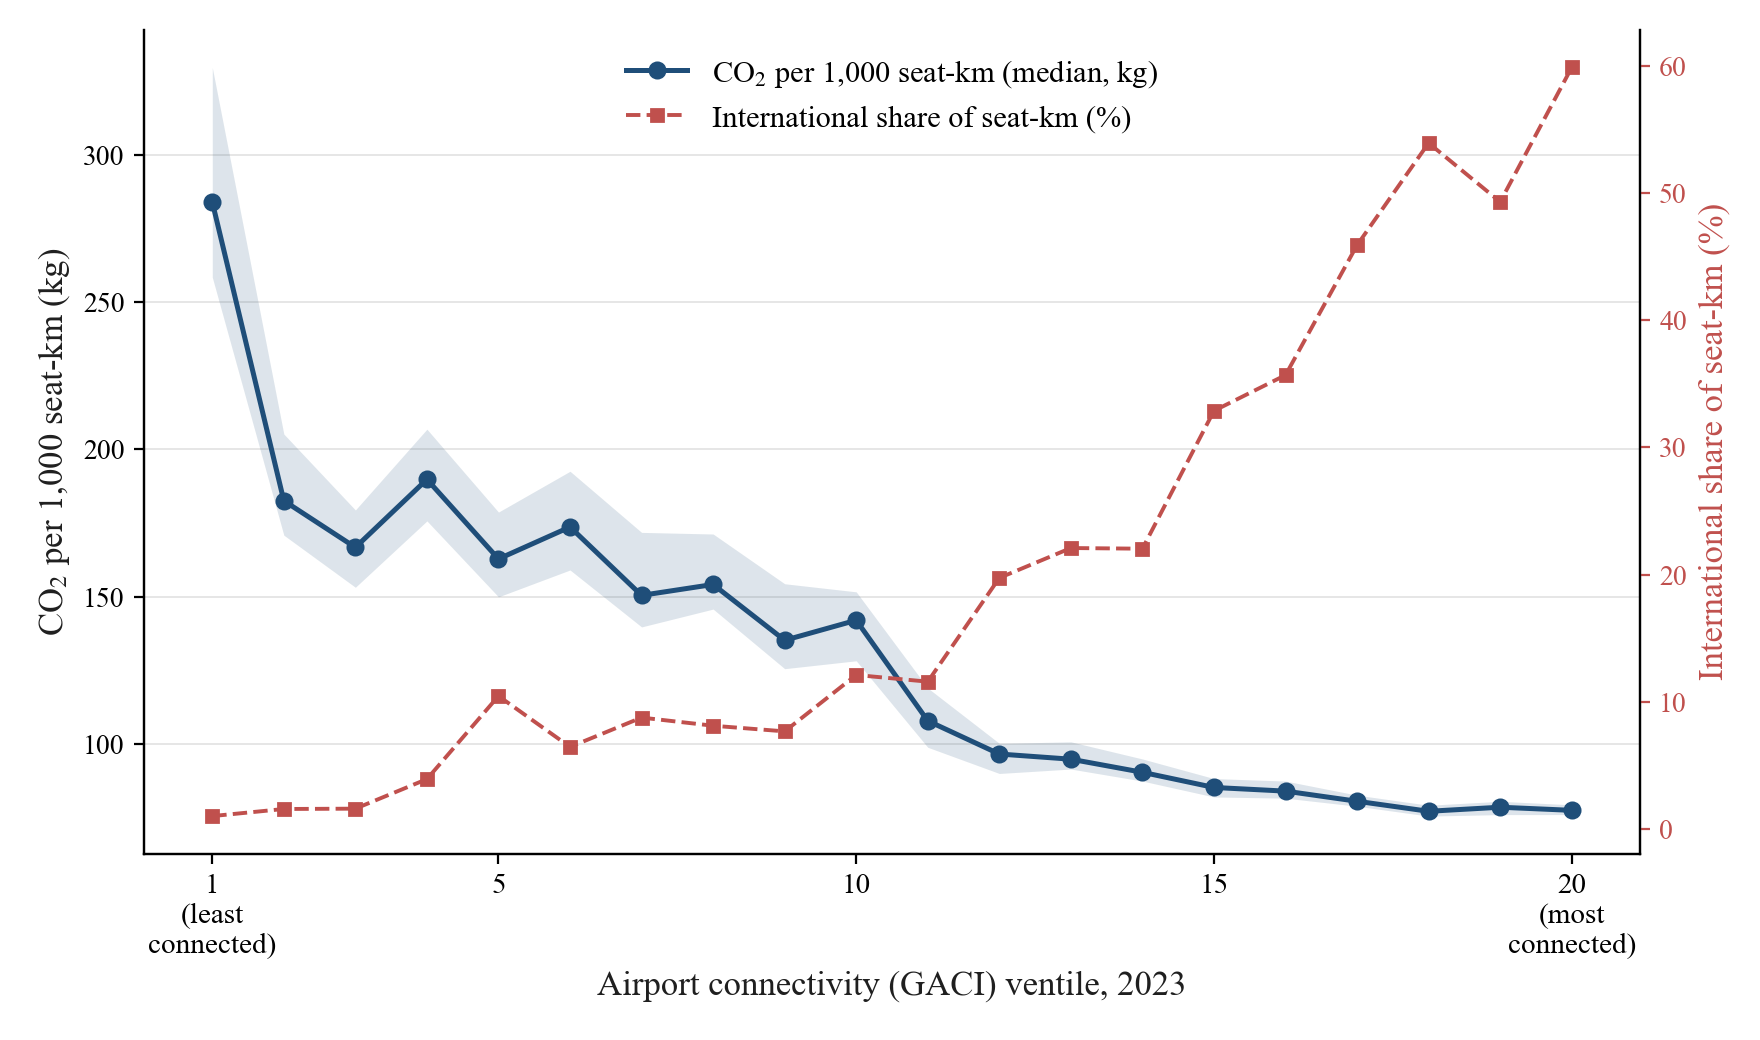
\includegraphics[width=0.92\textwidth]{CO2_efficiency_curve.png}
\caption{\textbf{Airport-level efficiency curve, 2023:} median kg CO$_2$ per 1{,}000 seat-km by connectivity ventile, with the international share of seat-km on the second panel.}
\label{fig:effcurve}
\end{figure}

\subsection*{Where the elasticity comes from: frequency, not aircraft size
or efficiency}
An elasticity of 5.67 invites the question of its origin. Because the
emissions data are built from scheduled flights, national CO$_2$ is
exactly the product of flights, seats per flight, kilometres per flight and
CO$_2$ per seat-kilometre (Methods, equation~\ref{eq:identity}), so the
log elasticities of the four components with respect to connectivity add
to the total (equation~\ref{eq:decomp}). Table~\ref{tab:decomp} and
Fig.~\ref{fig:waterfall} report the decomposition on the identical sample.
The response is a pure frequency response: flights rise by 6.98 percent for
a one percent gain in connectivity, aircraft gauge does not change
($-0.30$, s.e.\ 0.23), stage length shortens slightly ($-0.60$), and
emissions per seat-km fall by 0.40 percent. Scale, the sum of the first
three terms, contributes 6.07 or 107 percent of the total; the efficiency
term offsets seven percent of it, so the traffic expansion outweighs the
efficiency gain by a factor of fifteen. The composition margins are small:
the share of landing-and-take-off emissions does not move and the
international share of seat-km rises by 0.1 percentage point. Causal
mediation on the same data (Extended Data Table~\ref{tab:mediation})
attributes 84 to 87 percent of the total effect to flight frequency and
seat-kilometres, and essentially nothing to the international share.

\begin{table}[htbp]
\centering
\begin{threeparttable}
\caption{Decomposition of the CO$_2$ elasticity on the accounting identity}
\label{tab:decomp}
\footnotesize
\begin{tabular}{lccc}
\toprule
 & Elasticity to GACI & s.e. & Share of total (\%) \\
\midrule
\multicolumn{4}{l}{\textit{Scale components}} \\
  Flights (frequency) & +6.976$^{***}$ & (0.570) & +123 \\
  Seats per flight (aircraft gauge) & -0.303 & (0.226) & -5 \\
  Km per flight (average stage length) & -0.605$^{***}$ & (0.211) & -11 \\
  \textbf{Subtotal: scale (seat-km)} & +6.068$^{***}$ & (0.443) & +107 \\
\multicolumn{4}{l}{\textit{Efficiency component}} \\
  CO$_2$ per seat-km (carbon intensity) & -0.399$^{***}$ & (0.118) & -7 \\
\midrule
  \textbf{Total CO$_2$ (equals Table~\ref{tab:main}, column 1)} & +5.669$^{***}$ & (0.412) & +100 \\
\midrule
\multicolumn{4}{l}{\textit{Composition margins (memo)}} \\
  LTO share of CO$_2$ & +0.014 & (0.025) & -- \\
  International share of seat-km & +0.096$^{**}$ & (0.048) & -- \\
\bottomrule
\end{tabular}
\begin{tablenotes}\footnotesize
\item Each row is a separate 2SLS regression of the log component on log GACI (capacity-weighted mean), instrumented by the Feyrer interaction, with log population and log sea market access, country and year fixed effects, and heteroskedasticity-robust standard errors; identical sample of 4,634 country-years, first-stage Kleibergen-Paap $F$ = 153.6. Because CO$_2$ = flights $\times$ seats per flight $\times$ km per flight $\times$ CO$_2$ per seat-km, the log elasticities add exactly to the total. Load factor is constant by construction (scheduled capacity) and cancels. Shares are component elasticity divided by the total. $^{***}$ $p<0.01$, $^{**}$ $p<0.05$, $^{*}$ $p<0.1$.
\end{tablenotes}
\end{threeparttable}
\end{table}

\begin{figure}[htbp]
\centering
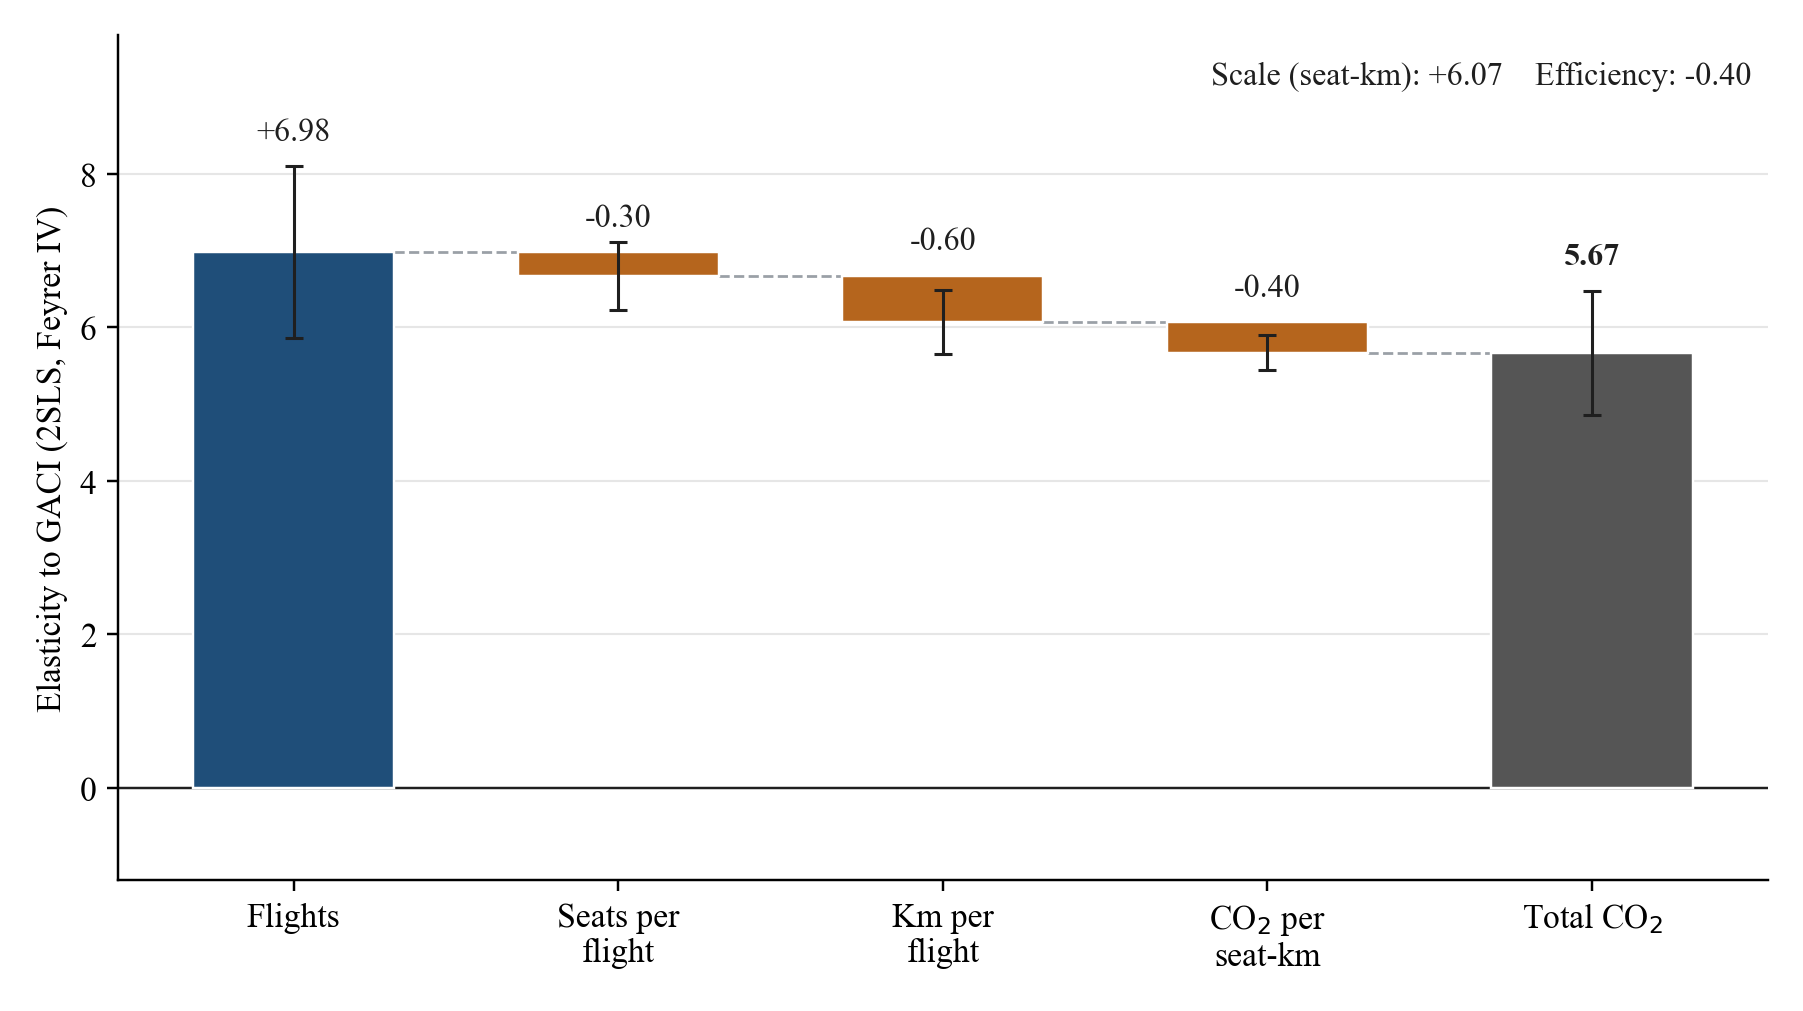
\includegraphics[width=0.85\textwidth]{CO2_decomp_waterfall.png}
\caption{\textbf{Decomposition of the CO$_2$ elasticity on the accounting identity.} Each bar is the 2SLS elasticity of the component with respect to connectivity (Feyrer instrument; 95 percent confidence intervals); the components add exactly to the total. Scale is the sum of the first three bars.}
\label{fig:waterfall}
\end{figure}

The decomposition also explains why the elasticity differs so much across
countries (Extended Data Table~\ref{tab:decomp_hetero}). In the bottom
income tercile every scale margin expands, flights by 8.8 percent, aircraft
size by 0.9 and stage length by 1.7, and intensity falls by 1.1 percent,
giving a total of 10.4. In the middle tercile flights rise by 8.6 percent
but stages shorten by 1.7, giving 6.1. In the top tercile flights still
rise (8.5, s.e.\ 2.9) but aircraft become smaller ($-3.3$) and stages
shorter ($-4.3$), and intensity does not improve, so the total is 1.8 and
imprecise: in mature networks connectivity growth adds short, thin
frequencies whose emissions are largely offset by the reorganisation of
the existing traffic. Applying the identity separately to international
and domestic departures shows that the international elasticity (5.69) is
carried by frequency (6.03) with a small up-gauging (0.58) and the largest
intensity gain ($-0.52$), while domestic emissions do not respond
($-0.64$, s.e.\ 1.14). A secondary instrument whose compliers are
hub-quality changes rather than market-access growth points to the same
composition margin: under it, total emissions do not respond, but
international emissions rise by 3.16 percent and emissions per seat-km by
1.23 percent (Methods).

\subsection*{The elasticity is concentrated in newly connecting countries}
The world average combines countries entering the network with countries
already saturated. Splitting the sample by 1996 characteristics yields a
steep gradient (Fig.~\ref{fig:hetero} and Extended Data
Table~\ref{tab:hetero}): the elasticity of total CO$_2$ is 10.40 (s.e.\
1.22) in the bottom income tercile, 6.14 in the middle and 1.83 (s.e.\
0.97, $p = 0.06$) at the top, and the pooled interaction of the top tercile
with connectivity is $-3.33$ (s.e.\ 0.23). By baseline connectivity the
elasticity falls from 8.46 in the bottom tercile to 5.07 in the middle; the
top tercile has too weak a first stage ($F = 1.8$) for inference, a fact we
use below as a diagnostic. Regionally, the elasticity is 6.36 in Africa,
5.33 in Asia--Pacific and 2.92 in Latin America, while Europe is a
precisely estimated zero ($-0.61$, s.e.\ 0.64). The efficiency margin
follows the same geography: emissions per seat-km fall significantly only
in the bottom income tercile. The headline elasticity therefore describes
the network's extensive margin; for mature networks, connectivity growth is
approximately carbon-neutral at the margin, for the reason the
decomposition makes explicit.

\subsection*{What the elasticity represents: the take-off stage of network
development}
Three further results fix the interpretation of the headline number. First,
the gradient is not an artefact of the logarithmic scale. A country whose
index rises from a very low base records a large percentage change for a
small absolute addition, so we re-estimate the relationship with
connectivity in levels (Extended Data Table~\ref{tab:funcform}). The
semi-log slope is 4.09 log points of CO$_2$ per unit of GACI (s.e.\ 0.35),
an elasticity of 4.4 at the sample mean, and the level-level slope is 4.2
Mt per unit; within baseline-connectivity terciles the semi-log slope is
10.3 in the bottom tercile, 4.6 in the middle and 1.1 (s.e.\ 0.6) at the
top, so the same absolute addition to the network raises emissions far
more where the network is thin. Second, the gradient is a step rather than
a smooth slope, and it is not confined to the very bottom of the
distribution (Fig.~\ref{fig:gradient} and Extended Data
Table~\ref{tab:gradient}). Quintile splits give elasticities of 8.5 in
both of the two lowest quintiles, 3.3 in the third and 4.1 in the fifth,
while the fourth is unidentified; a pooled specification that interacts
connectivity with centred log baseline connectivity, with the instrument
interacted identically, gives a fitted elasticity of 7.1 at the tenth
percentile of baseline connectivity, 6.0 at the median and 4.1 at the
ninetieth, with the quadratic term indicating a floor rather than a
continued decline. Third, the identifying variation is itself
concentrated in the expansion era: the first stage is strong before 2010
and in the mature era only once the COVID years are excluded, and the
elasticity falls from 5.6 to 3.0 across the two eras. The headline
elasticity is therefore best read as the emissions response during the
take-off stage of national network development, which the sample
observes for most countries between 1996 and the late 2000s, and not as a
universal constant.

\begin{figure}[htbp]
\centering
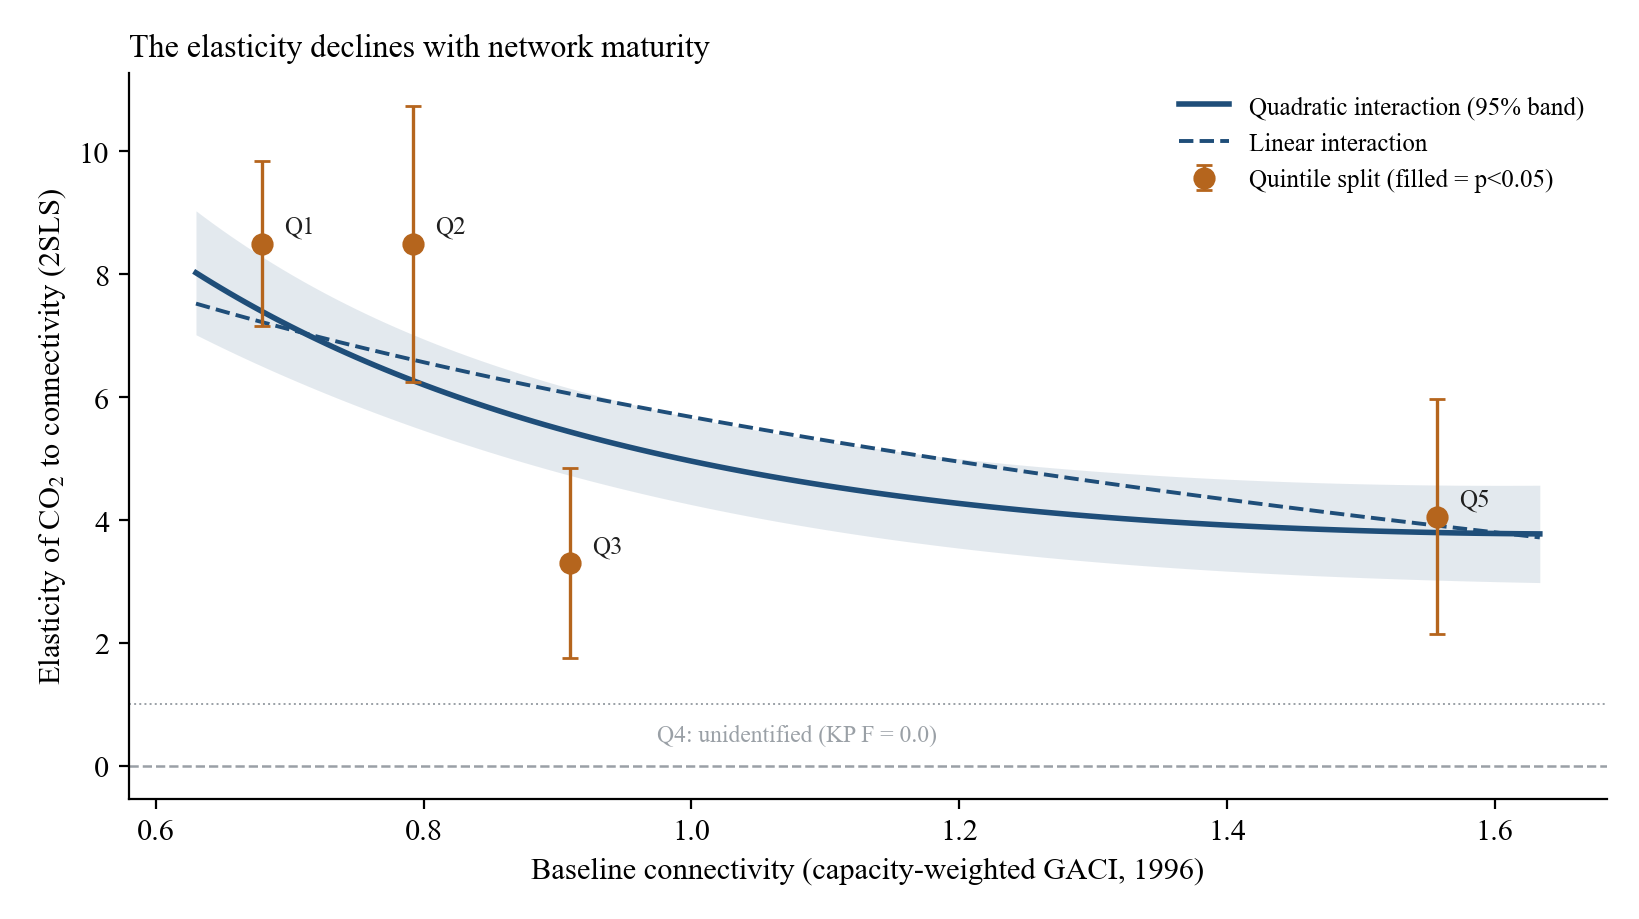
\includegraphics[width=0.85\textwidth]{CO2_gradient_baseline.png}
\caption{\textbf{The elasticity along the baseline-connectivity distribution.} Quintile split-sample 2SLS estimates (points, 95 percent confidence intervals; the fourth quintile is unidentified and omitted) and the fitted elasticity from pooled specifications that interact log GACI with centred log baseline GACI (linear, dashed; quadratic with 95 percent band). Horizontal lines mark zero and one.}
\label{fig:gradient}
\end{figure}

This reading matters for extrapolation. Applying a single elasticity to
every country, as the attribution in the next section does, overstates the
contribution of mature networks and understates that of new entrants.
Re-computing the attribution with tercile-specific elasticities, with the
fitted continuous elasticity at each country's baseline, or with the
semi-log slope applied to the absolute change in connectivity gives world
totals between 294 and 353 Mt, or 35 to 43 percent of 2023 emissions,
against 356 Mt under the common elasticity (Extended Data
Table~\ref{tab:attr_sens}). The headline attribution is therefore an upper
bound of a range whose lower end is about one third of current emissions.

\begin{figure}[htbp]
\centering
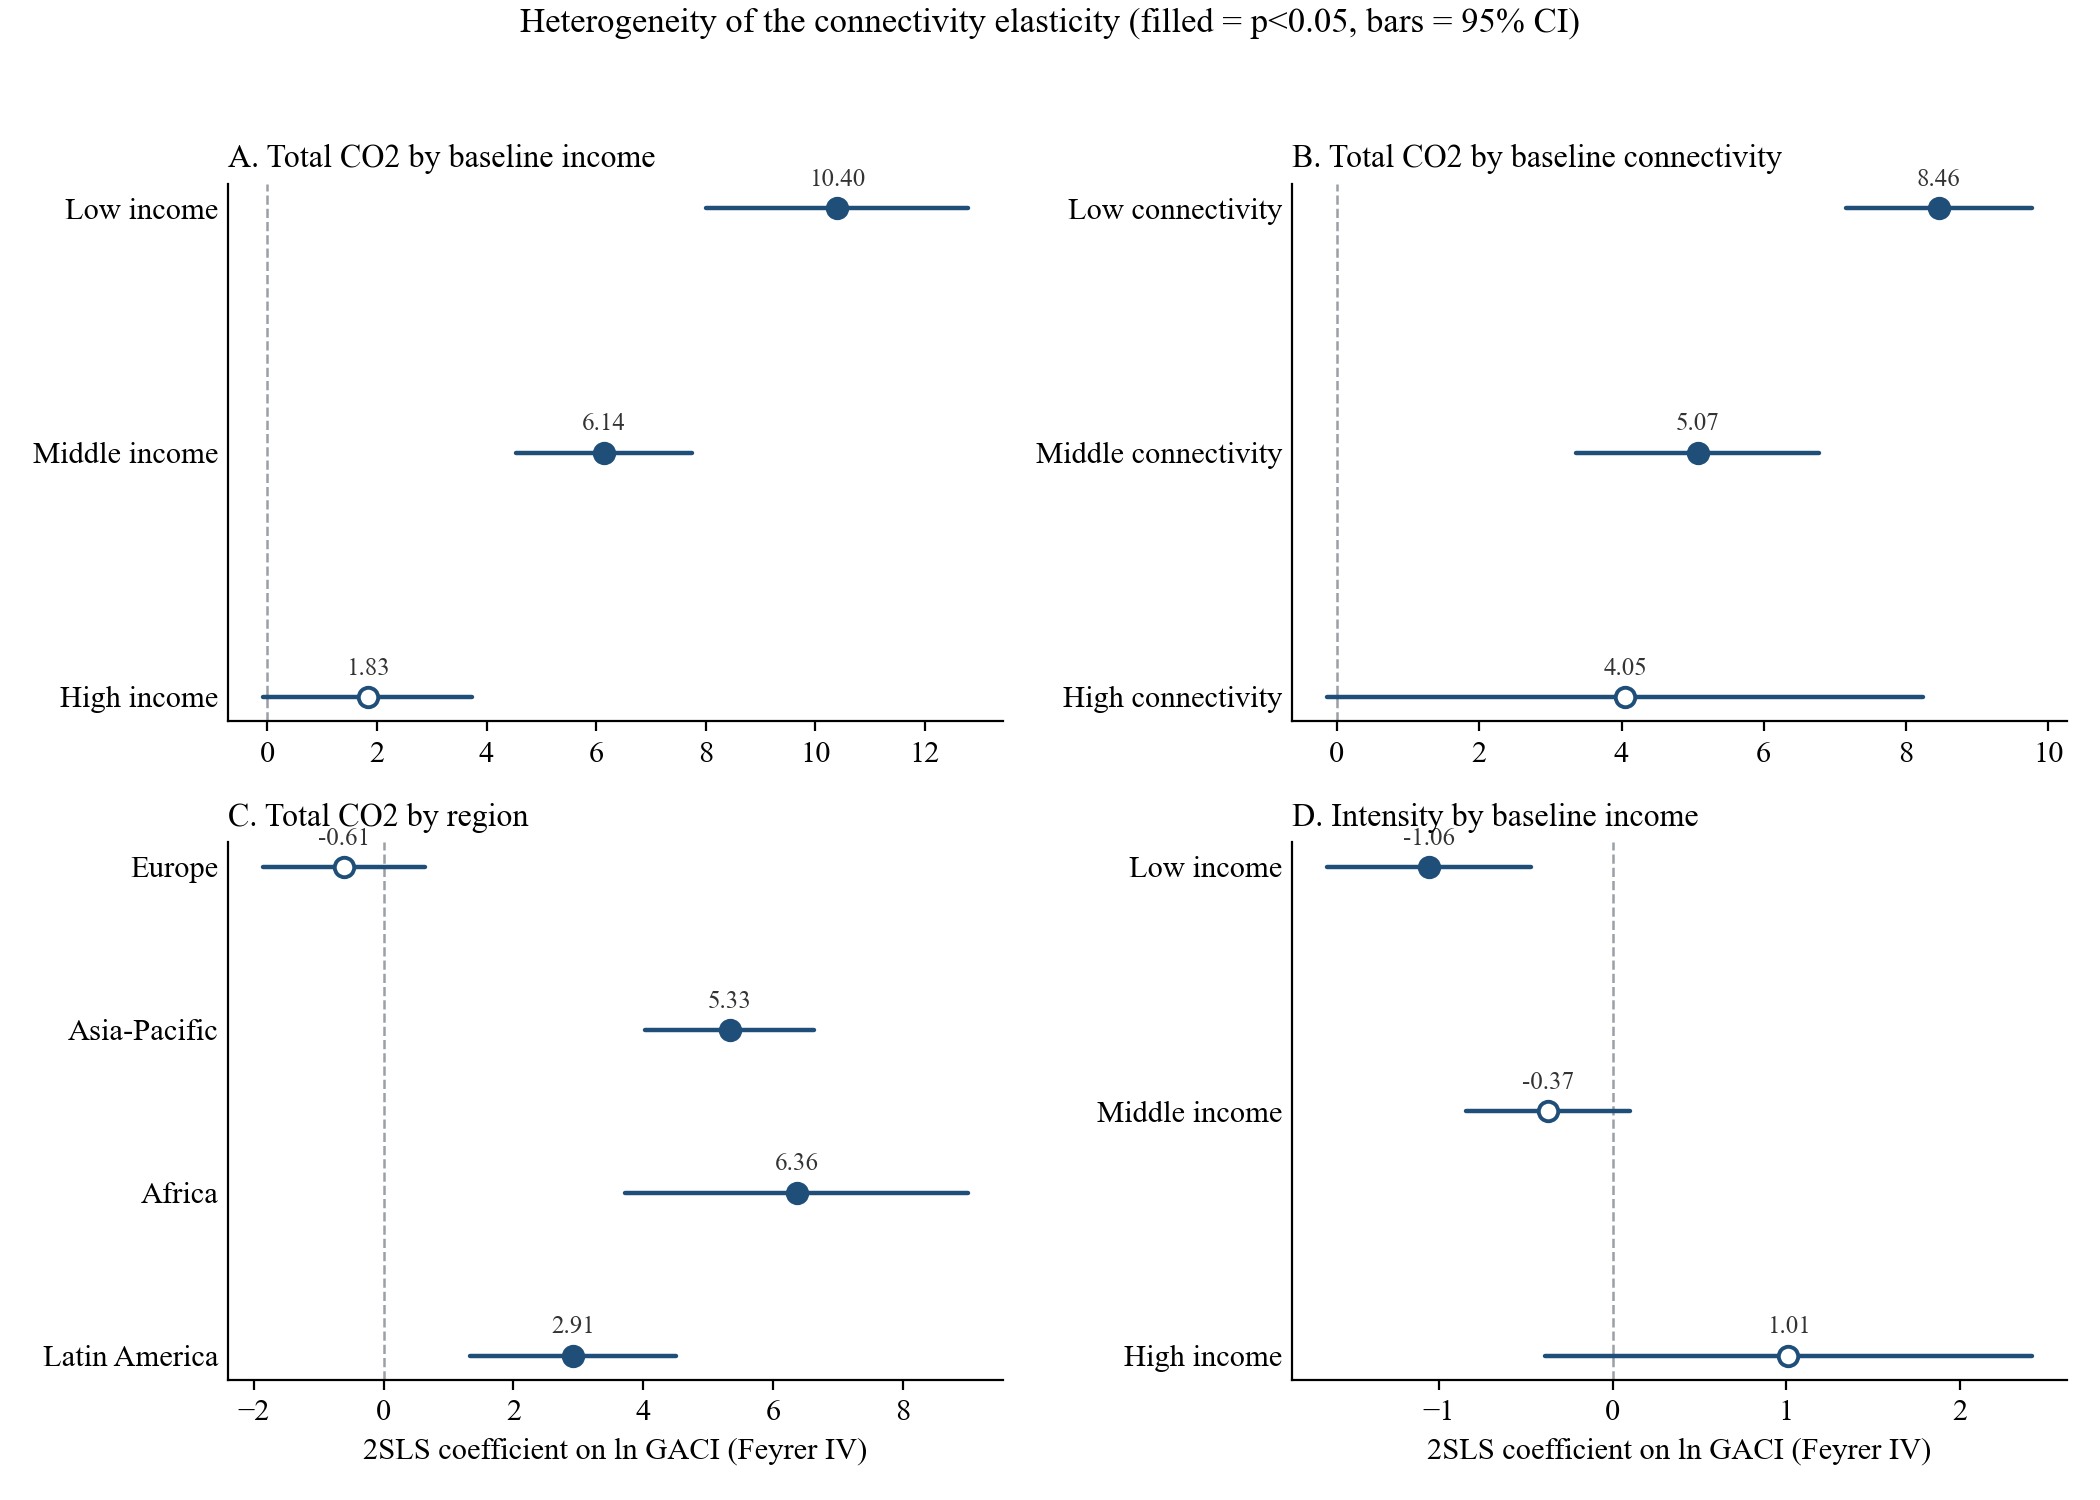
\includegraphics[width=0.92\textwidth]{CO2_hetero_coefplot.png}
\caption{\textbf{Heterogeneity of the connectivity elasticity} (2SLS, Feyrer instrument; total bunker CO$_2$ in panels A--C, CO$_2$ per seat-km in panel D). Filled markers denote $p<0.05$; bars are 95 percent confidence intervals. The Middle East and North America are omitted as unidentified.}
\label{fig:hetero}
\end{figure}

\subsection*{Emissions respond to contiguous neighbours' connectivity}
Emissions do not respond only to a country's own network. We define
neighbour connectivity as the leave-out average of other countries' log
GACI under a spatial weighting, instrument it with the identically weighted
average of their Feyrer shifters, and, unlike in a first version of this
analysis, instrument own connectivity at the same time (Methods).
Table~\ref{tab:spillover} reports the joint estimates. When neighbours are
the contiguous countries, a one percent increase in own connectivity raises
own bunker CO$_2$ by 3.48 percent and a one percent increase in the
neighbours' connectivity raises it by a further 1.93 percent (s.e.\ 0.27;
0.69 clustered by country), with conditional first-stage $F$ statistics of
66 and 124. Definitions that reach further give larger neighbour and
smaller own coefficients: 3.51 for the five nearest countries, 0.62 for
countries within 500 km, and 4.97 with a 1{,}000 km kernel, at which point
the own effect is no longer identified. The all-country inverse-distance
definition of the earlier draft cannot be jointly instrumented, because its
shifter is nearly collinear with the own shifter within country; with the
own shifter in reduced form it gives 7.45, but that estimate has a
country-clustered standard error of 5.7 and a permutation placebo, in which
countries are relabelled at random in the weight matrix, reproduces a
$t$-statistic as large as the actual one in 15 percent of draws (Extended
Data Table~\ref{tab:spill_ext} and Extended Data
Fig.~\ref{fig:spillplacebo}). The same placebo applied to the contiguity
and five-nearest specifications reproduces the actual $t$-statistic in 0.4
and 1.0 percent of draws. Because the joint specification has a weak
cluster-robust first stage (Kleibergen--Paap $F$ of 3.3 with standard
errors clustered by country; conditional $F$ of 6.7 and 13.2), we also
instrument neighbour connectivity alone with the own shifter as a control,
as in the earlier draft but with the contiguity definition: the neighbour
elasticity is 2.05 (s.e.\ 0.61 clustered by country; first-stage $F$ =
175), its Anderson--Rubin 95 percent set is 0.9 to 3.2, and it is 2.07
(s.e.\ 0.83) with sub-region-by-year fixed effects. The subset
Anderson--Rubin set for the neighbour coefficient in the joint
specification, 0.1 to 3.1, also excludes zero. The five-nearest and 500 km
definitions do not survive clustering (Anderson--Rubin sets that include
zero), so the spillover is a land-neighbour result, and we treat the
contiguity estimates as the spillover result.

The spatial profile explains why (Extended Data Fig.~\ref{fig:spilldecay}
and Extended Data Table~\ref{tab:spill_ext}). Taken one at a time, the
exposure to contiguous countries carries a coefficient of 2.05, the 0--500
km and 500--1{,}000 km bands carry nothing, the 1{,}000--2{,}000 km band
carries 2.51, and the band beyond 5{,}000 km carries a significantly
negative coefficient. A spillover that declined smoothly with distance
would not produce that pattern; exposures that average over most of the
world instead track global trends in the network, with signs that depend
on which countries dominate the average. The contiguity estimate survives
the addition of sub-region-by-year fixed effects, which absorb every
regional trend (1.95; s.e.\ 0.47 robust, 1.09 clustered by sub-region),
and it loads on international rather than domestic traffic (2.23 against
2.02 with a standard error of 0.90). Within aviation blocs the leave-out
exposure carries 2.35 (s.e.\ 0.32).

Panel B of Table~\ref{tab:spillover} places the own and neighbour margins
side by side under the contiguity definition. Own connectivity works
through frequency (5.61) with shorter stages and no up-gauging, as in
Table~\ref{tab:decomp}, although the own intensity coefficient in the
joint specification (0.32, s.e.\ 0.16 robust, 0.40 clustered) differs from
the single-equation estimate and should not be read as a reversal of the
efficiency margin; neighbours' connectivity raises own seat-kilometres by 2.56 percent
through more flights (1.22) on longer stages (1.04), leaves aircraft size
unchanged, raises the international share slightly, and lowers emissions
per seat-km by 0.63 percent. A neighbour's connectivity gain therefore
adds longer, more international and more efficient flying to the home
country, the signature of traffic feeding a regional hub, and national
estimates understate the network-wide emissions effect of connectivity
growth by a margin that, at the elasticities in Table~\ref{tab:spillover},
is of the order of half the own effect.

\begin{table}[htbp]
\centering
\begin{threeparttable}
\caption{Connectivity spillovers: own and neighbouring countries' connectivity, jointly instrumented}
\label{tab:spillover}
\footnotesize
\begin{tabular}{lccccc}
\toprule
\multicolumn{6}{l}{\textit{Panel A. Log bunker CO$_2$; own and neighbour connectivity both instrumented}} \\
Neighbour definition & Own ln GACI & Neighbour ln GACI & SW $F$ (own / nbr) & KP $F$ & $N$ \\
\midrule
  Contiguous countries (land border) & 3.48$^{***}$ (0.47) & 1.93$^{***}$ (0.27) & 66 / 124 & 32.7 & 4,623 \\
  \quad s.e.\ clustered by country & (1.29) & (0.69) & & & \\
  Five nearest countries & 1.23$^{*}$ (0.64) & 3.51$^{***}$ (0.66) & 48 / 49 & 23.5 & 4,623 \\
  \quad s.e.\ clustered by country & (1.84) & (1.94) & & & \\
  Countries within 500 km & 4.89$^{***}$ (0.52) & 0.62$^{**}$ (0.26) & 104 / 224 & 51.2 & 4,623 \\
  \quad s.e.\ clustered by country & (1.34) & (0.66) & & & \\
  Kernel $\exp(-d/1000\,\mathrm{km})$ & -0.08 (0.66) & 4.97$^{***}$ (0.77) & 41 / 49 & 20.5 & 4,623 \\
  \quad s.e.\ clustered by country & (1.91) & (2.29) & & & \\
  Inverse distance, all countries & -2.35 (1.69) & 16.18$^{***}$ (3.74) & 10 / 11 & 5.1 & 4,623 \\
\midrule
\multicolumn{6}{l}{\textit{Neighbour connectivity instrumented, own shifter in reduced form; s.e.\ clustered by country; AR = Anderson--Rubin 95\% set}} \\
Neighbour definition & Own shifter (RF) & Neighbour ln GACI & AR set & KP $F$ & $N$ \\
  Contiguous countries & controlled & 2.05$^{***}$ (0.61) & [0.9, 3.2] & 175.2 & 4,623 \\
  Contiguous, sub-region $\times$ year FE & controlled & 2.07$^{**}$ (0.83) & -- & 97.5 & 4,621 \\
  Countries within 500 km & controlled & 0.09 (0.90) & [-1.7, 1.8] & 88.3 & 4,623 \\
  Five nearest countries & controlled & 7.05 (5.59) & [-0.1, 12.0] & 1.5 & 4,623 \\
  Contiguous, joint 2SLS (own and neighbour instrumented) & own 3.48$^{***}$ (1.29) & 1.93$^{***}$ (0.69) & [0.1, 3.1] & 3.3 (SW 6.7 / 13.2) & 4,623 \\
  Within 500 km, joint 2SLS & own 4.84$^{***}$ (1.33) & 0.67 (0.65) & [-0.7, 1.9] & 6.6 (SW 13.3 / 31.3) & 4,623 \\
  Inverse distance, own shifter in reduced form (previous specification) & RF 0.25$^{**}$ (0.12) & 7.45$^{***}$ (1.99) & -- & 134.1 & 4,623 \\
  \quad s.e.\ clustered by country & & (5.66) & & & \\
\midrule
\multicolumn{6}{l}{\textit{Panel B. Margins of the response, contiguity definition, joint 2SLS}} \\
Outcome & Own ln GACI & Neighbour ln GACI & & KP $F$ & $N$ \\
\midrule
  Bunker CO$_2$ & 3.48$^{***}$ (0.47) [1.29] & 1.93$^{***}$ (0.27) [0.69] & & 32.7 & 4,623 \\
  International CO$_2$ & 3.15$^{***}$ (0.46) [1.24] & 2.23$^{***}$ (0.26) [0.63] & & 32.5 & 4,622 \\
  Domestic CO$_2$ & -2.72 (1.77) [4.63] & 2.02$^{**}$ (0.90) [2.34] & & 26.2 & 3,567 \\
  Seat-km & 3.16$^{***}$ (0.49) [1.39] & 2.56$^{***}$ (0.27) [0.69] & & 32.7 & 4,623 \\
  Flights & 5.61$^{***}$ (0.79) [2.10] & 1.22$^{**}$ (0.54) [1.41] & & 32.7 & 4,623 \\
  Seats per flight & -0.65$^{*}$ (0.34) [0.84] & 0.30 (0.25) [0.61] & & 32.7 & 4,623 \\
  Km per flight & -1.80$^{***}$ (0.40) [1.21] & 1.04$^{***}$ (0.25) [0.71] & & 32.7 & 4,623 \\
  CO$_2$ per seat-km & 0.32$^{**}$ (0.16) [0.40] & -0.63$^{***}$ (0.10) [0.23] & & 32.7 & 4,623 \\
  International share of seat-km & 0.01 (0.07) [0.17] & 0.07$^{*}$ (0.04) [0.09] & & 32.7 & 4,623 \\
\bottomrule
\end{tabular}
\begin{tablenotes}[flushleft]
\footnotesize
\item Notes: Neighbour connectivity is the leave-out average of other countries' log GACI (capacity-weighted mean) under the stated weighting; it is instrumented by the identically weighted average of their Feyrer shifters, and own connectivity by the own shifter. All specifications include country and year fixed effects, log population, log sea market access and an indicator for countries with no neighbour under the definition (31 countries have no land neighbour). SW $F$ is the Sanderson--Windmeijer conditional first-stage statistic for each endogenous regressor. Heteroskedasticity-robust standard errors in parentheses; country-clustered standard errors in brackets or on the following line. The middle block of Panel A instruments neighbour connectivity only, with the own shifter as a control, and reports country-clustered standard errors and Anderson--Rubin 95 percent sets obtained by grid inversion (for the joint rows, the subset Anderson--Rubin set for the neighbour coefficient with own connectivity instrumented under each null); SW $F$ in that block is cluster-robust. The last row is the specification of the previous draft with all-country inverse-distance weights. $^{***}$, $^{**}$, $^{*}$: significance at 1, 5, and 10 percent (robust).
\end{tablenotes}
\end{threeparttable}
\end{table}

\subsection*{Connectivity growth accounts for 42.5 percent of 2023
emissions}
Applying the estimated elasticity to each country's connectivity change
since 1996 attributes 356 Mt, or 42.5 percent, of 2023 aviation CO$_2$ to
post-1996 network expansion (Fig.~\ref{fig:attributed}; Methods). The
attributed growth is concentrated in emerging hub countries: China
($+88$ Mt), the United States ($+36$), the United Arab Emirates ($+25$),
Japan ($+17$), Turkey ($+17$), India ($+16$), and Korea ($+14$), while
Germany's declining connectivity contributes $-16$ Mt (Table~\ref{tab:scc} and Fig.~\ref{fig:bars}); with elasticities that vary by baseline connectivity the world total is 294 to 353 Mt (Extended Data Table~\ref{tab:attr_sens}). Valued at standard social-cost-of-carbon estimates,
these emissions represent an annual external cost of \$18.2 billion to
\$67.7 billion, depending on whether the US Interagency Working Group
interim value (\$51 per tonne), the Rennert et al.\ estimate (\$185), or
the US EPA central value (\$190) is applied [TODO cite]; at the EPA value
the cost is \$16.7 billion per year for China, \$6.9 billion for the
United States, and \$4.7 billion for the United Arab Emirates, while
Germany's connectivity decline corresponds to an avoided cost of \$3.0
billion per year. Where these
emissions are generated is, moreover, not where they are booked: the
bunker-attributed share of world emissions exceeds the physical
landing-and-take-off share by 1.4 percentage points for the United States
and the United Arab Emirates, while China's attributed share falls short by
3.5 points, a gap that is positive at every international mega-hub and
negative at large domestically oriented hubs (Figs.~\ref{fig:levels} and \ref{fig:mismatch}). Any scheme that allocates
responsibility by booked emissions, including CORSIA, embeds a transfer
across these accounting boundaries. The airport concentration results add
a practical corollary: an instrument that covered the top five percent of
airports by attributed emissions, some 190 nodes, would cover 85 percent
of the connectivity-driven total, and one covering the top ten percent
would cover 94 percent.

\begin{figure}[htbp]
\centering
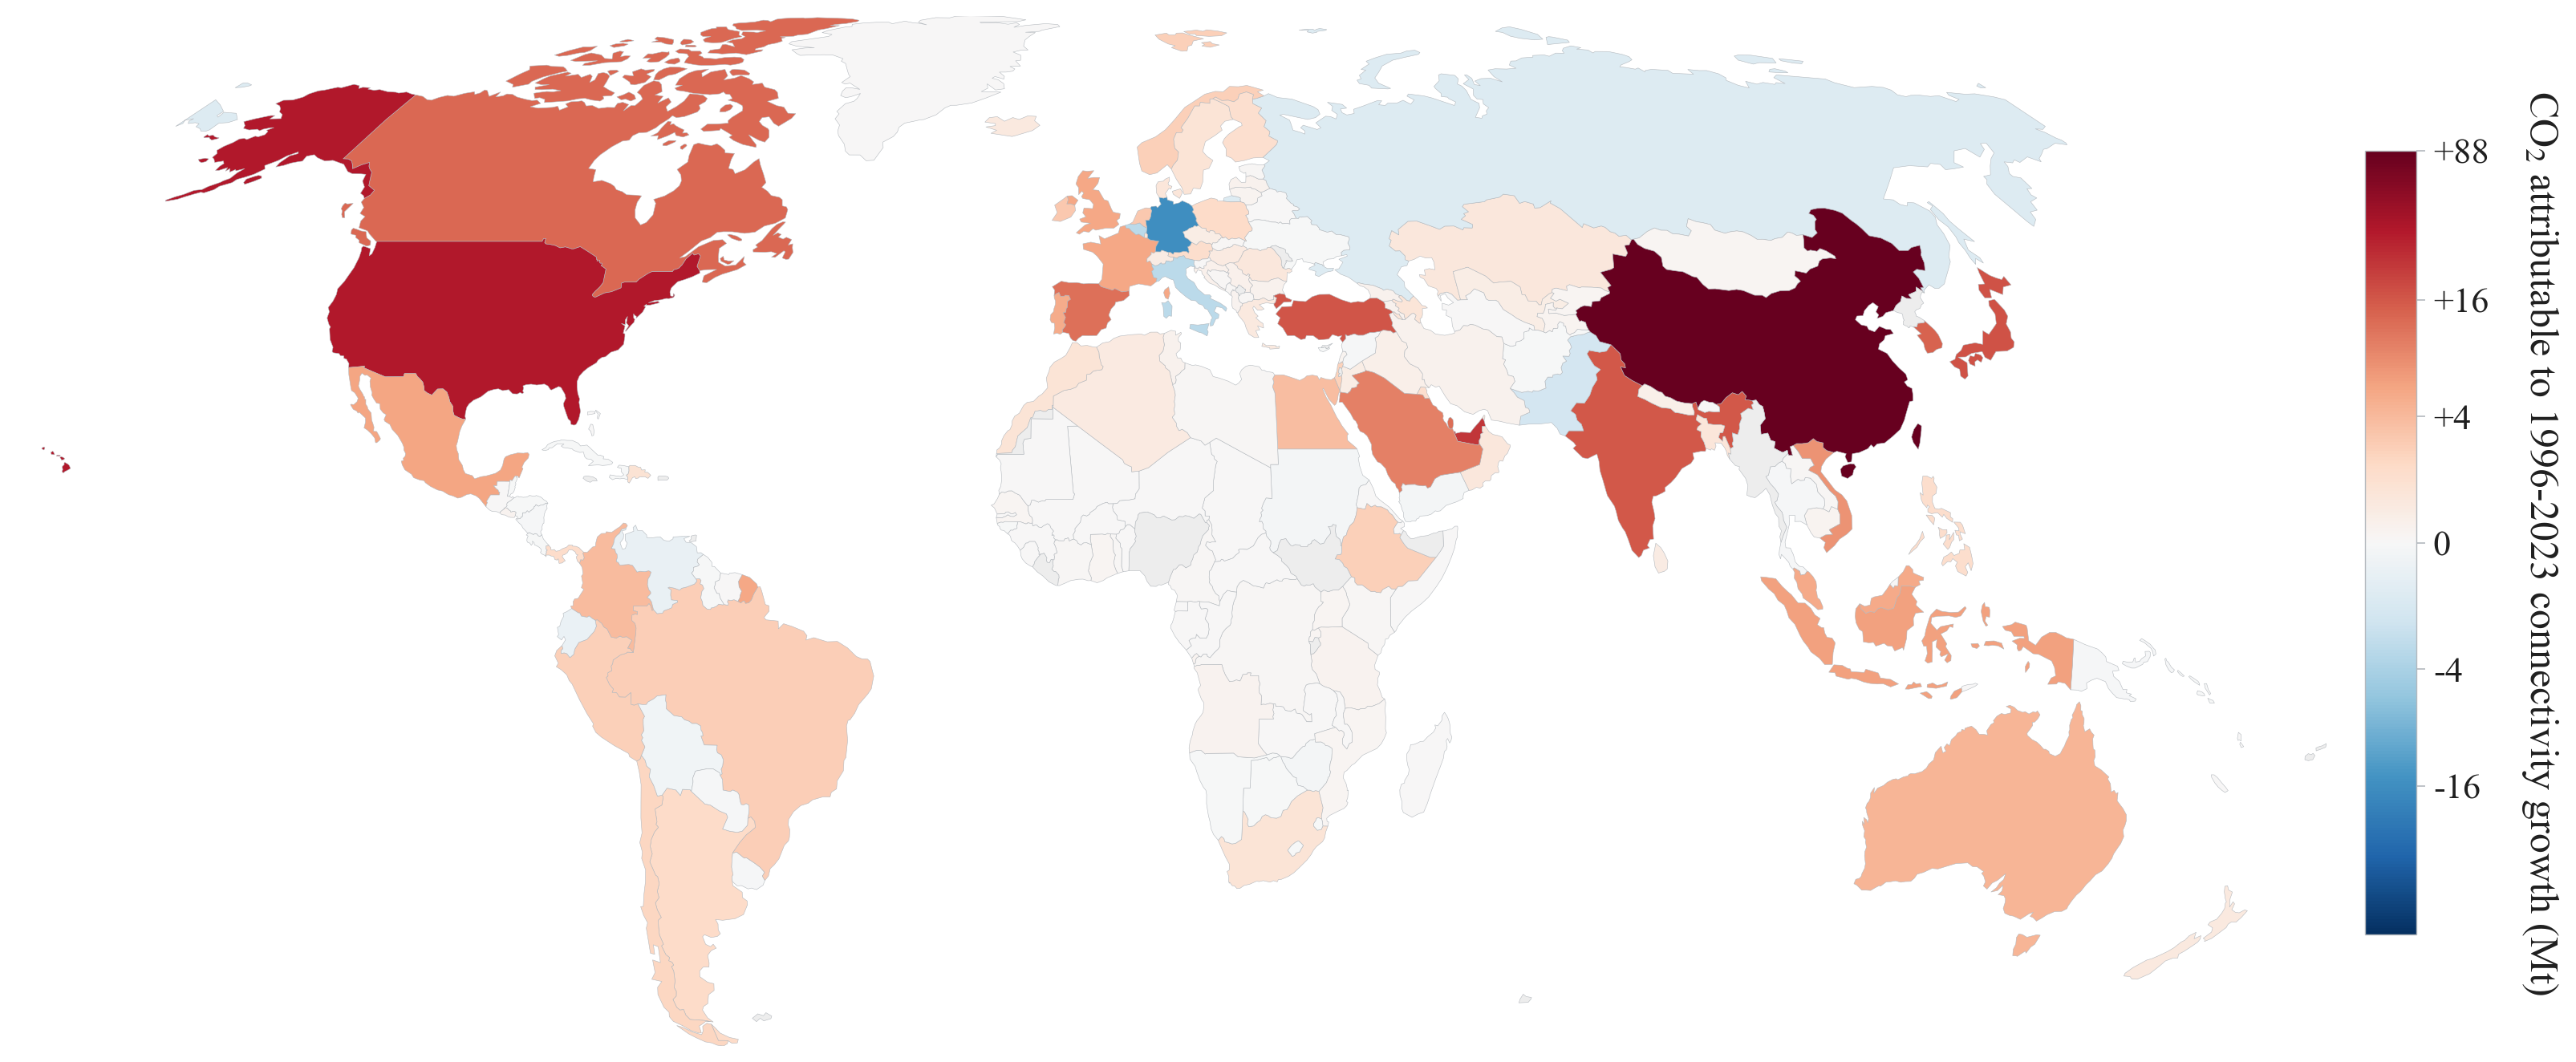
\includegraphics[width=0.92\textwidth]{CO2_map_attributed_2023.png}
\caption{\textbf{Aviation CO$_2$ attributed to post-1996 connectivity growth, 2023 (Mt).} White denotes zero; the attribution applies the Feyrer-instrument elasticity to each country's connectivity change.}
\label{fig:attributed}
\end{figure}

\begin{table}[htbp]
\centering
\begin{threeparttable}
\caption{Country-level attribution and social cost of connectivity-driven aviation CO$_2$, 2023}
\label{tab:scc}
\footnotesize
\begin{tabular}{lcccccc}
\toprule
 & & \multicolumn{2}{c}{Attributed CO$_2$ (Mt)} & \multicolumn{3}{c}{Social cost (\$bn per year)} \\
\cmidrule(lr){3-4}\cmidrule(lr){5-7}
 & $\Delta \ln$ GACI & Total & International & SCC \$51 & SCC \$185 & SCC \$190 \\
\midrule
China          & 0.33  & 87.7  & 16.9  & 4.5  & 16.2 & 16.7 \\
United States  & 0.04  & 36.4  & 13.6  & 1.9  & 6.7  & 6.9  \\
United Arab Emirates & 0.57 & 24.7 & 24.7 & 1.3 & 4.6 & 4.7 \\
Japan          & 0.19  & 17.4  & 10.4  & 0.9  & 3.2  & 3.3  \\
Turkey         & 0.55  & 16.6  & 13.5  & 0.8  & 3.1  & 3.2  \\
India          & 0.19  & 15.9  & 7.6   & 0.8  & 2.9  & 3.0  \\
Korea          & 0.71  & 14.1  & 12.8  & 0.7  & 2.6  & 2.7  \\
Canada         & 0.22  & 13.1  & 8.5   & 0.7  & 2.4  & 2.5  \\
Qatar          & 0.80  & 12.2  & 12.2  & 0.6  & 2.3  & 2.3  \\
Spain          & 0.14  & 11.8  & 9.5   & 0.6  & 2.2  & 2.3  \\
Germany        & $-0.09$ & $-15.8$ & $-15.2$ & $-0.8$ & $-2.9$ & $-3.0$ \\
\midrule
World          &       & 356.4 & 212.0 & 18.2 & 65.9 & 67.7 \\
\bottomrule
\end{tabular}
\begin{tablenotes}[flushleft]
\footnotesize
\item Notes: Attributed CO$_2$ applies the Feyrer-instrument elasticities (5.669 total, 5.690 international) to each country's 1996--2023 change in log connectivity: attributed share $= 1-\exp(-\beta\,\Delta\ln\mathrm{GACI}_c)$, applied to 2023 emission levels under the bunker convention. Social cost values one year's attributable emissions at three social-cost-of-carbon estimates (2020 USD per tonne of CO$_2$): the US Interagency Working Group interim value (\$51, 3 percent discount rate), Rennert et al.\ (2022) (\$185, 2 percent near-term discount rate), and the US EPA (2023) central value (\$190, 2 percent Ramsey discounting); the valuation recurs annually while the traffic persists. Top ten positive countries, Germany (largest negative), and the world total (184 countries); the world attributed total equals 42.5 percent of 2023 aviation CO$_2$. Because the elasticity exceeds one, country-level attributed shares are extreme for fast growers; the figures are partial-equilibrium accounting.
\end{tablenotes}
\end{threeparttable}
\end{table}

\begin{figure}[htbp]
\centering
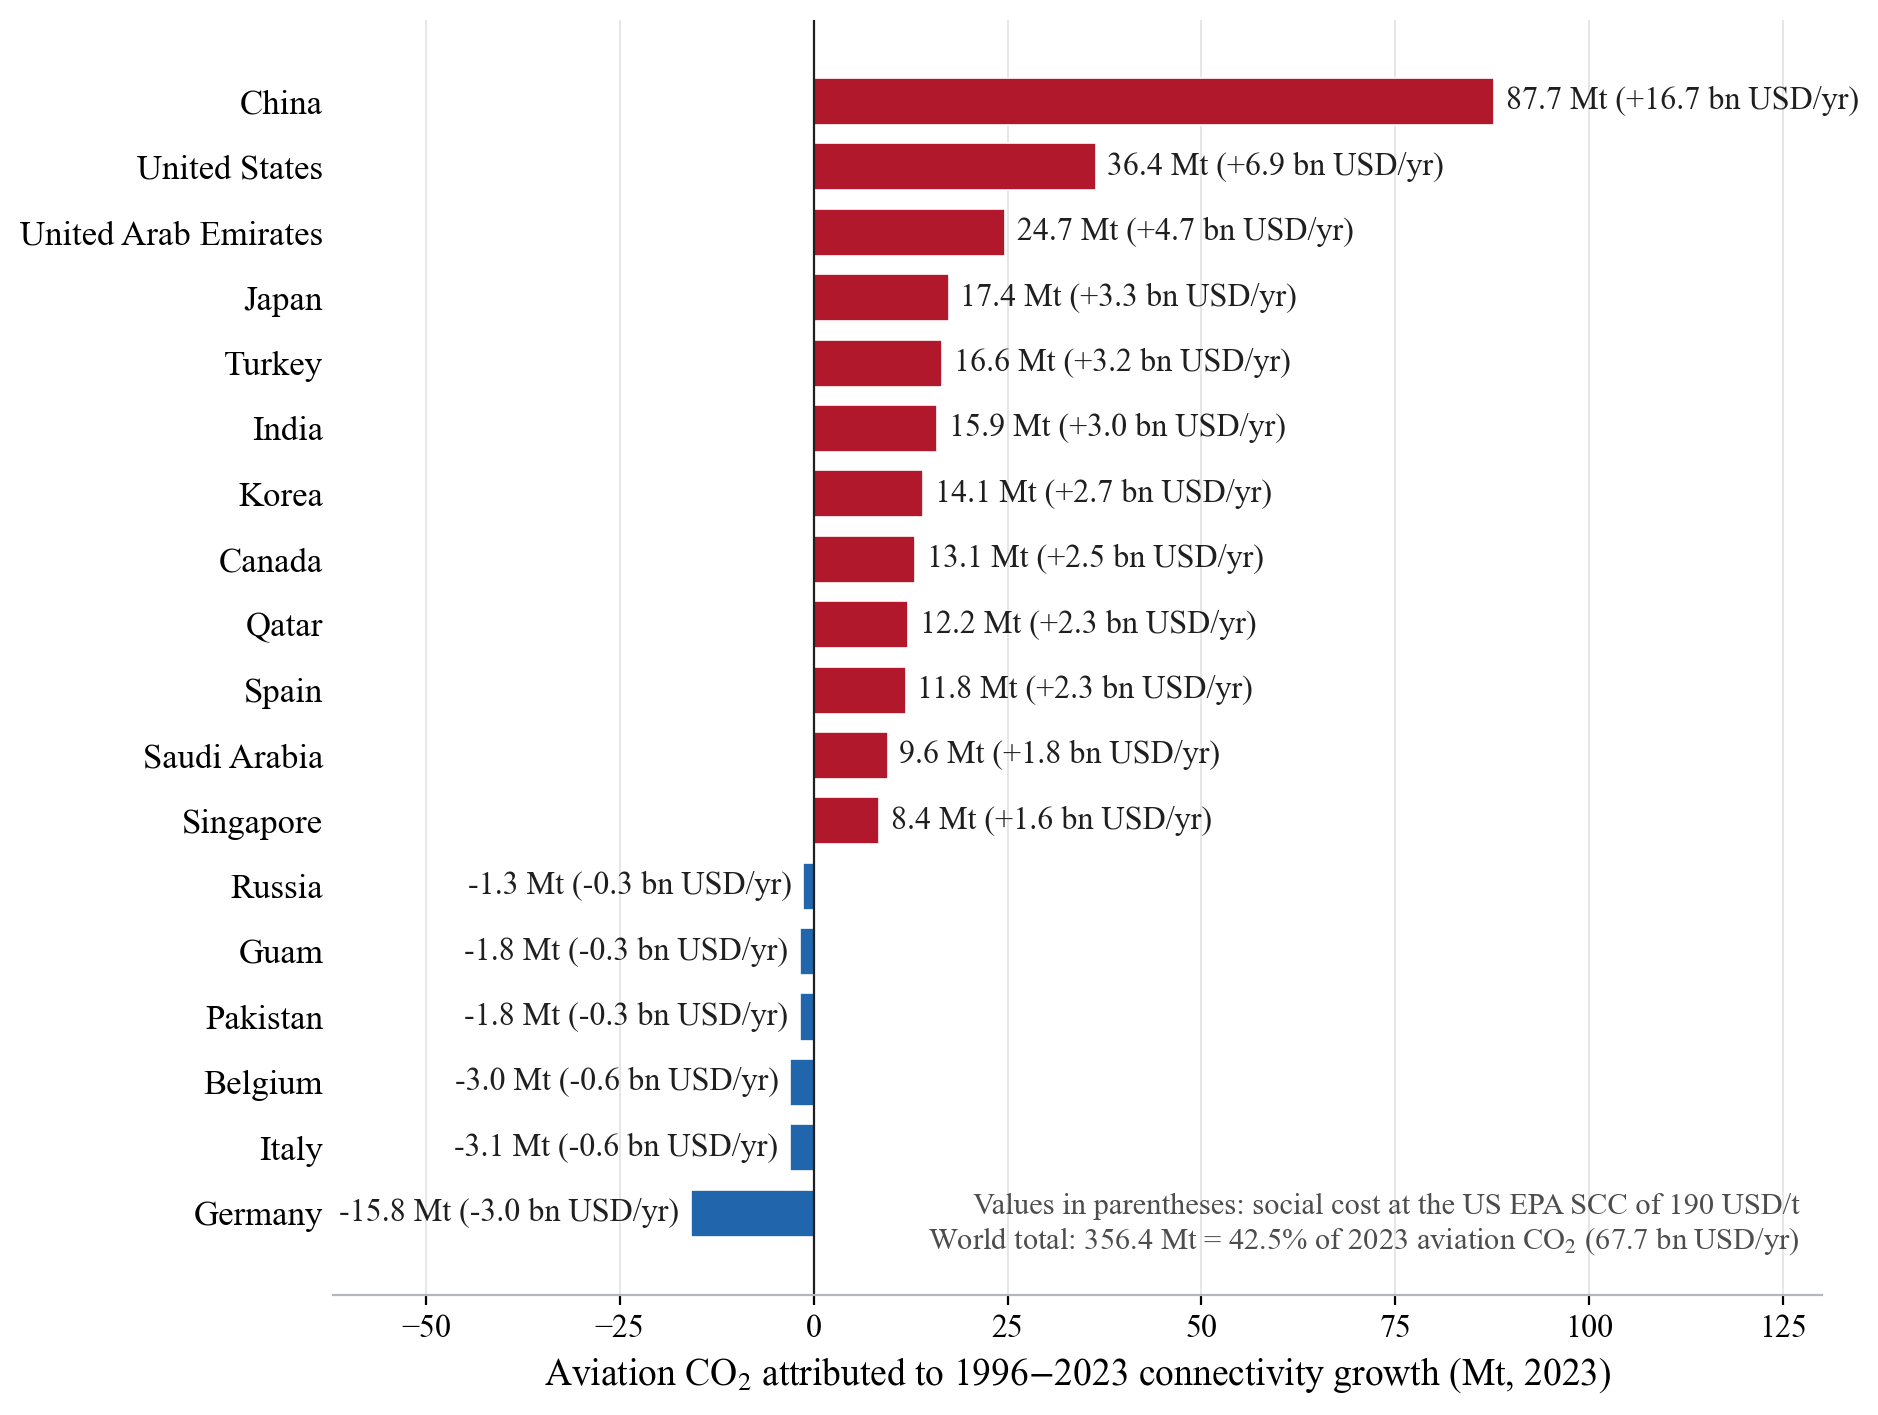
\includegraphics[width=0.92\textwidth]{CO2_attribution_bars.png}
\caption{\textbf{Country-level aviation CO$_2$ attributed to 1996--2023
connectivity growth, with its social cost.} Top twelve positive countries
and all countries below $-1$ Mt; parenthetical values apply the US EPA
social cost of carbon (\$190 per tonne). The world total is 356.4 Mt, 42.5
percent of 2023 aviation CO$_2$ (\$67.7 billion per year).}
\label{fig:bars}
\end{figure}

\begin{figure}[htbp]
\centering
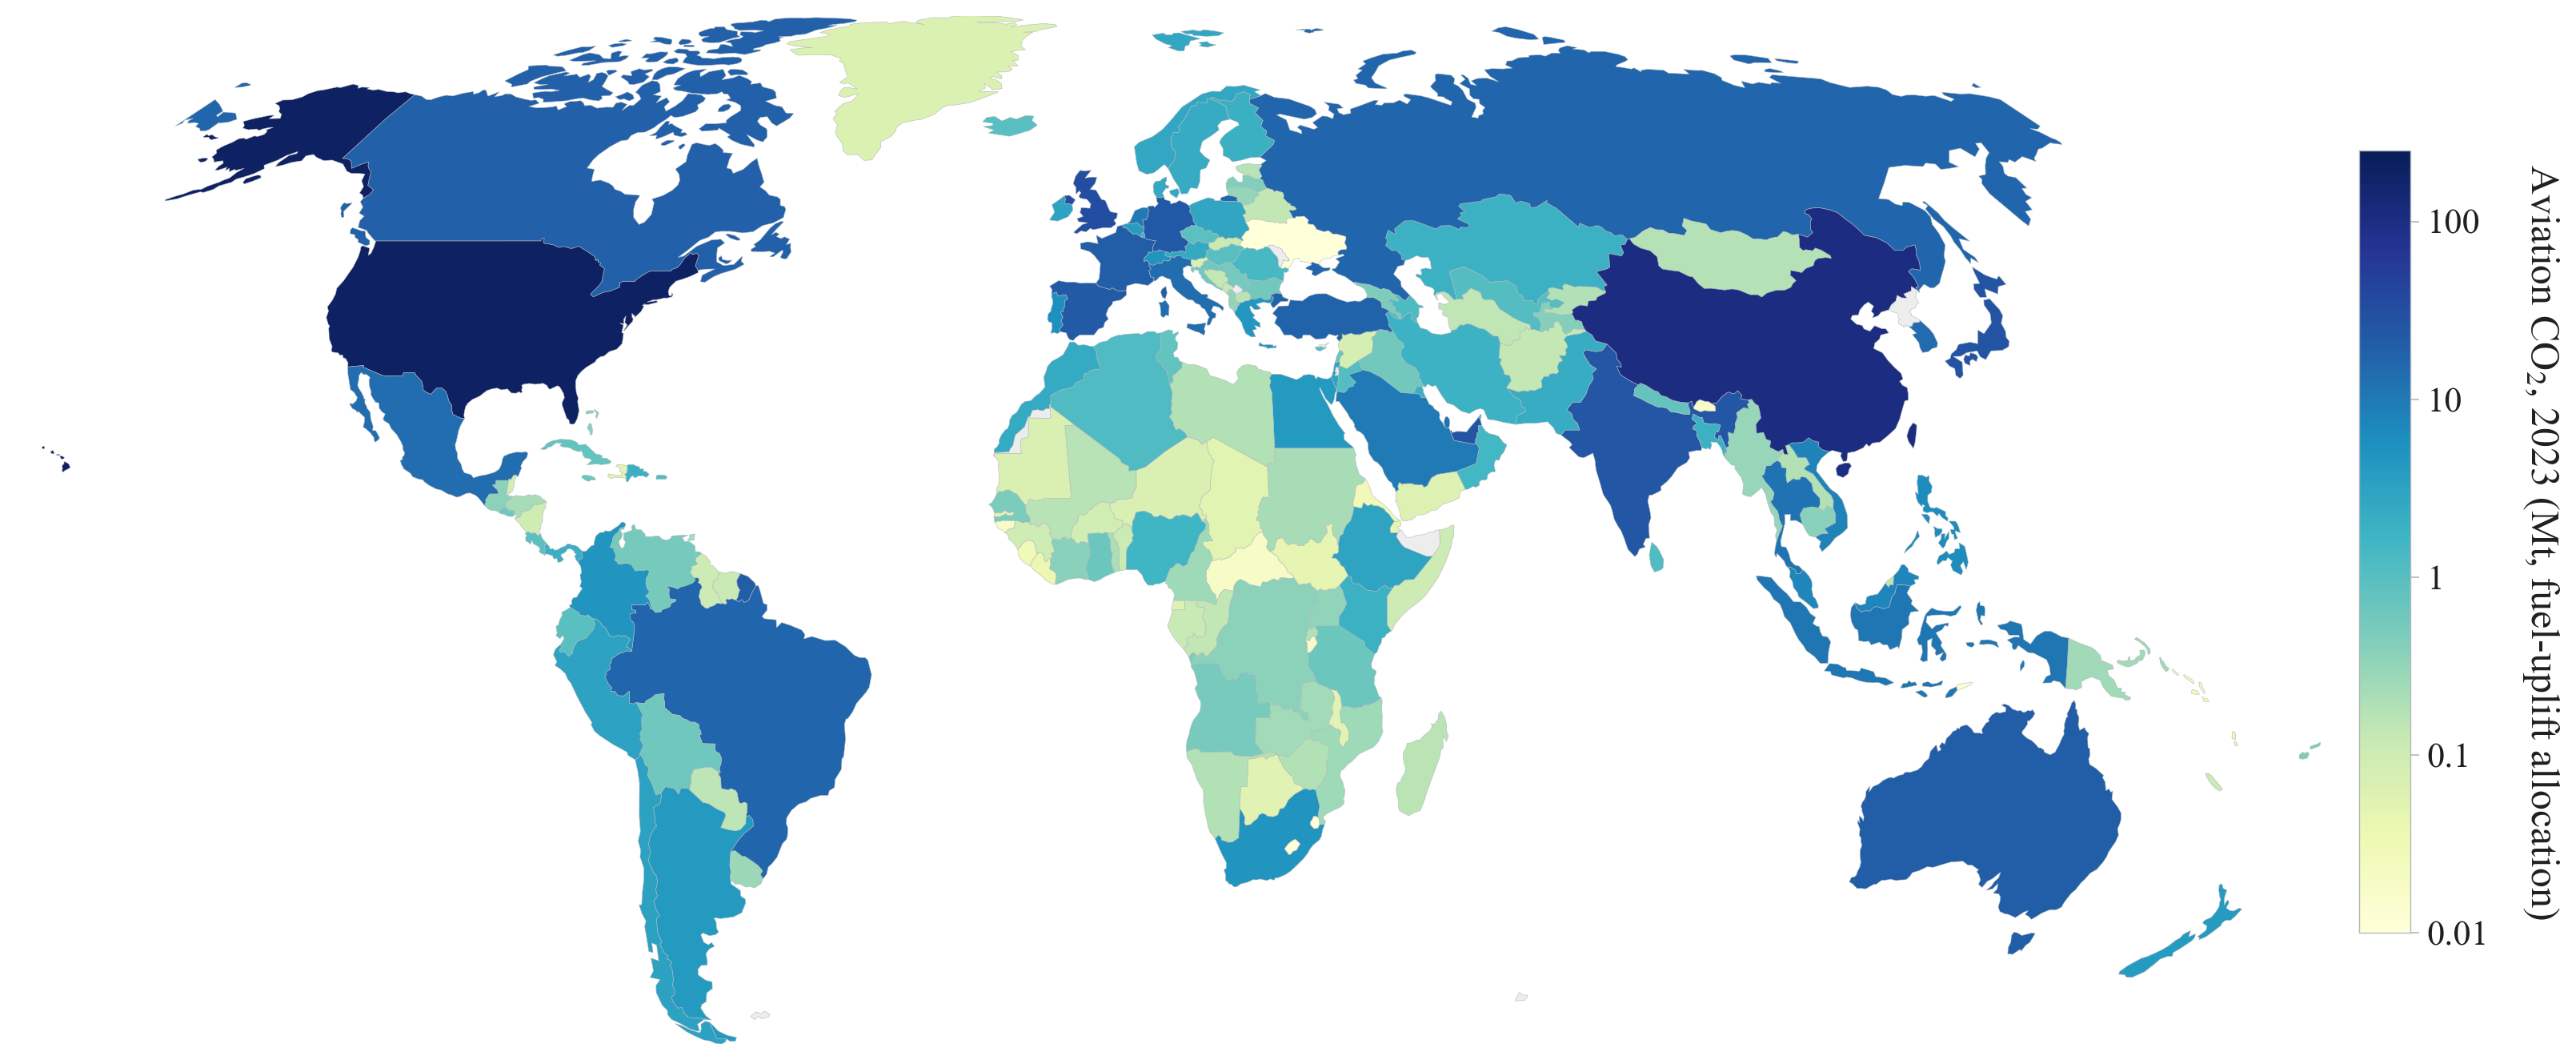
\includegraphics[width=0.92\textwidth]{CO2_map_levels_2023.png}
\caption{\textbf{Aviation CO$_2$ levels under the bunker convention, 2023.}}
\label{fig:levels}
\end{figure}

\begin{figure}[htbp]
\centering
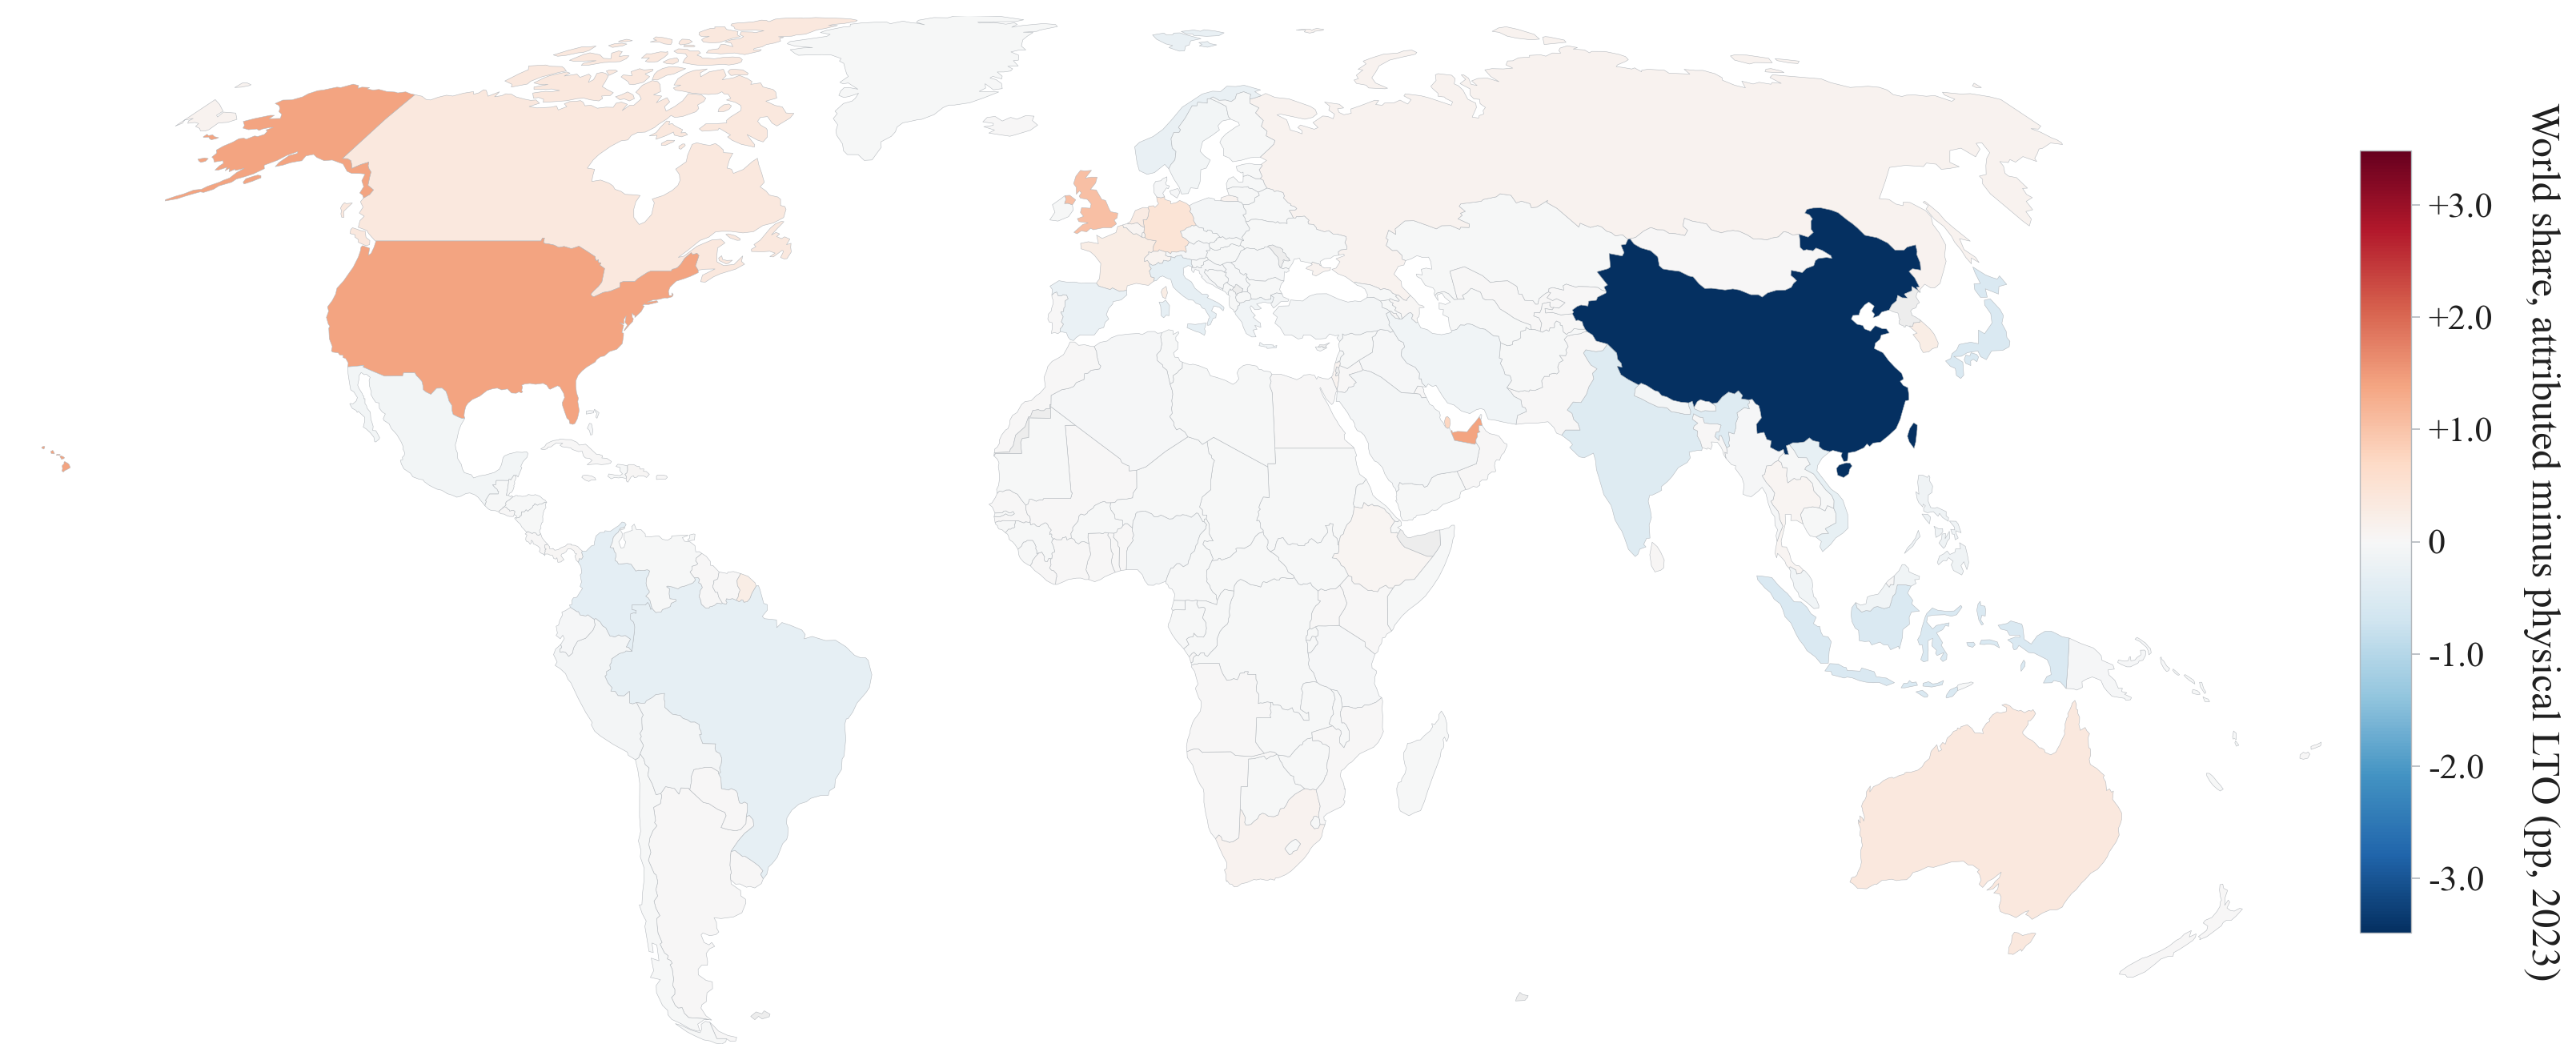
\includegraphics[width=0.92\textwidth]{CO2_map_mismatch_2023.png}
\caption{\textbf{Attribution mismatch, 2023:} bunker-attributed share minus physical LTO share (percentage points). Positive values indicate international hub countries; negative values indicate domestically oriented networks.}
\label{fig:mismatch}
\end{figure}

\subsection*{Only fuel switching materially lowers the level}
Since the efficiency margin offsets seven percent of the scale margin, the
level of emissions can be materially lowered only by changing the fuel
burned. Backing fuel quantities out of the 2023 total of 838 Mt and
applying ReFuelEU-style blending paths, the 2035 mandate lowers the total
to 704--754 Mt and the 2050 mandate to 369--545 Mt, depending on the
life-cycle saving of sustainable aviation fuel (Fig.~\ref{fig:saf};
Methods). The full 2050 blending path with a life-cycle saving of at least
65 percent would offset emissions of the same magnitude as those attributed
to the connectivity growth of the past generation.

\begin{figure}[htbp]
\centering
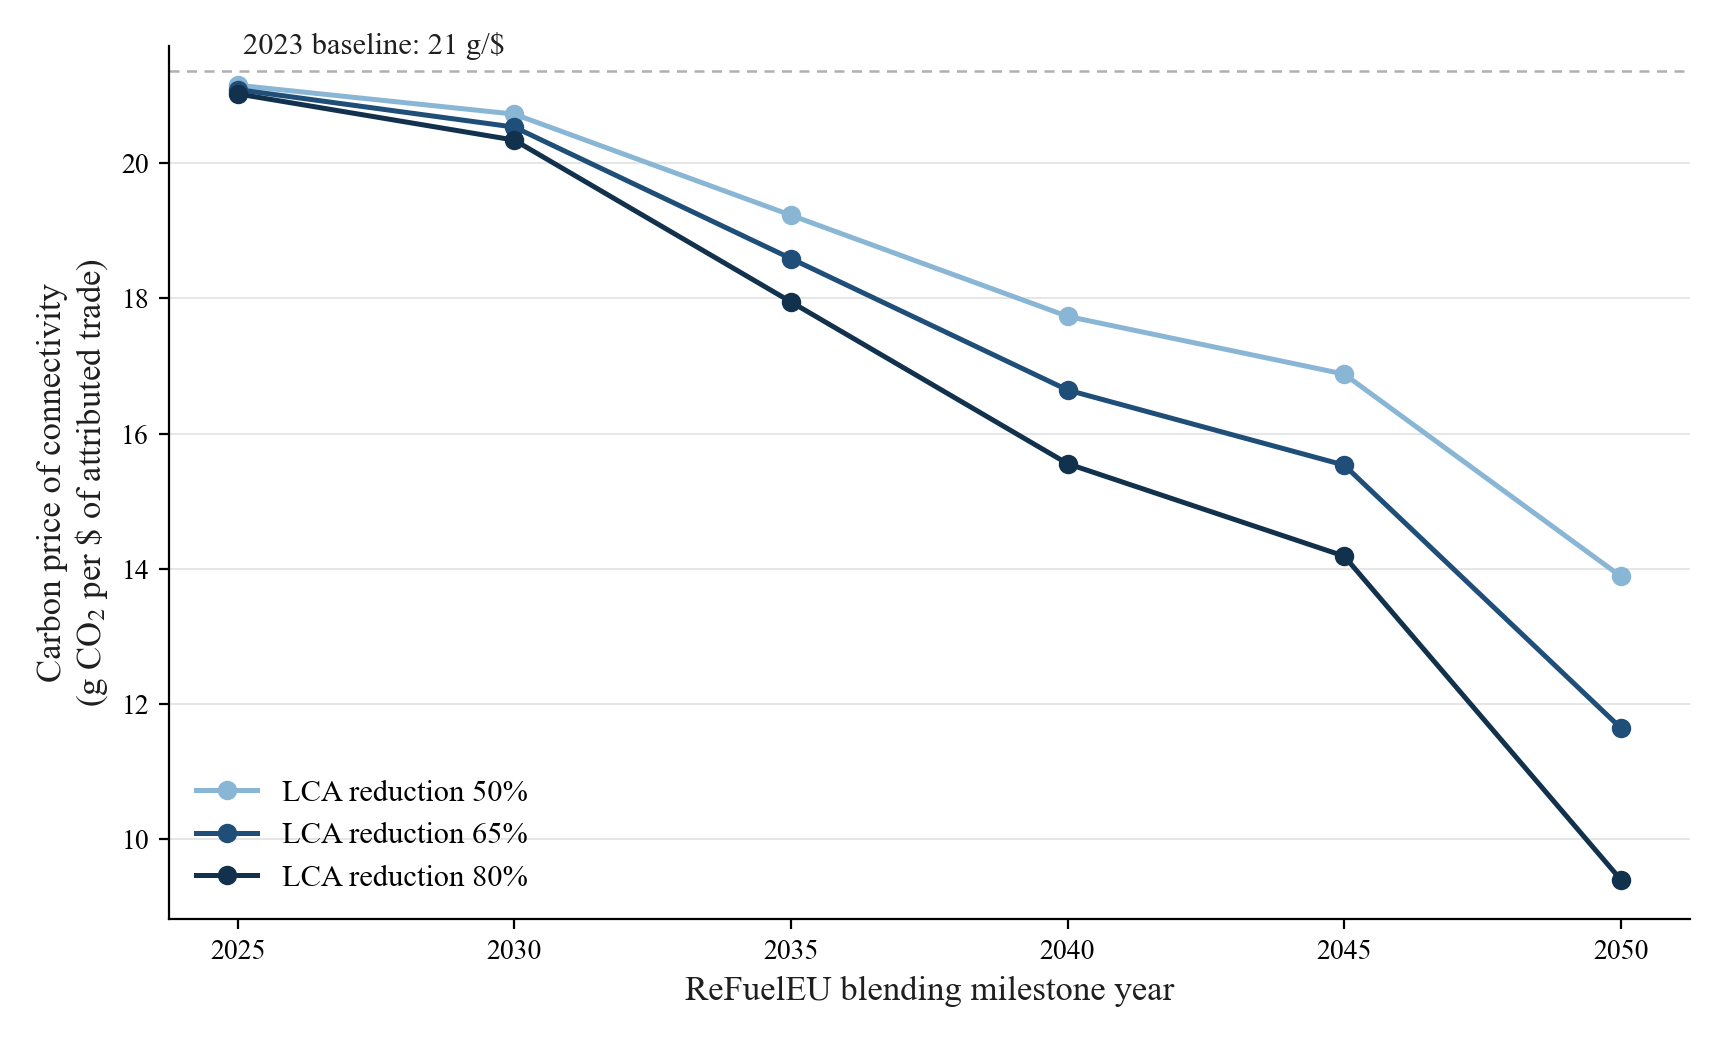
\includegraphics[width=0.92\textwidth]{CO2_saf_scenarios.png}
\caption{\textbf{World aviation CO$_2$ under ReFuelEU-style SAF blending paths.}}
\label{fig:saf}
\end{figure}

\subsection*{Attribution and fuel-switching scenarios [Ray and Lisa]}
The share of 2023 emissions attributed to post-1996 connectivity growth is
$1 - \exp(-\beta\,\Delta \ln \mathrm{GACI}_c)$, applied to 2023 levels;
because $\beta$ far exceeds one, country-level shares are extreme for
fast-growing countries and the world total (42.5 percent) is the more
conservative summary. The airport-level attribution applies the same
formula to each airport's change in log GACI between 1996, or its first
year in the network, and 2023; its sum (345 Mt) is close to the country
total because the elasticity is applied to the same emissions base. Fuel-switching scenarios back fuel out of emissions
at 3.15 kg CO$_2$ per kg and apply ReFuelEU-style blending shares (2 to 70
percent over 2025--2050) with life-cycle savings of 50, 65, and 80 percent,
holding 2023 traffic fixed; the calculations are partial-equilibrium
accounting. Attributed emissions are monetised at three
social-cost-of-carbon estimates, in 2020 USD per tonne of CO$_2$: the US
Interagency Working Group interim value (\$51, 3 percent discount rate),
the estimate of Rennert et al.\ (2022) (\$185, 2 percent near-term
discount rate), and the US EPA (2023) central value (\$190, 2 percent
Ramsey discounting) [TODO cite]. The valuation applies to one year's
attributable emissions and recurs annually while the connectivity-driven
traffic persists.

%=======================================================================
\section*{Discussion [Jinwoo]}
%=======================================================================
Three implications follow. First, for climate policy, the efficiency gains
that accompany network development are not a decarbonisation strategy. The
decomposition shows that connectivity growth is a frequency response, that
aircraft do not become larger, and that the technique margin offsets seven
percent of the scale response at the country level; the margin is present
at the airport level as well, but only sustained fuel switching materially
lowers the emissions level. Policies that promote connectivity on economic
grounds should be evaluated jointly with fuel and demand-side instruments
rather than on the expectation that hub efficiency will absorb the growth
in traffic.

Second, for the geography of mitigation burden, the results identify three
distinct wedges. The airport results show that the response is systemic
but that its emissions accumulate at the new hubs, so that a small number
of nodes would give an instrument most of its coverage. The spillover
estimates show that a country's emissions respond to its contiguous
neighbours' connectivity, so national accounting misses a regional
externality of the order of half the own effect. The attribution analysis
shows in addition that accounting conventions reallocate measured
responsibility across countries by up to 3.5 percentage points of the
world total. All three wedges bear directly on instruments, such as
CORSIA, that assign obligations on the basis of booked emissions.

Third, several limitations qualify the estimates. Emissions are
schedule-based and do not reflect load factors, so they measure the carbon
content of scheduled capacity and the decomposition cannot separate a load
factor term. The primary instrument is strongest in the network-expansion
era, and the later-period elasticity is identified only when the COVID-19
collapse years are excluded; the headline elasticity describes the
take-off stage of network development, it declines with baseline
connectivity in level as well as in log specifications, and the
attribution that applies it uniformly is the upper end of a 35 to 43
percent range. The instrument's aviation-specific content
cannot be separated statistically from world income or trade growth
interacted with the same geography; its validity rests on the air-versus-sea
geography contrast, on the absence of a response in total non-aviation
emissions, and on the zero reduced form where the first stage is absent,
while sectoral non-aviation emissions do shift in both directions
(Methods). No causal estimate is available at the airport level, and the
spillover is identified for contiguous neighbours only; broader spatial
exposures are contaminated by global trends. The attribution and
fuel-switching calculations are partial-equilibrium accounting exercises,
and non-CO$_2$ climate effects of aviation are outside the scope of this
study.

%=======================================================================
\section*{Methods}
%=======================================================================
\subsection*{Emissions data [Chunan and Fangyu]}
We compute flight-level CO$_2$ from OAG schedules under the EEA/EMEP
Guidebook (2023) framework (Section 1.A.3.a): fuel burn by engine type and
stage length, multiplied by a fixed emission factor (3.15 kg CO$_2$ per kg
Jet~A; 3.10 for AvGas). The data are stage-resolved at the airport-month
level, separately for domestic and international traffic, on the departure
side (taxi-out, take-off, climb-out, cruise) and the arrival side
(approach, taxi-in, cruise), together with flights, seats, and
seat-kilometres. Coverage is 1996 through the first half of 2024; the
partial month of July 2024 is dropped and the annual analysis ends in 2023.
Emissions are schedule-based, so they reflect scheduled capacity rather
than realised load factors [FANGYU: check description]. The delivery
covers 6{,}356 airports; the analysis keeps the 5{,}354 that are nodes of
the connectivity network, and the 1{,}002 airports without a connectivity
score account for 0.1 percent of departure CO$_2$ over 1996--2023 (0.05
percent in 2023).

\subsection*{Allocation rules[Chunan and Fangyu]}
Because the stages are recorded separately, national emissions can be
constructed under three conventions without double counting: a territorial
rule using landing-and-take-off (LTO) emissions only; a fuel-uplift
(bunker) rule assigning cruise emissions to the departure country, our
headline measure; and a 50/50 split of cruise emissions between endpoint
countries. Cruise is recorded once per flight side and used once.

\subsection*{Validation [Chunan and Fangyu]}
The 2019 world total is 0.919 Gt against the ICCT estimate of 0.92 Gt; the
LTO share is 11.8 percent; the log-log correlation with the OWID/ICCT
country series is 0.99 in all overlapping years, with a level ratio of
1.05--1.10 consistent with full-capacity scheduling. Every airport-year of
the connectivity panel has a matching emissions record after crosswalk
corrections.

\subsection*{GACI [Chunan and Fangyu]}
Connectivity is the GACI panel (constructed following Cheung et al.\ 2020)
for 1996--2024, aggregated to the country level as the capacity-weighted
mean of airport scores, with the maximum, unweighted mean, and sum as
alternatives. The estimation sample covers 184 countries over 1996--2023,
$N = 4{,}634$.

\subsection*{Estimation [Junya]}
The estimating equation is
\begin{equation}
\ln \mathrm{CO_2}_{ct} = \beta \,\ln \mathrm{GACI}_{ct}
 + \gamma \,\ln \mathrm{pop}_{ct} + \delta \,\ln \mathrm{seaMA}_{ct}
 + \alpha_c + \tau_t + \varepsilon_{ct},
\label{eq:main}
\end{equation}
estimated by two-stage least squares with country and year fixed effects
and heteroskedasticity-robust standard errors; country-clustered and
two-way clustered standard errors are reported in Supplementary
Table~\ref{tab:exclusion2}.

\subsection*{Decomposition on the accounting identity [Junya]}
Because emissions are computed from scheduled flights, national CO$_2$
satisfies
\begin{equation}
\mathrm{CO_2}_{ct} = F_{ct} \times \frac{S_{ct}}{F_{ct}} \times
\frac{K_{ct}}{S_{ct}} \times \frac{\mathrm{CO_2}_{ct}}{K_{ct}},
\label{eq:identity}
\end{equation}
where $F$ is departing flights, $S$ departing seats and $K$ departing
seat-kilometres, so that seats per flight is aircraft gauge, kilometres per
seat is the seat-weighted average stage length, and CO$_2$ per seat-km is
carbon intensity. Load factor multiplies scheduled capacity by a constant
and cancels. Estimating equation~\ref{eq:main} for the log of each factor
on the identical sample gives
\begin{equation}
\beta_{\mathrm{CO_2}} = \beta_{\mathrm{flights}} + \beta_{\mathrm{gauge}} +
\beta_{\mathrm{stage}} + \beta_{\mathrm{intensity}},
\label{eq:decomp}
\end{equation}
which holds exactly because two-stage least squares is linear in the
outcome. The scale subtotal is the seat-kilometre elasticity. The same
identity is applied separately to international and domestic departures
and within baseline income and connectivity terciles.

\subsection*{Airport-level design and identification pilot [Junya]}
Airport regressions include airport and country-by-year fixed effects, with
standard errors clustered by airport, and are estimated on subsamples
defined by 1996 characteristics: global rank by seat-kilometres, terciles
of baseline connectivity and traffic, baseline international share,
region, and the host country's income tercile. Each country's largest
airport cannot be estimated as a separate subsample under country-by-year
effects and enters through a pooled interaction. Because airport GACI
contains a capacity term, we also use the topology-only components of the
index (eigenvector, closeness, betweenness, degree) as regressors. The
identification pilot interacts the world seat-capacity index with each
airport's 1996 air market access, the population-weighted inverse distance
to all foreign countries' aviation centroids; within countries this term
has a mean standard deviation of 0.04 and no first stage (partial $F$ of
0.4 to 0.7 with and without size-by-cycle controls; Supplementary
Table~\ref{tab:airport_iv}). A heritage-proximity instrument piloted
earlier failed the size-by-cycle test (59.5 to 2.3). Airport-level
estimates are therefore within-country descriptive evidence. The
concentration analysis ranks airports by attributed emissions, computed as
in the country attribution with the country elasticity and, as
sensitivity, with the airport within-country elasticity and with separate
elasticities for the 1996 top five percent and other airports, and
compares the shares held by the top one, five, ten and 25 percent of
airports with the same shares for 2023 emissions.

\subsection*{Instruments and validity [Junya]}
Connectivity is instrumented with a Feyrer-type shifter that interacts
world aviation technology $a_t$ with the country's air market access
computed on fixed 1996 geography, while the sea-distance market-access
channel is controlled directly. The identifying variation is the
differential exposure of countries to the global growth of aviation implied
by their geography, holding the surface-shipping alternative fixed; the
first-stage Kleibergen--Paap $F$ is 154. Because any shifter of the form
(global cycle $\times$ baseline characteristic) may proxy (global cycle
$\times$ country size), we re-estimate each first stage adding interactions
of the global cycle with baseline population, GDP, and airport capacity.
The primary instrument survives ($F$ declines only from 120.1 to 105.8);
a tourism-heritage instrument does not (13.8 to below 1) and is used only
as a lens on the composition margin, its compliers being hub-quality
changes with a post-2010 first stage. An aviation-accident instrument
(lagged fatal accidents and accident deaths from the Aviation Safety
Network) is too weak to use on its own (first-stage $F$ of 1 to 4; 2SLS
6.2 with a standard error of 2.4 for lagged fatal accidents), but the
Hansen test does not reject its joint validity with the Feyrer instrument
($p$ = 0.70 and 0.95), and the jointly instrumented elasticity is 5.4
(Supplementary Table~\ref{tab:accident_iv}). Plausibly-exogenous bounds indicate that a direct
effect of the instrument would need to account for 85 percent of the
reduced form (42 percent for intensity) to overturn the results; quintile
reduced forms are reported in Extended Data Fig.~\ref{fig:rfquintile}.

\subsection*{Exclusion-restriction diagnostics [Junya]}
Extended Data Table~\ref{tab:exclusion} and Supplementary
Table~\ref{tab:exclusion2} report the diagnostics, which we summarise
without selection. (i) Placebo outcomes. The reduced form of the
instrument on total territorial fossil CO$_2$ excluding domestic aviation
is 0.05 (s.e.\ 0.04) against 0.73 for aviation CO$_2$, and the
corresponding 2SLS coefficient is 0.39 (s.e.\ 0.31); the general
development channel that would raise all emissions is therefore rejected
in the aggregate (Extended Data Fig.~\ref{fig:placeborf}). Sectoral
series do respond, in both directions: coal and cement CO$_2$ rise with the
instrument (0.90 and 0.67) while power-sector, buildings and agricultural
CO$_2$ fall ($-0.37$, $-0.14$, $-0.42$), and oil CO$_2$ excluding domestic
aviation falls ($-0.11$). The instrument thus predicts a change in the
composition of non-aviation emissions in countries whose air access
improved, consistent with structural change accompanying integration into
the air network; the exclusion restriction requires that this
recomposition does not itself change aviation emissions. (ii) Content of
the global cycle. World real GDP and world exports, min-max scaled and
interacted with the same 1996 geography, are collinear with the aviation
interaction (correlations 0.82 and 0.84 in the time series) and each
would be an equally strong instrument on its own; entering them together
eliminates the first stage, so the aviation-specific content of the cycle
cannot be separated statistically from world growth. The oil-price
interaction (correlation 0.53) leaves the first stage ($F = 54$) and the
elasticity (5.61) intact. (iii) Placebo geography. The discriminating
test is between air and sea geography under the same cycle. Aviation
technology interacted with 1996 sea market access is a strong instrument
on its own ($F = 87$) with a reduced form of 0.60, but when both
interactions are entered the sea term has a reduced form of 0.08 (s.e.\
0.11) and a first stage of 9, while the air term retains 0.64 (s.e.\ 0.08)
and $F = 23$, and the 2SLS elasticity with the sea interaction as a control
is 8.47 (s.e.\ 1.59). The identifying variation is thus geography exposed
to global growth through air rather than sea access. (iv) Zero first stage.
In the top tercile of baseline connectivity the shifter does not move GACI
(first-stage $F = 1.8$); the reduced form on CO$_2$ in that group is 0.10
(s.e.\ 0.06), against 2.22 and 0.41 in the bottom and middle terciles, so
where the instrument cannot operate through connectivity it has no
detectable direct effect. (v) Controls. Adding log GDP, trade openness,
urban share, FDI and tourist arrivals sequentially moves the elasticity
from 5.67 to between 4.72 and 4.88 (5.99 for the baseline on the common
sample), all with first-stage $F$ above 69. (vi) Construction. Replacing
the world seat-capacity index by world flights, seat-kilometres, the world
sum of GACI or a fuel-efficiency index, or changing the distance-decay
exponent of market access to 0.5 or 1.5, yields elasticities of 5.81 to
6.09 with $F$ above 90. (vii) Leads of the instrument are significant
alongside the current value; because the technology index is a smooth
global trend the lead is mechanically collinear with the current value and
this test does not inform about anticipation. (viii) The Hansen test
rejects equality of the Feyrer and tourism-heritage estimates ($J =
21.6$), as expected given their different compliers and the failure of the
tourism instrument in the stress test. (ix) Inference. Country-clustered
and two-way clustered standard errors are 1.12 and 1.11 (first-stage $F$
of 18.4 and 15.6).

\subsection*{Functional form, continuous heterogeneity and attribution
sensitivity [Junya]}
The semi-log and level specifications replace log GACI by the index in
levels, and log CO$_2$ by CO$_2$ in megatonnes, with the same instrument,
controls and fixed effects; implied elasticities evaluate the slopes at
sample means (GACI 1.09, CO$_2$ 3.81 Mt). Continuous heterogeneity is
estimated by quintile splits on the earliest observed GACI and by pooled
2SLS in which log GACI is interacted with the centred log baseline value
(linear and quadratic), each interaction instrumented by the Feyrer term
times the same centred value (joint first-stage $F$ = 76); fitted
elasticities and delta-method standard errors are evaluated at percentiles
of the baseline distribution. The attribution sensitivity assigns each
country the elasticity of its baseline-connectivity or income tercile, the
fitted continuous elasticity at its baseline (truncated at zero), or the
semi-log slope applied to its absolute change in GACI, and recomputes the
2023 attribution.

\subsection*{Spillover design [Junya]}
Neighbour connectivity is the leave-out average of other countries' log
GACI under a weighting matrix, instrumented by the identically weighted
average of their Feyrer shifters, with own connectivity instrumented by the
own shifter in the same regression. Weightings are land contiguity from
Natural Earth administrative boundaries (31 sample countries have no land
neighbour and receive a zero exposure with an indicator), the five nearest
countries and distance bands by aviation-centroid distance, exponential
kernels $\exp(-d/\lambda)$, leave-out means within UN sub-regions and
within aviation blocs, and the all-country inverse-distance weighting of
the earlier draft. Conditional first-stage strength is the
Sanderson--Windmeijer $F$ for each endogenous regressor. Under the
inverse-distance weighting the two shifters are nearly collinear within
country and the joint first stage fails ($F$ about 5); that specification
is retained only with the own shifter in reduced form. Regional trends are
absorbed by sub-region-by-year fixed effects in the robustness
specifications. Because clustering by country weakens the joint first
stage, inference on the neighbour coefficient uses Anderson--Rubin sets
obtained by inverting, over a grid of null values, the cluster-robust test
that the neighbour instrument has no explanatory power for the outcome net
of the null; in the joint specification own connectivity remains
instrumented under each null (subset Anderson--Rubin). The permutation placebo relabels countries at random in
the weight matrix, rebuilds the exposures and re-estimates the
specification 500 times; the $p$-value is the share of draws whose
$t$-statistic on the neighbour term exceeds the actual one in absolute
value.

\subsection*{Mediation [Junya]}
The instrumental-variable decomposition instruments the treatment with the
Feyrer shifter in both the mediator and outcome equations and combines the
paths by the product method with delta-method standard errors; the Imai,
Keele and Yamamoto algorithm is implemented by quasi-Bayesian simulation on
least-squares models with country and year indicators. Each mediator is
analysed separately and the mediators overlap, so shares do not sum.

\subsection*{Data availability}
[TODO: OAG licensing statement; GACI panel availability; replication
archive.]

\subsection*{Code availability}
[TODO: replication code archive.]

%=======================================================================
% Extended Data and Supplementary displays
% At submission these move to the Extended Data template; numbering below
% is by order of citation in the main text.
%=======================================================================
\clearpage
\section*{Extended Data}

\begin{table}[htbp]
\centering
\begin{threeparttable}
\caption{Extended Data Table 1: Temporal split of the connectivity elasticity}
\label{tab:temporal}
\footnotesize
\begin{tabular}{lcccc}
\toprule
 & \multicolumn{1}{c}{Bunker CO$_2$} & \multicolumn{1}{c}{Intl.\ CO$_2$} & \multicolumn{1}{c}{Seat-km} & \multicolumn{1}{c}{Intensity} \\
 & (1) & (2) & (3) & (4) \\
\midrule
\multicolumn{5}{l}{\textit{Panel A. Full sample, 1996--2023}} \\
  ln GACI (cwm) & 5.669$^{***}$ & 5.690$^{***}$ & 6.068$^{***}$ & -0.399$^{***}$ \\
   & (0.412) & (0.415) & (0.443) & (0.118) \\
  KP $F$ & 153.6 & 152.7 & 153.6 & 153.6 \\
  $N$ & 4,634 & 4,633 & 4,634 & 4,634 \\
\midrule
\multicolumn{5}{l}{\textit{Panel B. Network-expansion era, 1996--2007}} \\
  ln GACI (cwm) & 5.613$^{***}$ & 5.809$^{***}$ & 4.837$^{***}$ & 0.776$^{***}$ \\
   & (0.665) & (0.704) & (0.626) & (0.249) \\
  KP $F$ & 75.0 & 74.9 & 75.0 & 75.0 \\
  $N$ & 1,883 & 1,882 & 1,883 & 1,883 \\
\midrule
\multicolumn{5}{l}{\textit{Panel C. Mature-network era, 2010--2023 (excl.\ 2020--2021)}} \\
  ln GACI (cwm) & 3.005$^{***}$ & 2.965$^{***}$ & 3.984$^{***}$ & -0.979$^{***}$ \\
   & (0.635) & (0.610) & (0.668) & (0.248) \\
  KP $F$ & 36.7 & 36.7 & 36.7 & 36.7 \\
  $N$ & 2,065 & 2,065 & 2,065 & 2,065 \\
\midrule
\multicolumn{5}{l}{\textit{Panel D. Unrestricted split: 1996--2009}} \\
  ln GACI (cwm) & 6.109$^{***}$ & 6.262$^{***}$ & 5.537$^{***}$ & 0.571$^{***}$ \\
   & (0.565) & (0.590) & (0.534) & (0.192) \\
  KP $F$ & 127.7 & 126.9 & 127.7 & 127.7 \\
  $N$ & 2,218 & 2,217 & 2,218 & 2,218 \\
\midrule
\multicolumn{5}{l}{\textit{Panel E. Unrestricted split: 2010--2023 (weak first stage)}} \\
  ln GACI (cwm) & 1.213 & 1.051 & 1.829 & -0.617 \\
   & (1.394) & (1.463) & (1.598) & (0.739) \\
  KP $F$ & 7.0 & 7.0 & 7.0 & 7.0 \\
  $N$ & 2,415 & 2,415 & 2,415 & 2,415 \\
\bottomrule
\end{tabular}
\begin{tablenotes}[flushleft]
\footnotesize
\item Notes: 2SLS with the Feyrer instrument; specifications as in Table~\ref{tab:main}. Panels B and C split the sample at its midpoint (2010) and exclude the crisis years: Panel B ends before the global financial crisis (2008--2009) and Panel C drops the COVID-19 collapse (2020--2021). Both subperiods are strongly identified and the elasticity in each is above one; the pre-versus-post difference for total CO$_2$ is 2.61 ($p = 0.005$). Panels D and E report the unrestricted split for reference: the weak first stage in Panel E (KP $F = 7.0$) is driven by the COVID years, whose exclusion in Panel C restores $F$ to 36.7, so the small point estimates in Panel E reflect a contaminated first stage rather than a vanished effect. Robust standard errors in parentheses. $^{***}$, $^{**}$, $^{*}$: significance at 1, 5, and 10 percent.
\end{tablenotes}
\end{threeparttable}
\end{table}

\begin{table}[htbp]
\centering
\begin{threeparttable}
\caption{Extended Data Table 2: Heterogeneity of the connectivity elasticity}
\label{tab:hetero}
\footnotesize
\begin{tabular}{lcccc}
\toprule
 & Coefficient & s.e. & KP $F$ & $N$ \\
\midrule
\multicolumn{5}{l}{\textit{Panel A. Total CO$_2$ by baseline income tercile}} \\
  Low income & 10.395$^{***}$ & (1.217) & 35.5 & 1,596 \\
  Middle income & 6.141$^{***}$ & (0.819) & 48.2 & 1,547 \\
  High income & 1.833$^{*}$ & (0.973) & 10.1 & 1,491 \\
  \quad Pooled interaction, top tercile $\times$ ln GACI & -3.331$^{***}$ & (0.233) & 69.7 & 4,634 \\
\midrule
\multicolumn{5}{l}{\textit{Panel B. Total CO$_2$ by baseline connectivity tercile}} \\
  Low connectivity & 8.460$^{***}$ & (0.667) & 117.6 & 1,453 \\
  Middle connectivity & 5.069$^{***}$ & (0.874) & 29.9 & 1,526 \\
  High connectivity (weak first stage) & 4.051$^{*}$ & (2.135) & 1.8 & 1,655 \\
  \quad Pooled interaction, top tercile $\times$ ln GACI & -2.327$^{***}$ & (0.256) & 71.5 & 4,634 \\
\midrule
\multicolumn{5}{l}{\textit{Panel C. Total CO$_2$ by region}} \\
  Europe & -0.607 & (0.635) & 52.8 & 1,190 \\
  Asia--Pacific & 5.330$^{***}$ & (0.665) & 64.4 & 1,110 \\
  Africa & 6.361$^{***}$ & (1.345) & 20.2 & 1,230 \\
  Latin America & 2.915$^{***}$ & (0.807) & 14.1 & 683 \\
  Middle East & \multicolumn{4}{c}{not identified (KP $F<2$)} \\
  North America & \multicolumn{4}{c}{not identified (KP $F<2$)} \\
\midrule
\multicolumn{5}{l}{\textit{Panel D. Intensity by baseline income tercile}} \\
  Low income & -1.057$^{***}$ & (0.299) & 35.5 & 1,596 \\
  Middle income & -0.372 & (0.241) & 48.2 & 1,547 \\
  High income & 1.012 & (0.715) & 10.1 & 1,491 \\
\bottomrule
\end{tabular}
\begin{tablenotes}[flushleft]
\footnotesize
\item Notes: Split-sample 2SLS with the Feyrer instrument on log total bunker CO$_2$ (Panels A--C) and log CO$_2$ per seat-km (Panel D); terciles are formed on 1996 values. All specifications include country and year fixed effects and control for log population and log sea market access. The Middle East and North America cells have too little instrument variation for inference. Robust standard errors in parentheses. $^{***}$, $^{**}$, $^{*}$: significance at 1, 5, and 10 percent.
\end{tablenotes}
\end{threeparttable}
\end{table}

\begin{table}[htbp]
\centering
\begin{threeparttable}
\caption{Extended Data Table 3: Causal mediation of the connectivity effect on aviation CO$_2$}
\label{tab:mediation}
\footnotesize
\begin{tabular}{lccccc}
\toprule
\multicolumn{6}{l}{\textit{Panel A. Instrumental-variable product of coefficients (2SLS scale; total effect 5.669)}} \\
Mediator & $a$: GACI$\rightarrow M$ & $b$: $M\rightarrow$CO$_2$ & ACME ($a\times b$) & Sobel $p$ & Share mediated \\
\midrule
  Flight frequency & 6.976 & 0.682 & 4.756 & 0.000 & 83.9\% \\
  Seat-kilometres & 6.068 & 0.808 & 4.901 & 0.000 & 86.5\% \\
  International share & 0.096 & -1.060 & -0.102 & 0.060 & -1.8\% \\
\midrule
\multicolumn{6}{l}{\textit{Panel B. Imai, Keele and Yamamoto (2010) mediation (OLS scale; total effect 3.582)}} \\
Mediator & ACME & Direct effect & Total effect & & Share mediated \\
\midrule
  Flight frequency & 1.766 & 1.816 & 3.582 & & 49.3\% \\
  Seat-kilometres & 3.424 & 0.159 & 3.583 & & 95.6\% \\
  International share & -0.077 & 3.657 & 3.580 & & -2.1\% \\
\bottomrule
\end{tabular}
\begin{tablenotes}[flushleft]
\footnotesize
\item Notes: Outcome is log total bunker CO$_2$; the treatment is log GACI (capacity-weighted mean). Panel A instruments the treatment with the Feyrer shifter in each equation and combines the paths by the product method with delta-method (Sobel) standard errors. Panel B implements the algorithm of Imai, Keele and Yamamoto (2010) by quasi-Bayesian simulation (200 draws) on least-squares models with country and year indicator variables. Each row is a separate single-mediator analysis and the mediators overlap, so shares do not sum across rows. All models control for log population and log sea market access. Sequential ignorability of the mediator is assumed conditional on the fixed effects.
\end{tablenotes}
\end{threeparttable}
\end{table}

\begin{table}[htbp]
\centering
\begin{threeparttable}
\caption{Extended Data Table 4: Decomposition of the CO$_2$ elasticity by group and segment}
\label{tab:decomp_hetero}
\scriptsize
\begin{tabular}{lccccccc}
\toprule
 & Total CO$_2$ & Flights & Seats/flight & Km/flight & CO$_2$/seat-km & KP $F$ & $N$ \\
\midrule
\multicolumn{8}{l}{\textit{Panel A. Baseline income tercile (total CO$_2$ identity)}} \\
  Low income & +10.40$^{***}$ (1.22) & +8.83$^{***}$ (1.23) & +0.92$^{**}$ (0.47) & +1.71$^{***}$ (0.46) & -1.06$^{***}$ (0.30) & 35.5 & 1,596 \\
  Middle income & +6.14$^{***}$ (0.82) & +8.63$^{***}$ (1.27) & -0.44 (0.44) & -1.67$^{***}$ (0.45) & -0.37 (0.24) & 48.2 & 1,547 \\
  High income & +1.83$^{*}$ (0.97) & +8.46$^{***}$ (2.92) & -3.30$^{**}$ (1.45) & -4.33$^{**}$ (1.79) & +1.01 (0.72) & 10.1 & 1,491 \\
\multicolumn{8}{l}{\textit{Panel B. Baseline connectivity tercile}} \\
  Low connectivity & +8.46$^{***}$ (0.67) & +9.09$^{***}$ (0.92) & +0.14 (0.39) & +0.27 (0.28) & -1.04$^{***}$ (0.20) & 117.6 & 1,453 \\
  Middle connectivity & +5.07$^{***}$ (0.87) & +6.05$^{***}$ (1.06) & -0.13 (0.37) & -0.80 (0.56) & -0.04 (0.26) & 29.9 & 1,526 \\
  High connectivity & +4.05$^{*}$ (2.13) & +19.60 (12.95) & -8.61 (6.59) & -8.77 (6.73) & +1.84 (1.69) & 1.8 & 1,655 \\
\multicolumn{8}{l}{\textit{Panel C. Segment identities}} \\
  International traffic, all countries & +5.69$^{***}$ (0.42) & +6.03$^{***}$ (0.46) & +0.58$^{***}$ (0.18) & -0.40$^{**}$ (0.18) & -0.52$^{***}$ (0.12) & 152.7 & 4,633 \\
  Domestic traffic, all countries & -0.64 (1.13) & +0.79 (1.12) & -0.09 (0.39) & -1.11$^{***}$ (0.21) & -0.23 (0.26) & 99.6 & 3,558 \\
  International, low income & +11.43$^{***}$ (1.34) & +9.78$^{***}$ (1.19) & +0.95$^{***}$ (0.34) & +1.84$^{***}$ (0.41) & -1.15$^{***}$ (0.34) & 35.2 & 1,595 \\
  International, high income & +0.35 (1.11) & +6.28$^{***}$ (2.27) & -0.97 (1.04) & -5.24$^{***}$ (1.93) & +0.27 (0.62) & 10.1 & 1,491 \\
\bottomrule
\end{tabular}
\begin{tablenotes}\scriptsize
\item 2SLS elasticities to log GACI (Feyrer instrument; controls and fixed effects as in Table~\ref{tab:decomp}), estimated on the common sample of each block so that the four components sum to the total within each row. Panel C applies the identity separately to international and domestic departures; domestic rows exclude country-years without domestic traffic. The high-connectivity tercile has a weak first stage ($F$ = 1.8) and is reported for completeness only. Standard errors in parentheses. $^{***}$ $p<0.01$, $^{**}$ $p<0.05$, $^{*}$ $p<0.1$.
\end{tablenotes}
\end{threeparttable}
\end{table}

\begin{table}[htbp]
\centering
\begin{threeparttable}
\caption{Extended Data Table 5: Airport-level elasticities within countries, by airport group}
\label{tab:airport_het}
\scriptsize
\begin{tabular}{lcccccc}
\toprule
 & log CO$_2$ & log seat-km & log CO$_2$/seat-km & Intl.\ share & Airport-years & Airports \\
\midrule
\multicolumn{7}{l}{\textit{All airports}} \\
  All & 3.72$^{***}$ (0.11) & 4.18$^{***}$ (0.12) & -0.49$^{***}$ (0.04) & 0.33$^{***}$ (0.02) & 93,051 & 4,789 \\
\multicolumn{7}{l}{\textit{Panel A. Hub status (global rank by 1996 seat-km)}} \\
  Top 1 percent & 2.04$^{***}$ (0.28) & 2.23$^{***}$ (0.37) & -0.19 (0.15) & 0.46$^{***}$ (0.12) & 924 & 33 \\
  Others & 3.78$^{***}$ (0.12) & 4.25$^{***}$ (0.13) & -0.50$^{***}$ (0.04) & 0.33$^{***}$ (0.02) & 91,602 & 4,734 \\
  Top 5 percent & 2.11$^{***}$ (0.26) & 2.26$^{***}$ (0.27) & -0.15$^{***}$ (0.05) & 0.35$^{***}$ (0.06) & 5,390 & 197 \\
  Others & 4.05$^{***}$ (0.12) & 4.56$^{***}$ (0.13) & -0.55$^{***}$ (0.05) & 0.34$^{***}$ (0.02) & 86,059 & 4,530 \\
\multicolumn{7}{l}{\textit{Panel B. Baseline connectivity tercile (1996 GACI)}} \\
  Low & 4.18$^{***}$ (0.23) & 4.82$^{***}$ (0.25) & -0.58$^{***}$ (0.10) & 0.26$^{***}$ (0.04) & 20,394 & 1,482 \\
  Middle & 5.85$^{***}$ (0.24) & 6.75$^{***}$ (0.25) & -0.96$^{***}$ (0.12) & 0.49$^{***}$ (0.05) & 30,047 & 1,577 \\
  High & 2.90$^{***}$ (0.13) & 3.15$^{***}$ (0.14) & -0.30$^{***}$ (0.05) & 0.27$^{***}$ (0.02) & 39,332 & 1,583 \\
\multicolumn{7}{l}{\textit{Panel C. Baseline traffic tercile (1996 seat-km)}} \\
  Low & 5.14$^{***}$ (0.33) & 5.69$^{***}$ (0.42) & -0.55$^{**}$ (0.21) & 0.24$^{***}$ (0.07) & 16,657 & 1,423 \\
  Middle & 5.24$^{***}$ (0.20) & 6.03$^{***}$ (0.21) & -0.84$^{***}$ (0.09) & 0.39$^{***}$ (0.04) & 32,019 & 1,611 \\
  High & 3.04$^{***}$ (0.12) & 3.32$^{***}$ (0.13) & -0.32$^{***}$ (0.04) & 0.31$^{***}$ (0.02) & 41,641 & 1,615 \\
\multicolumn{7}{l}{\textit{Panel D. Orientation (baseline international share of seat-km)}} \\
  Domestic only & 4.24$^{***}$ (0.13) & 4.75$^{***}$ (0.15) & -0.53$^{***}$ (0.06) & 0.29$^{***}$ (0.02) & 64,302 & 3,564 \\
  Below one half & 2.86$^{***}$ (0.23) & 3.21$^{***}$ (0.23) & -0.43$^{***}$ (0.13) & 0.43$^{***}$ (0.04) & 14,352 & 542 \\
  Above one half & 4.69$^{***}$ (0.30) & 5.24$^{***}$ (0.32) & -0.56$^{***}$ (0.10) & 0.35$^{***}$ (0.05) & 11,533 & 571 \\
\multicolumn{7}{l}{\textit{Panel E. Host-country income tercile}} \\
  Low & 4.10$^{***}$ (0.34) & 4.62$^{***}$ (0.37) & -0.44$^{***}$ (0.07) & 0.44$^{***}$ (0.04) & 17,356 & 993 \\
  Middle & 4.02$^{***}$ (0.23) & 4.55$^{***}$ (0.23) & -0.58$^{***}$ (0.08) & 0.41$^{***}$ (0.03) & 25,345 & 1,439 \\
  High & 3.39$^{***}$ (0.14) & 3.80$^{***}$ (0.16) & -0.46$^{***}$ (0.06) & 0.24$^{***}$ (0.02) & 48,131 & 2,241 \\
\multicolumn{7}{l}{\textit{Panel F. Region}} \\
  Europe & 4.45$^{***}$ (0.30) & 5.02$^{***}$ (0.30) & -0.67$^{***}$ (0.08) & 0.42$^{***}$ (0.05) & 17,095 & 787 \\
  Asia & 3.52$^{***}$ (0.26) & 3.95$^{***}$ (0.27) & -0.38$^{***}$ (0.07) & 0.37$^{***}$ (0.04) & 20,289 & 1,064 \\
  Oceania and South-West Pacific & 3.83$^{***}$ (0.35) & 4.63$^{***}$ (0.37) & -0.82$^{***}$ (0.14) & 0.39$^{***}$ (0.09) & 8,333 & 502 \\
  Africa & 6.03$^{***}$ (0.42) & 6.64$^{***}$ (0.47) & -0.75$^{***}$ (0.12) & 0.82$^{***}$ (0.09) & 8,988 & 528 \\
  Latin America & 4.02$^{***}$ (0.28) & 4.68$^{***}$ (0.33) & -0.62$^{***}$ (0.16) & 0.39$^{***}$ (0.05) & 13,092 & 724 \\
  Middle East & 3.42$^{***}$ (0.36) & 4.05$^{***}$ (0.41) & -0.61$^{***}$ (0.16) & 0.59$^{***}$ (0.10) & 2,841 & 149 \\
  North America & -- & -- & -- & -- & -- & -- \\
\multicolumn{7}{l}{\textit{Panel G. Topology-only regressors (log eigenvector, closeness, betweenness, degree)}} \\
  Eigenvector centrality & 0.375$^{***}$ (0.012) & 0.396$^{***}$ (0.013) & -0.030$^{***}$ (0.004) & 0.011$^{***}$ (0.001) & 93,042 & 4,785 \\
  Closeness & 4.41$^{***}$ (0.16) & 5.06$^{***}$ (0.18) & -0.70$^{***}$ (0.06) & 0.49$^{***}$ (0.03) & 93,051 & 4,789 \\
  Betweenness & 0.025$^{***}$ (0.001) & 0.024$^{***}$ (0.001) & -0.001$^{***}$ (0.000) & 0.001$^{***}$ (0.000) & 92,977 & 4,789 \\
  Degree & 0.599$^{***}$ (0.016) & 0.650$^{***}$ (0.017) & -0.064$^{***}$ (0.006) & 0.045$^{***}$ (0.003) & 93,051 & 4,789 \\
\midrule
\multicolumn{7}{l}{\textit{Pooled interaction on log CO$_2$}} \\
  Country's largest airport $\times$ log GACI & -2.01$^{***}$ (0.32) & & & & 93,051 & 4,789 \\
  Global top 5 percent $\times$ log GACI & -2.56$^{***}$ (0.20) & & & & 93,051 & 4,789 \\
\bottomrule
\end{tabular}
\begin{tablenotes}\scriptsize
\item Each cell is the coefficient on log airport GACI (or on the topology component in Panel G) from a regression with airport and country-by-year fixed effects on the indicated subsample; standard errors clustered by airport. Country-by-year effects absorb every national shock, so the elasticities compare airports of the same country in the same year. The subsample of each country's largest airport is not separately estimable under country-by-year effects (one airport per country-year) and enters only through the interaction. Airport GACI embeds a capacity term; Panel G uses the topology-only components of the index. $^{***}$ $p<0.01$, $^{**}$ $p<0.05$, $^{*}$ $p<0.1$.
\end{tablenotes}
\end{threeparttable}
\end{table}

\begin{table}[htbp]
\centering
\begin{threeparttable}
\caption{Extended Data Table 6: Spatial structure of the connectivity spillover}
\label{tab:spill_ext}
\scriptsize
\begin{tabular}{lcccc}
\toprule
\multicolumn{5}{l}{\textit{Panel A. One neighbour definition at a time (neighbour connectivity instrumented; own shifter in reduced form)}} \\
 & Neighbour ln GACI & KP $F$ & RMSE & $N$ \\
\midrule
  Contiguous countries & 2.05$^{***}$ (0.26) & 1456.4 & & 4,623 \\
  0--500 km & 0.09 (0.37) & 603.4 & & 4,623 \\
  500--1,000 km & -0.11 (0.41) & 394.4 & & 4,623 \\
  1,000--2,000 km & 2.51$^{***}$ (0.80) & 122.0 & & 4,623 \\
  2,000--5,000 km & 3.06 (2.02) & 38.0 & & 4,623 \\
  Beyond 5,000 km & -7.00$^{***}$ (2.32) & 991.1 & & 4,623 \\
  Kernel $\exp(-d/\lambda)$, $\lambda$ = 250 km & 2.22$^{***}$ (0.63) & 62.2 & 0.4358 & 4,623 \\
  Kernel $\exp(-d/\lambda)$, $\lambda$ = 500 km & 3.18$^{***}$ (0.71) & 83.0 & 0.4344 & 4,623 \\
  Kernel $\exp(-d/\lambda)$, $\lambda$ = 1,000 km & 4.75$^{***}$ (1.02) & 116.9 & 0.4256 & 4,623 \\
  Kernel $\exp(-d/\lambda)$, $\lambda$ = 2,000 km & 5.07$^{***}$ (1.64) & 104.4 & 0.4175 & 4,623 \\
  Kernel $\exp(-d/\lambda)$, $\lambda$ = 5,000 km & 6.18$^{**}$ (3.02) & 140.4 & 0.4177 & 4,623 \\
\midrule
\multicolumn{5}{l}{\textit{Panel B. Regional exposure and region-by-year fixed effects}} \\
 & Coefficient & KP $F$ & & $N$ \\
  Within aviation bloc (leave-out mean) & 2.35$^{***}$ (0.32) & 107.3 & & 4,623 \\
  Outside bloc (inverse-distance weighted), same regression & 13.62$^{***}$ (2.17) & & & \\
  Within UN sub-region (leave-out mean) & 4.19 (3.53) & 0.8 & & 4,623 \\
  Outside sub-region, same regression & 8.23 (8.17) & & & \\
  Contiguous, joint 2SLS, sub-region $\times$ year FE & 1.95$^{***}$ (0.47) [1.37] \{1.09\} & 3.4 & & 4,621 \\
  Contiguous, own shifter in reduced form, sub-region $\times$ year FE & 2.07$^{***}$ (0.28) & 651.8 & & 4,621 \\
  Kernel 500 km, own shifter in reduced form, sub-region $\times$ year FE & 3.49$^{***}$ (1.07) & 76.0 & & 4,621 \\
  Inverse distance, own shifter in reduced form, sub-region $\times$ year FE & 16.54$^{***}$ (3.81) & 167.2 & & 4,621 \\
\midrule
\multicolumn{5}{l}{\textit{Panel C. Permutation placebo: countries relabelled at random in the weight matrix (500 draws)}} \\
 & Actual $t$ & Permutation $p$ & s.d.\ of permuted $t$ & \\
  Inverse distance (reduced form on the neighbour shifter) & 3.81 & 0.146 & 2.64 & \\
  Contiguous countries (joint 2SLS, neighbour coefficient) & 7.26 & 0.004 & 2.59 & \\
  Five nearest countries (joint 2SLS, neighbour coefficient) & 5.40 & 0.010 & 2.24 & \\
\bottomrule
\end{tabular}
\begin{tablenotes}[flushleft]
\scriptsize
\item Notes: Panel A enters one neighbour exposure at a time (each instrumented by its own weighted shifter) with the own Feyrer shifter as a control; bands are leave-out means over countries whose aviation centroids fall in the stated distance range, with an indicator for empty bands. Panel B: aviation blocs are the EU/EEA single market, ASEAN, GCC, Mercosur, North America, ECOWAS, EAC/SADC, CIS, the Andean and Central American group, South Asia and Oceania; sub-regions follow the UN M49 classification. Robust standard errors in parentheses, country-clustered in brackets and sub-region-clustered in braces. Panel C permutes country labels in the weight matrix, rebuilds the exposures and re-estimates; the $p$-value is the share of draws whose $|t|$ exceeds the actual. $^{***}$, $^{**}$, $^{*}$: significance at 1, 5, and 10 percent (robust).
\end{tablenotes}
\end{threeparttable}
\end{table}

\begin{table}[htbp]
\centering
\begin{threeparttable}
\caption{Extended Data Table 7: Exclusion-restriction diagnostics for the Feyrer instrument}
\label{tab:exclusion}
\scriptsize
\begin{tabular}{lcccc}
\toprule
 & Reduced form & 2SLS & KP $F$ & $N$ \\
\midrule
\multicolumn{5}{l}{\textit{Panel A. Outcomes: coefficient on the instrument (reduced form) and on log GACI (2SLS)}} \\
  Aviation CO$_2$ (total, our series) & 0.726$^{***}$ (0.057) & 5.67$^{***}$ (0.41) & 153.6 & 4,634 \\
  Aviation CO$_2$ (international) & 0.725$^{***}$ (0.058) & 5.69$^{***}$ (0.42) & 152.7 & 4,633 \\
  Territorial fossil CO$_2$ excl.\ domestic aviation (GCP/OWID) & 0.049 (0.039) & 0.39 (0.31) & 145.1 & 4,576 \\
  Oil CO$_2$ excl.\ domestic aviation (OWID) & -0.115$^{***}$ (0.036) & -0.91$^{***}$ (0.29) & 145.1 & 4,576 \\
  Transport CO$_2$ excl.\ domestic aviation (EDGAR) & 0.111$^{***}$ (0.039) & 0.90$^{***}$ (0.31) & 136.7 & 4,461 \\
  Power industry CO$_2$ (EDGAR) & -0.365$^{***}$ (0.109) & -2.96$^{***}$ (0.93) & 133.3 & 4,409 \\
  Buildings CO$_2$ (EDGAR) & -0.140$^{***}$ (0.051) & -1.13$^{***}$ (0.41) & 136.7 & 4,460 \\
  Industrial combustion CO$_2$ (EDGAR) & 0.182$^{***}$ (0.055) & 1.53$^{***}$ (0.48) & 126.3 & 4,432 \\
  Coal CO$_2$ (OWID) & 0.896$^{***}$ (0.119) & 15.72$^{***}$ (3.69) & 20.7 & 3,030 \\
  Gas CO$_2$ (OWID) & -0.333$^{***}$ (0.102) & -4.28$^{***}$ (1.60) & 31.4 & 2,863 \\
  Cement CO$_2$ (OWID) & 0.665$^{***}$ (0.079) & 6.07$^{***}$ (0.90) & 77.8 & 3,476 \\
  Agriculture CO$_2$ (EDGAR) & -0.421$^{***}$ (0.087) & -4.06$^{***}$ (1.00) & 58.0 & 2,667 \\
\midrule
\multicolumn{5}{l}{\textit{Panel B. Content of the global cycle: first stage of the aviation-technology instrument with rival cycle $\times$ geography added}} \\
 & First-stage $\pi$ & 2SLS & Partial $F$ & $N$ \\
  Aviation technology $\times$ air geography (baseline) & 0.128$^{***}$ (0.010) & 5.67$^{***}$ (0.41) & 153.6 & 4,634 \\
  \quad plus oil price $\times$ geography & 0.089$^{***}$ (0.012) & 5.61$^{***}$ (0.68) & 54.2 & 4,121 \\
  \quad plus world GDP $\times$ geography & 0.005 (0.022) & 12.46 (44.22) & 0.1 & 4,121 \\
  \quad plus world exports $\times$ geography & -0.011 (0.023) & 3.49 (8.23) & 0.2 & 4,121 \\
  \quad plus all three & -0.024 (0.025) & 4.53 (4.59) & 0.9 & 4,121 \\
  World GDP $\times$ geography alone & 0.153$^{***}$ (0.012) & RF 0.887$^{***}$ (0.065) & 152.4 & 4,121 \\
  Oil price $\times$ geography alone & 0.102$^{***}$ (0.009) & RF 0.639$^{***}$ (0.051) & 115.8 & 4,121 \\
  World exports $\times$ geography alone & 0.152$^{***}$ (0.012) & RF 0.890$^{***}$ (0.063) & 166.6 & 4,121 \\
\midrule
\multicolumn{5}{l}{\textit{Panel C. Placebo instrument: aviation technology $\times$ 1996 sea market access}} \\
 & First-stage $\pi$ & Reduced form & Partial $F$ & $N$ \\
  Sea-geography instrument alone & 0.119$^{***}$ (0.013) & 0.598$^{***}$ (0.071) & 86.7 & 4,121 \\
  Sea-geography instrument, air-geography instrument included & 0.058$^{***}$ (0.019) & 0.079 (0.105) & 9.1 & 4,121 \\
  Air-geography instrument, sea-geography instrument included & 0.075$^{***}$ (0.016) & 0.636$^{***}$ (0.077) & 23.4 & 4,121 \\
  \quad 2SLS with the sea interaction as a control & \multicolumn{2}{c}{8.47$^{***}$ (1.59)} & 23.4 & 4,121 \\
\midrule
\multicolumn{5}{l}{\textit{Panel D. Zero-first-stage test by baseline connectivity tercile}} \\
 & First-stage $\pi$ & Reduced form (CO$_2$) & Partial $F$ & $N$ \\
  Low baseline connectivity & 0.263$^{***}$ (0.024) & 2.223$^{***}$ (0.184) & 117.6 & 1,453 \\
  Middle & 0.081$^{***}$ (0.015) & 0.411$^{***}$ (0.083) & 29.9 & 1,526 \\
  High (instrument does not move GACI) & 0.024 (0.017) & 0.095 (0.060) & 1.8 & 1,655 \\
\midrule
\multicolumn{5}{l}{\textit{Panel E. Development-channel controls added sequentially (2SLS coefficient on log GACI)}} \\
 & 2SLS & & KP $F$ & $N$ \\
  Baseline (log population, log sea market access) & 5.67$^{***}$ (0.41) & & 153.6 & 4,634 \\
  \quad plus log GDP & 4.81$^{***}$ (0.46) & & 98.4 & 4,634 \\
  \quad plus trade/GDP & 4.77$^{***}$ (0.53) & & 79.9 & 4,618 \\
  \quad plus urban share & 4.72$^{***}$ (0.53) & & 83.3 & 4,618 \\
  \quad plus FDI/GDP & 4.82$^{***}$ (0.49) & & 95.8 & 4,432 \\
  \quad plus log tourist arrivals & 4.88$^{***}$ (0.56) & & 69.3 & 3,460 \\
  Baseline on the common sample of the last row & 5.99$^{***}$ (0.48) & & 131.9 & 3,460 \\
\bottomrule
\end{tabular}
\begin{tablenotes}\scriptsize
\item All regressions include country and year fixed effects, log population and log sea market access; heteroskedasticity-robust standard errors in parentheses. Panel A: the reduced form regresses each log outcome on the Feyrer interaction; non-aviation series are Global Carbon Project territorial CO$_2$ via Our World in Data (domestic aviation subtracted, since international bunkers are excluded from territorial totals) and EDGAR v2024 sectoral CO$_2$ (1996--2023). Panel B: rival cycles are world real GDP, the annual Brent price and world real exports, each min-max scaled like the aviation index and interacted with log 1996 air market access; the aviation index correlates 0.82, 0.53 and 0.84 with the three. Panel C: the placebo instrument replaces air market access by sea market access in the interaction. Panel D: terciles of 1996 capacity-weighted GACI. $^{***}$ $p<0.01$, $^{**}$ $p<0.05$, $^{*}$ $p<0.1$.
\end{tablenotes}
\end{threeparttable}
\end{table}

\begin{table}[htbp]
\centering
\begin{threeparttable}
\caption{Extended Data Table 8: Functional form of the connectivity--emissions relationship}
\label{tab:funcform}
\footnotesize
\begin{tabular}{lcccc}
\toprule
 & 2SLS & OLS & Implied elasticity at sample means & KP $F$ \\
\midrule
\multicolumn{5}{l}{\textit{Panel A. Full sample}} \\
  Log CO$_2$ on log GACI (reference) & 5.669$^{***}$ (0.412) & 3.585$^{***}$ (0.175) & 5.67 (elasticity) & 153.6 \\
  Log CO$_2$ on GACI level (semi-log) & 4.091$^{***}$ (0.350) & 2.133$^{***}$ (0.121) & 4.44 ($\beta \times$ mean GACI (1.09)) & 165.6 \\
  CO$_2$ (Mt) on GACI level (level-level) & 4.247$^{**}$ (1.951) & 11.098$^{***}$ (1.148) & 1.21 ($\beta \times$ mean GACI / mean CO$_2$ (3.81 Mt)) & 165.6 \\
  CO$_2$ (Mt) on log GACI (lin-log) & 5.885$^{**}$ (2.760) & -- & 1.54 ($\beta$ / mean CO$_2$) & 153.6 \\
\midrule
\multicolumn{5}{l}{\textit{Panel B. Semi-log and level specifications by baseline-connectivity tercile}} \\
 & Semi-log $\beta$ & Level $\beta$ (Mt per unit) & Implied elasticities (semi-log; level) & KP $F$ \\
  Low baseline connectivity & 10.264$^{***}$ (0.869) & 1.251$^{***}$ (0.110) & 7.84; 6.97 (mean GACI 0.76, mean CO$_2$ 0.14 Mt) & 111.5 \\
  Middle & 4.592$^{***}$ (0.866) & 8.604$^{***}$ (1.655) & 4.46; 11.23 (mean GACI 0.97, mean CO$_2$ 0.74 Mt) & 29.5 \\
  High & 1.108$^{*}$ (0.574) & -27.672$^{*}$ (16.792) & 1.63; -4.13 (mean GACI 1.47, mean CO$_2$ 9.86 Mt) & 10.8 \\
\bottomrule
\end{tabular}
\begin{tablenotes}[flushleft]
\footnotesize
\item Notes: Specification as in Table~\ref{tab:main}, column 1, with the connectivity regressor and the outcome transformed as stated; the instrument is the Feyrer interaction throughout. GACI (capacity-weighted mean) has a sample mean of 1.09 and ranges from 0.56 to 2.57 at baseline; a one-unit change is therefore roughly a doubling for a typical country. Implied elasticities evaluate the semi-log and level slopes at sample means. Robust standard errors in parentheses. $^{***}$, $^{**}$, $^{*}$: significance at 1, 5, and 10 percent.
\end{tablenotes}
\end{threeparttable}
\end{table}

\begin{table}[htbp]
\centering
\begin{threeparttable}
\caption{Extended Data Table 9: The elasticity along the baseline-connectivity distribution}
\label{tab:gradient}
\footnotesize
\begin{tabular}{lcccccc}
\toprule
\multicolumn{7}{l}{\textit{Panel A. Split-sample 2SLS by quintile of 1996 connectivity}} \\
Quintile & Baseline GACI (range) & Log-log elasticity & KP $F$ & Semi-log slope & Implied elasticity & $N$ \\
\midrule
  1 & 0.68 (0.56--0.74) & 8.49$^{***}$ (0.68) & 99.6 & 10.53$^{***}$ (0.92) & 7.66 & 900 \\
  2 & 0.79 (0.74--0.84) & 8.49$^{***}$ (1.15) & 47.7 & 8.96$^{***}$ (1.14) & 7.52 & 857 \\
  3 & 0.91 (0.84--1.00) & 3.29$^{***}$ (0.79) & 35.5 & 2.70$^{***}$ (0.69) & 2.63 & 951 \\
  4 & 1.08 (1.00--1.17) & 85.80 (2816.22) & 0.0 & 3.65 (5.76) & 4.30 & 958 \\
  5 & 1.56 (1.18--2.57) & 4.05$^{***}$ (0.98) & 12.2 & 1.43$^{***}$ (0.29) & 2.36 & 968 \\
\midrule
\multicolumn{7}{l}{\textit{Panel B. Pooled 2SLS with log GACI interacted with centred log baseline GACI (instruments interacted identically)}} \\
 & \multicolumn{2}{c}{Linear interaction} & \multicolumn{2}{c}{Quadratic interaction} & & \\
  ln GACI & \multicolumn{2}{c}{5.88$^{***}$ (0.40)} & \multicolumn{2}{c}{5.20$^{***}$ (0.36)} & & \\
  ln GACI $\times$ (ln baseline GACI $-$ mean) & \multicolumn{2}{c}{-3.99$^{***}$ (0.39)} & \multicolumn{2}{c}{-5.04$^{***}$ (0.57)} & & \\
  ln GACI $\times$ (ln baseline GACI $-$ mean)$^2$ & \multicolumn{2}{c}{--} & \multicolumn{2}{c}{4.43$^{***}$ (0.98)} & & \\
  KP $F$; $N$ & \multicolumn{2}{c}{76.5; 4,634} & \multicolumn{2}{c}{56.2; 4,634} & & \\
\midrule
\multicolumn{7}{l}{\textit{Panel C. Implied elasticity at percentiles of baseline connectivity (delta-method s.e.)}} \\
 & p10 & p25 & p50 & p75 & p90 & \\
  Linear & 7.12 (0.44) & 6.69 (0.42) & 5.98 (0.40) & 5.24 (0.39) & 4.12 (0.40) & \\
  Quadratic & 7.20 (0.44) & 6.40 (0.39) & 5.33 (0.36) & 4.51 (0.37) & 3.84 (0.39) & \\
  Baseline GACI at percentile & 0.70 & 0.78 & 0.93 & 1.12 & 1.48 & \\
\bottomrule
\end{tabular}
\begin{tablenotes}[flushleft]
\footnotesize
\item Notes: Baseline connectivity is the earliest observed capacity-weighted GACI of each country. Panel A estimates Table~\ref{tab:main}, column 1, within quintiles; the implied elasticity of the semi-log specification is the slope times the quintile's mean GACI. Panel B interacts log GACI with the centred log baseline value (mean -0.05), instrumenting each term with the Feyrer interaction times the same centred value; Panel C evaluates the fitted elasticity at percentiles of the baseline distribution. Robust standard errors in parentheses. $^{***}$, $^{**}$, $^{*}$: significance at 1, 5, and 10 percent.
\end{tablenotes}
\end{threeparttable}
\end{table}

\begin{table}[htbp]
\centering
\begin{threeparttable}
\caption{Extended Data Table 10: Sensitivity of the 2023 attribution to heterogeneous elasticities}
\label{tab:attr_sens}
\footnotesize
\begin{tabular}{lcc}
\toprule
Elasticity rule & Attributed 2023 CO$_2$ (Mt) & Share of 2023 emissions (\%) \\
\midrule
  Common elasticity (5.67) & 356.4 & 42.8 \\
  Baseline-connectivity terciles (8.46 / 5.07 / 4.05) & 311.8 & 37.5 \\
  Baseline-income terciles (10.40 / 6.14 / 1.83) & 293.5 & 35.3 \\
  Continuous, linear interaction & 323.4 & 38.9 \\
  Continuous, quadratic interaction & 314.3 & 37.8 \\
  Semi-log slope (4.09 per GACI unit) on the absolute change & 353.2 & 42.4 \\
\midrule
\multicolumn{3}{l}{\textit{Largest contributors under the common and the continuous (quadratic) rule, Mt}} \\
  CHN (baseline GACI 1.16) & 87.7 & 79.3 \\
  USA (baseline GACI 2.01) & 36.4 & 25.9 \\
  ARE (baseline GACI 1.58) & 24.7 & 22.7 \\
  JPN (baseline GACI 1.32) & 17.4 & 14.1 \\
  TUR (baseline GACI 1.21) & 16.6 & 15.7 \\
  IND (baseline GACI 1.18) & 15.9 & 13.5 \\
  KOR (baseline GACI 0.88) & 14.1 & 14.1 \\
  CAN (baseline GACI 1.48) & 13.1 & 10.5 \\
\bottomrule
\end{tabular}
\begin{tablenotes}[flushleft]
\footnotesize
\item Notes: Attributed share $= 1-\exp(-\beta_c\,\Delta\ln\mathrm{GACI}_c)$ applied to 2023 bunker emissions, with $\beta_c$ assigned by the stated rule; terciles use the split-sample estimates of Extended Data Table~\ref{tab:hetero} (the top connectivity tercile is weakly identified), and the continuous rules use the fitted elasticity of Extended Data Table~\ref{tab:gradient} at each country's baseline, truncated at zero. The semi-log rule applies the slope to the absolute change in GACI. World 2023 emissions in the 184-country sample: 832 Mt.
\end{tablenotes}
\end{threeparttable}
\end{table}

\begin{figure}[htbp]
\centering
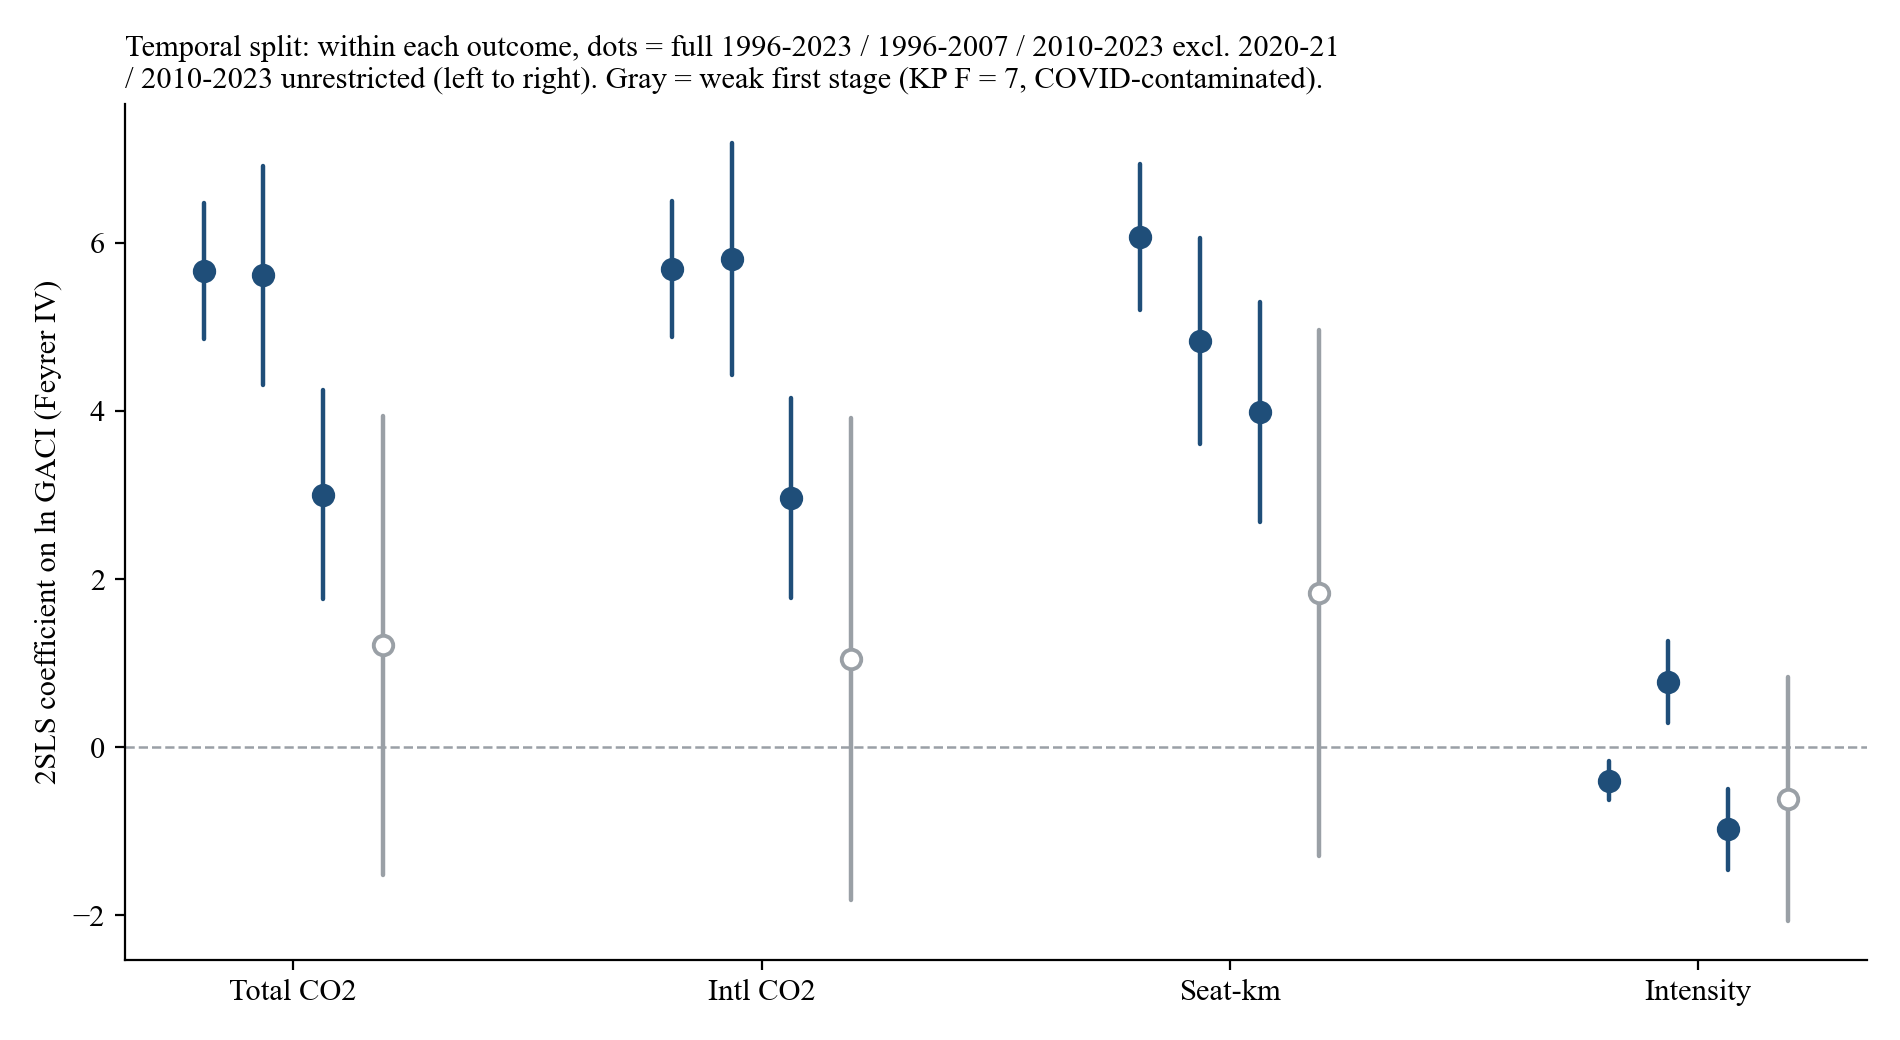
\includegraphics[width=0.92\textwidth]{CO2_temporal_coefplot.png}
\caption{Extended Data Fig.\ 1: Temporal split of the connectivity elasticity. Within each outcome, markers show the full sample, the network-expansion era (1996--2007), the mature-network era (2010--2023 excluding the COVID-19 years 2020--2021), and the unrestricted 2010--2023 sample from left to right; gray denotes the unrestricted later sample, whose first stage (KP $F=7$) is contaminated by the COVID collapse.}
\label{fig:temporal}
\end{figure}

\begin{figure}[htbp]
\centering
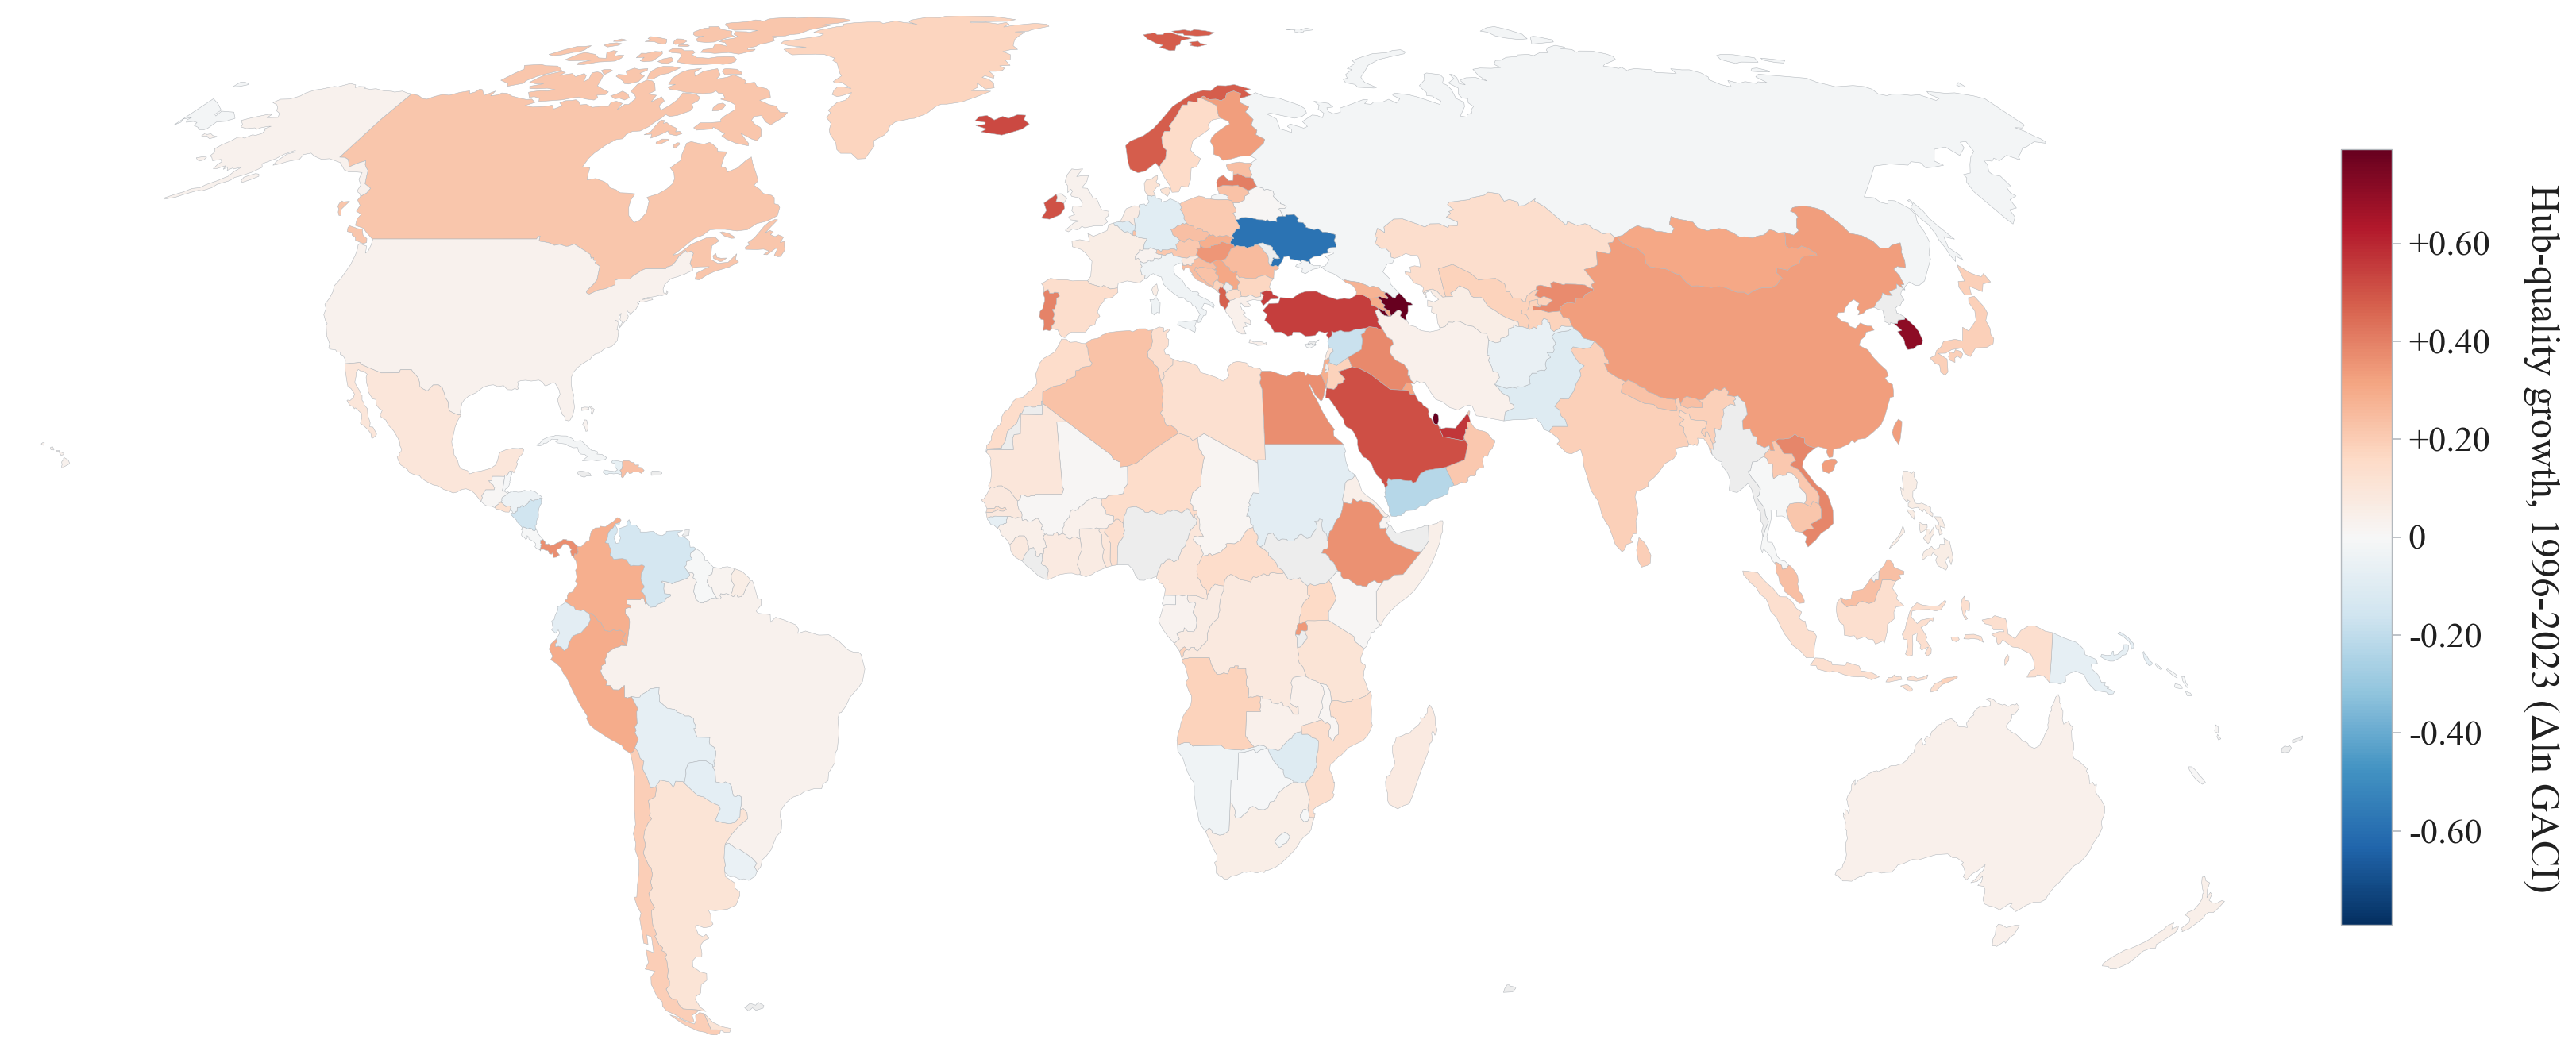
\includegraphics[width=0.92\textwidth]{CO2_map_dlngaci.png}
\caption{Extended Data Fig.\ 2: Change in log air connectivity (GACI, capacity-weighted mean), 1996--2023.}
\label{fig:dlngaci}
\end{figure}

\begin{figure}[htbp]
\centering
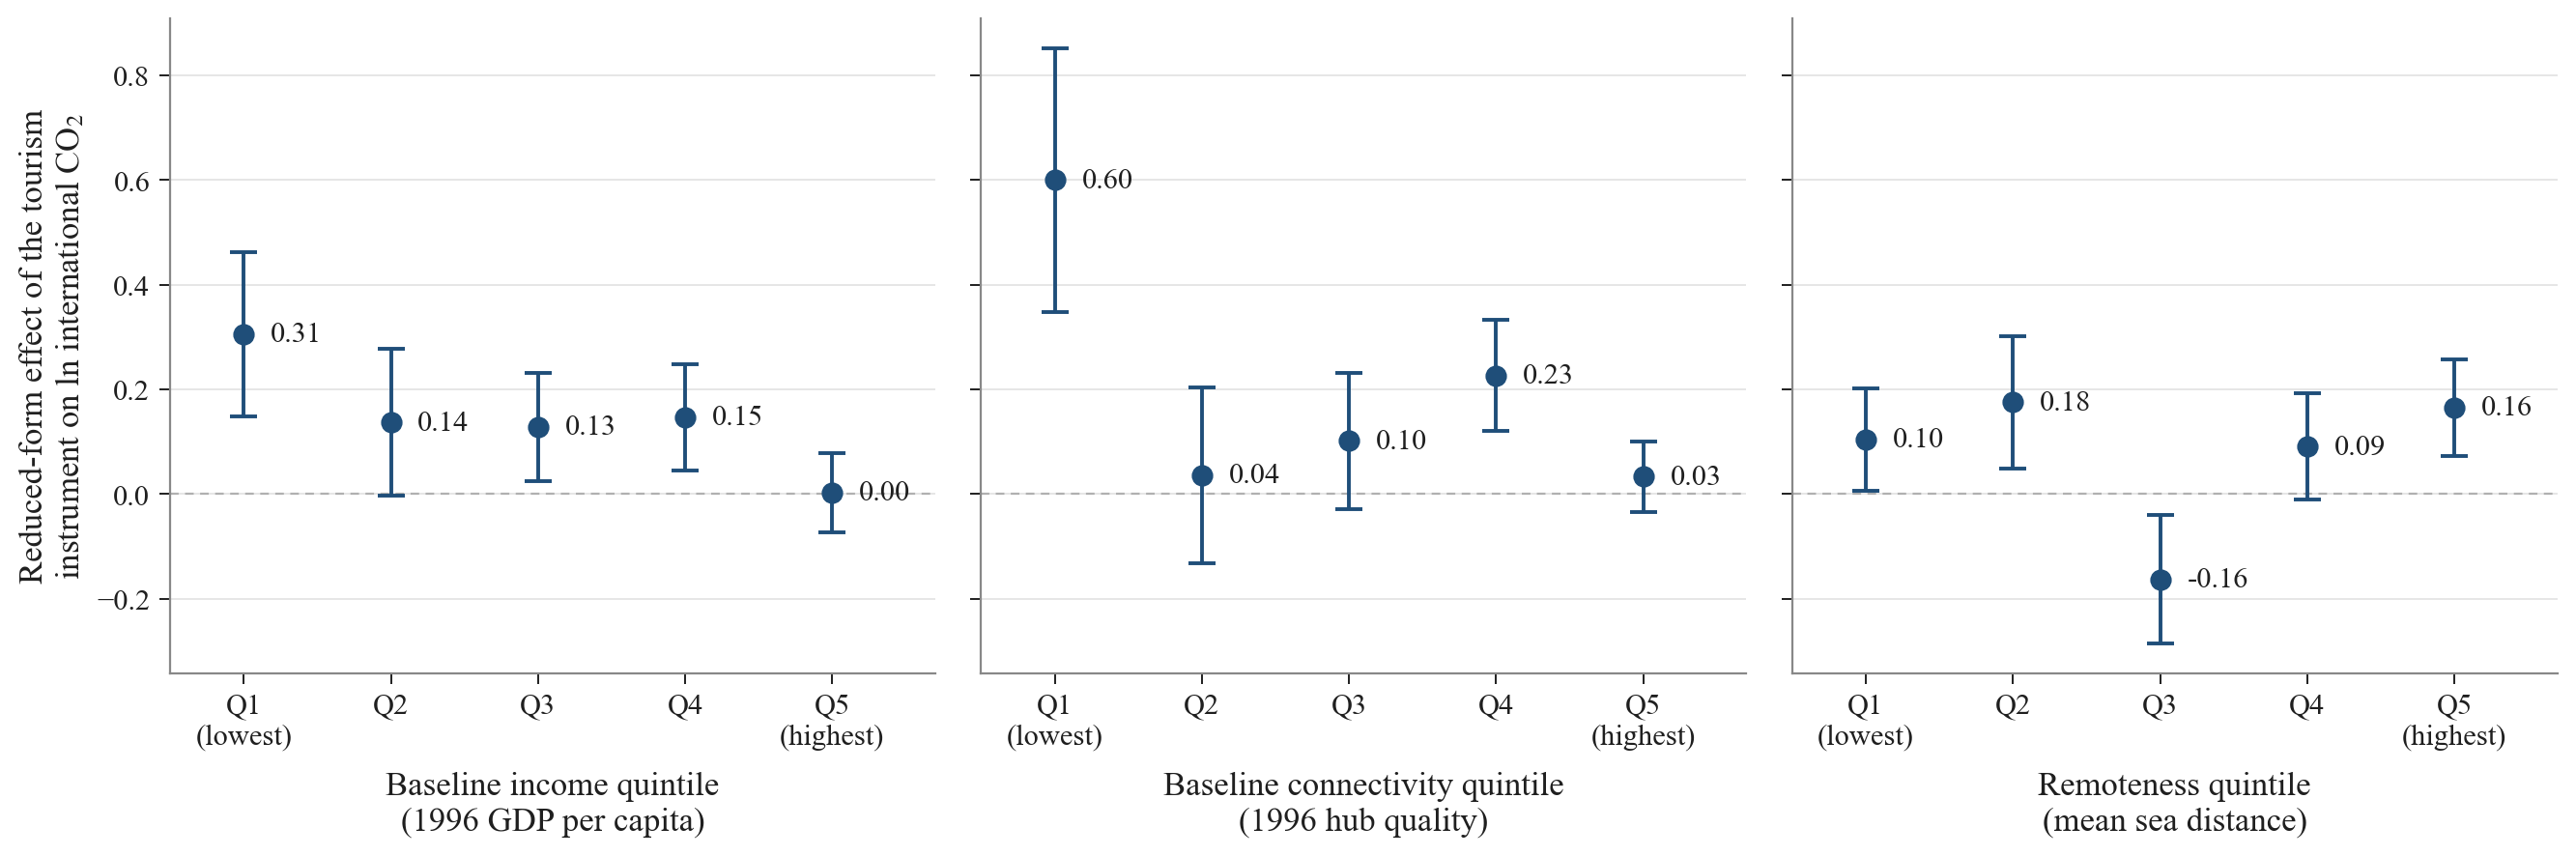
\includegraphics[width=0.92\textwidth]{CO2_rf_quintile.png}
\caption{Extended Data Fig.\ 3: Reduced-form quintile slopes under the tourism shifter: effects are concentrated in low-income, low-connectivity quintiles.}
\label{fig:rfquintile}
\end{figure}

\begin{figure}[htbp]
\centering
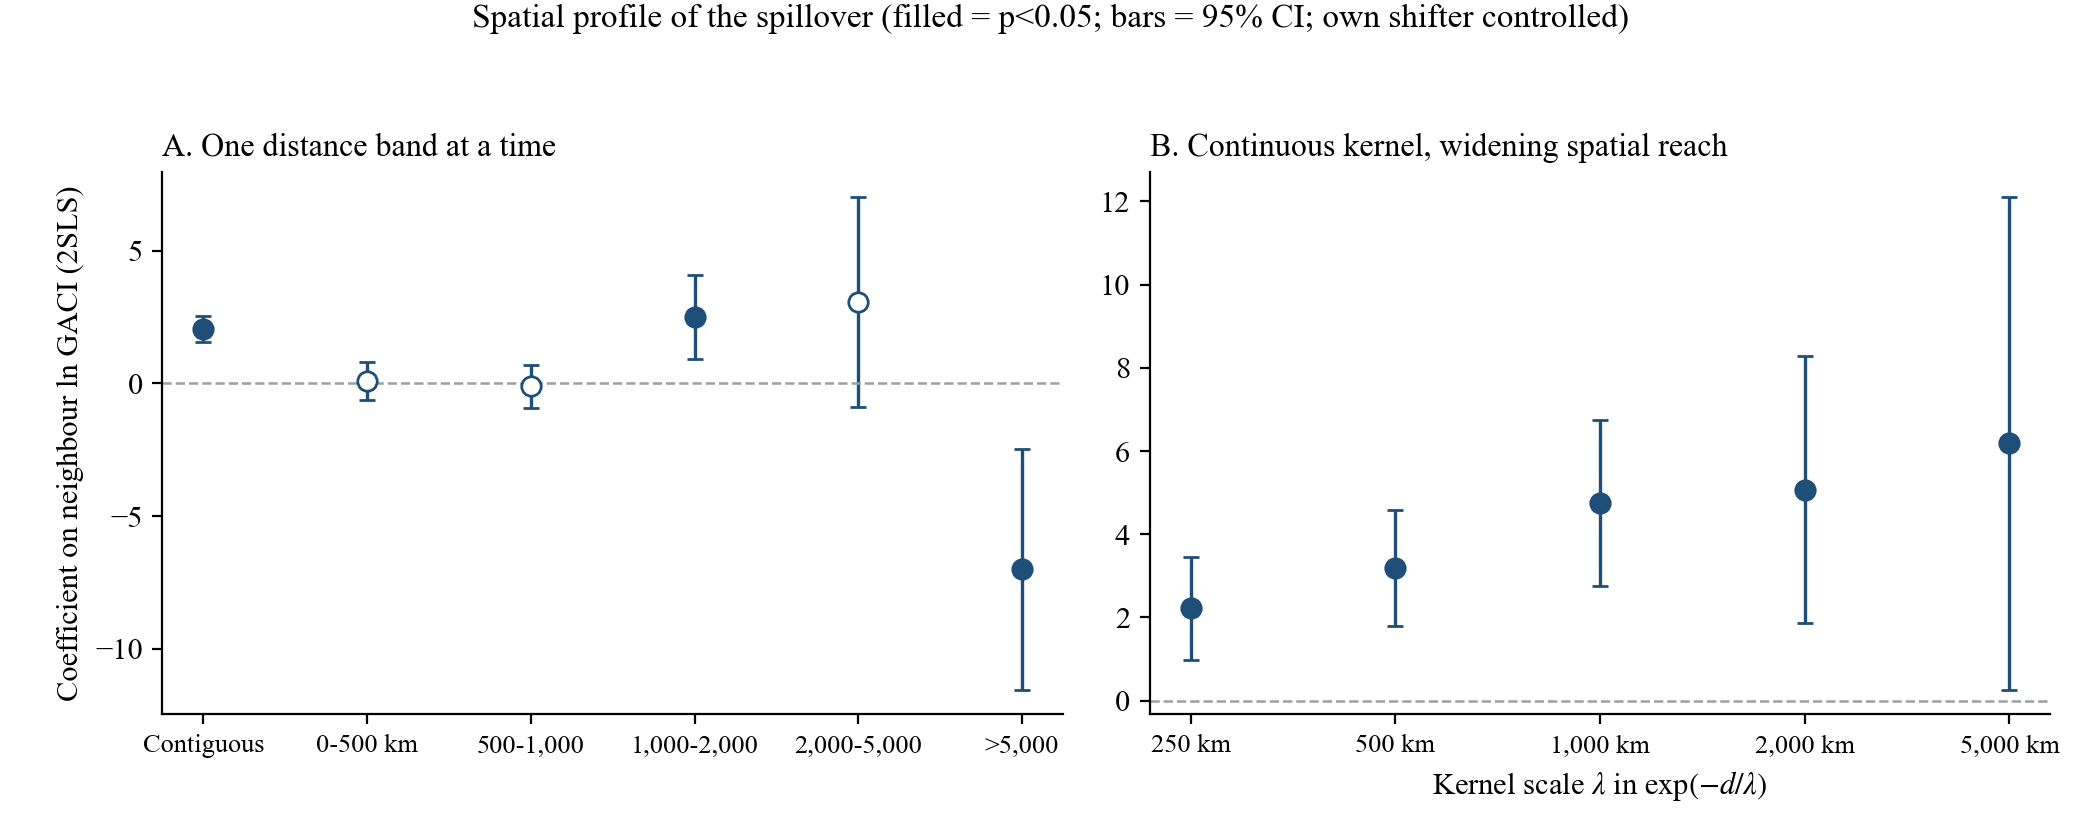
\includegraphics[width=0.92\textwidth]{CO2_spill_decay.png}
\caption{Extended Data Fig.\ 4: Spatial profile of the spillover. A, coefficient on neighbour connectivity when one distance band at a time defines the neighbours (contiguous countries, then bands of aviation-centroid distance); B, the same with an exponential kernel of widening scale. Neighbour connectivity is instrumented by the identically weighted shifter and the own shifter is controlled. The absence of a smooth decline and the significantly negative coefficient beyond 5{,}000 km indicate that wide exposures track global trends rather than a spatial spillover.}
\label{fig:spilldecay}
\end{figure}

\begin{figure}[htbp]
\centering
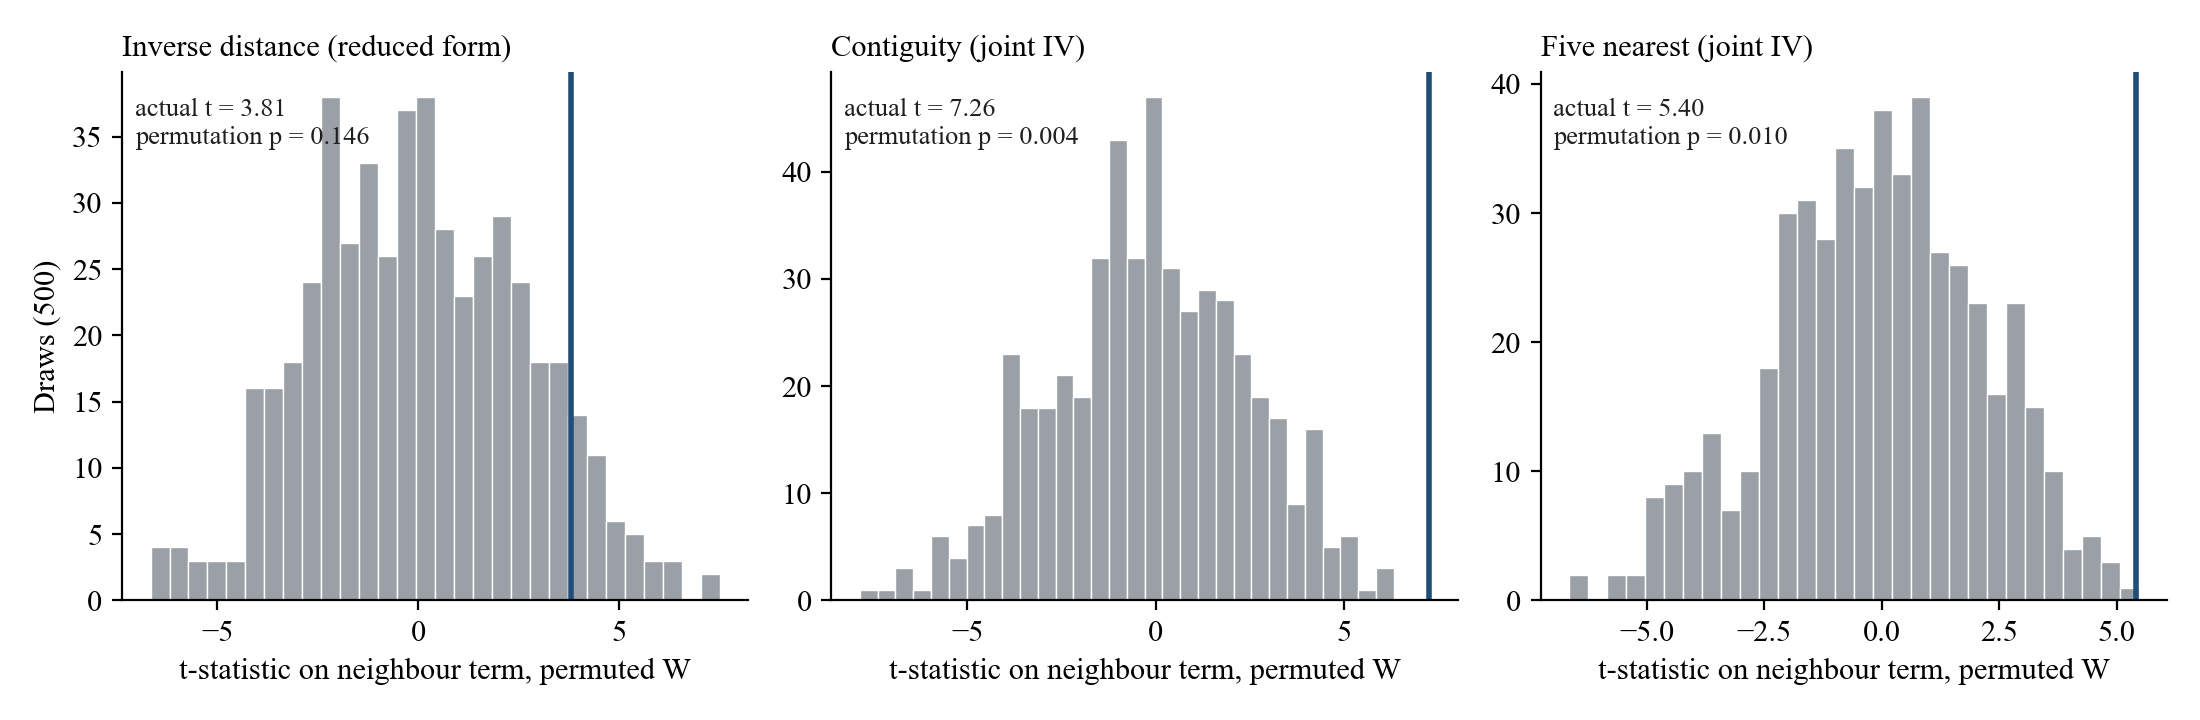
\includegraphics[width=0.92\textwidth]{CO2_spill_placebo.png}
\caption{Extended Data Fig.\ 5: Permutation placebo for the spillover. Distributions of the $t$-statistic on the neighbour term over 500 random relabellings of countries in the weight matrix, with the actual statistic in blue, for the inverse-distance reduced form and for the contiguity and five-nearest joint 2SLS specifications.}
\label{fig:spillplacebo}
\end{figure}

\begin{figure}[htbp]
\centering
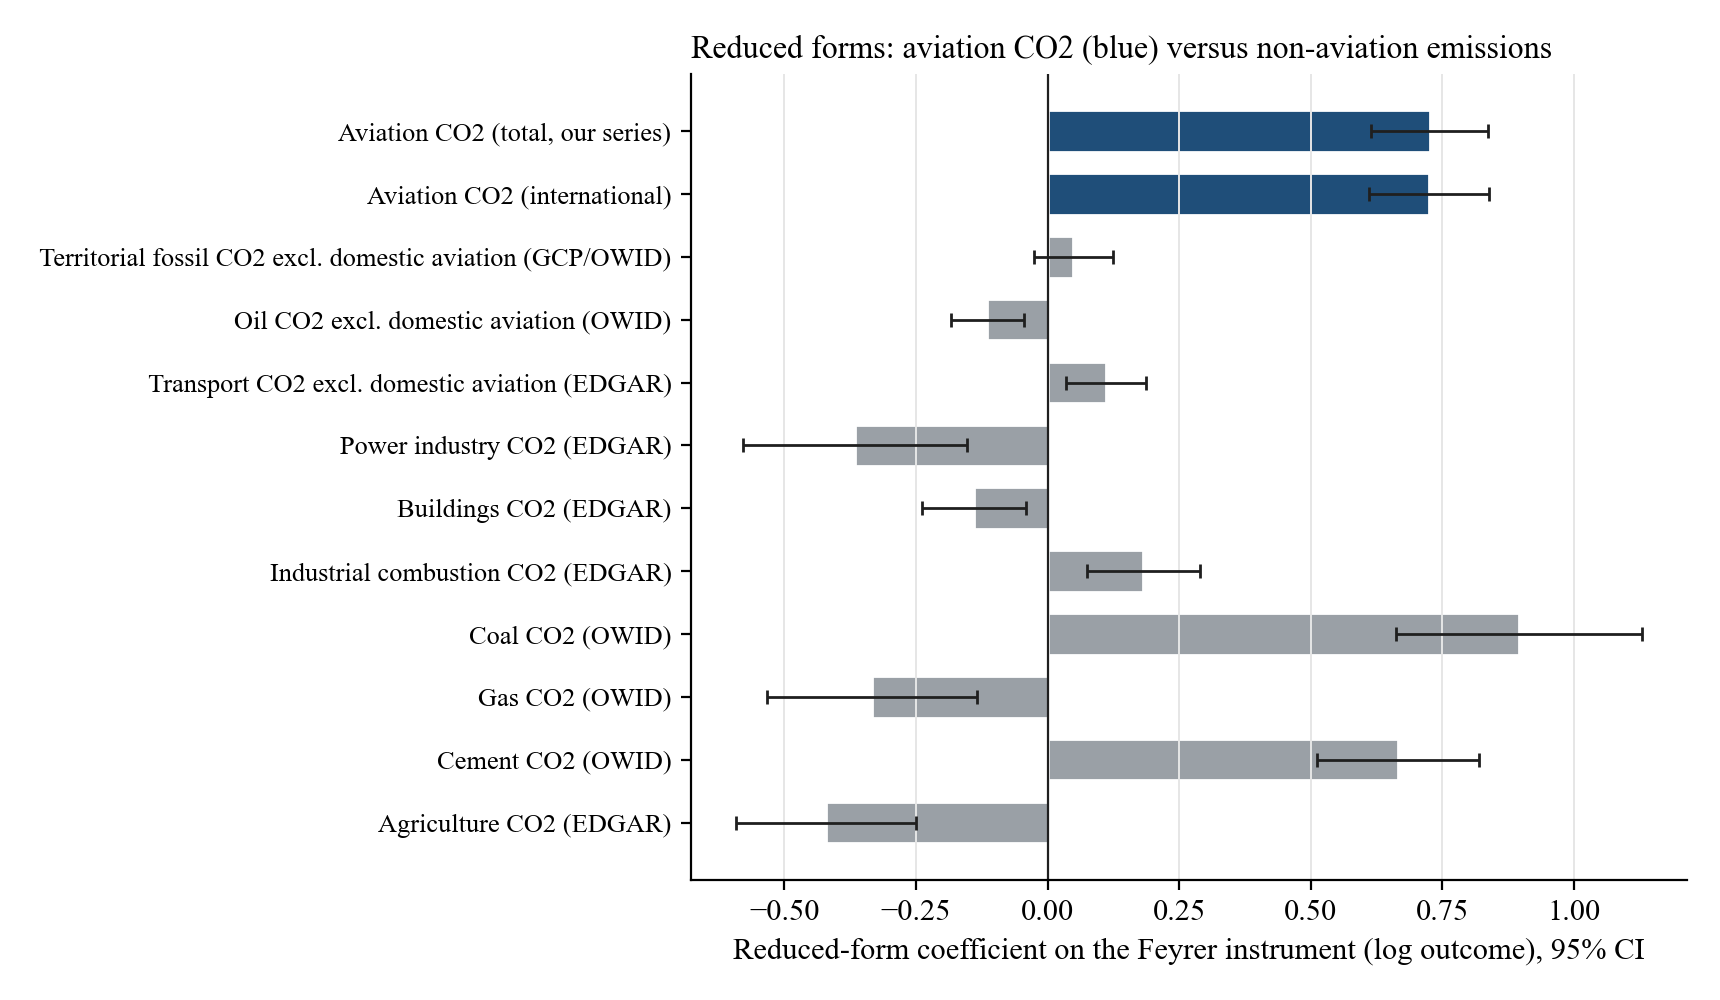
\includegraphics[width=0.92\textwidth]{CO2_placebo_rf.png}
\caption{Extended Data Fig.\ 6: Reduced forms of the Feyrer instrument on aviation CO$_2$ (blue) and on non-aviation emission series (grey), with 95 percent confidence intervals. Specification as in Table~\ref{tab:main}.}
\label{fig:placeborf}
\end{figure}

% Carbon-intensity-of-trade-gains map retained from the heritage pipeline
% (v1 framing, dropped from the main text per Sunbin; kept pending a
% decision).
\begin{figure}[htbp]
\centering
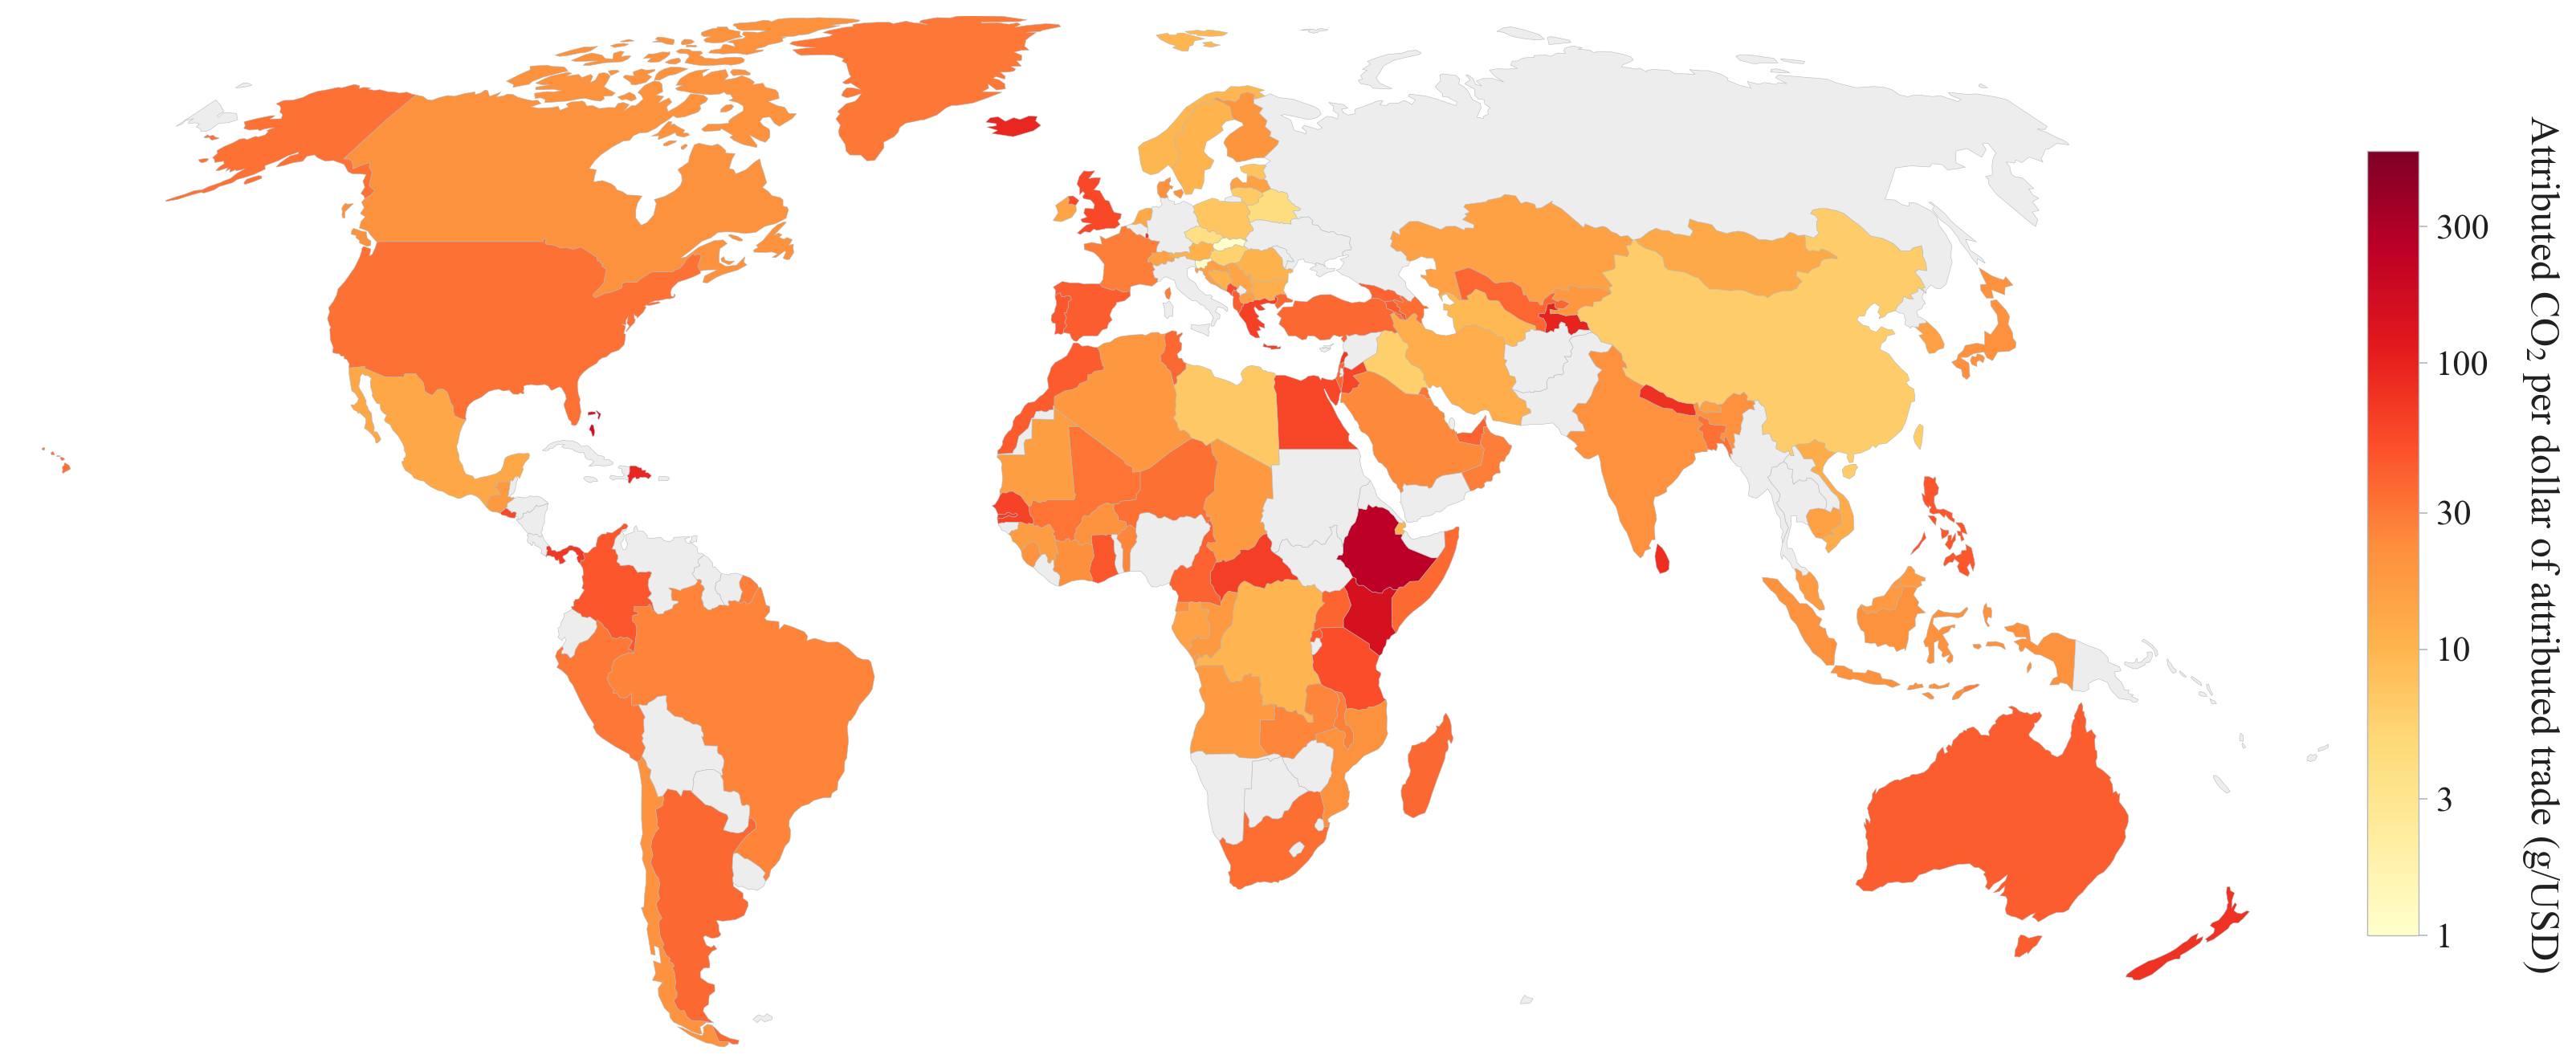
\includegraphics[width=0.92\textwidth]{CO2_map_carbonprice.png}
\caption{Extended Data Fig.\ 7: Carbon intensity of connectivity gains (g CO$_2$ per USD of trade gain; heritage-instrument pipeline).}
\label{fig:carbonprice}
\end{figure}

\clearpage
\section*{Supplementary Tables}

\begin{table}[htbp]
\centering
\begin{threeparttable}
\caption{Supplementary Table 1: Alternative instrument constructions, leads, overidentification and inference}
\label{tab:exclusion2}
\scriptsize
\begin{tabular}{lcccc}
\toprule
 & First-stage $\pi$ & 2SLS & KP $F$ & $N$ \\
\midrule
\multicolumn{5}{l}{\textit{Panel A. Technology series in the interaction (all $\times$ log 1996 air market access)}} \\
  World seat capacity (baseline) & 0.128$^{***}$ (0.010) & 5.67$^{***}$ (0.41) & 153.6 & 4,634 \\
  World flights & 0.121$^{***}$ (0.013) & 5.96$^{***}$ (0.55) & 90.7 & 4,121 \\
  World seat-km & 0.135$^{***}$ (0.011) & 5.90$^{***}$ (0.44) & 137.7 & 4,121 \\
  World sum of GACI & 0.123$^{***}$ (0.010) & 5.96$^{***}$ (0.40) & 161.4 & 4,121 \\
  World fuel-efficiency index (CO$_2$ per seat-km, inverted) & 0.145$^{***}$ (0.011) & 5.89$^{***}$ (0.39) & 172.7 & 4,121 \\
  Baseline geography recomputed ($\theta = 1$) & 0.127$^{***}$ (0.010) & 5.92$^{***}$ (0.42) & 159.3 & 4,623 \\
  Distance decay $\theta = 0.5$ & 0.273$^{***}$ (0.022) & 5.81$^{***}$ (0.42) & 151.5 & 4,623 \\
  Distance decay $\theta = 1.5$ & 0.073$^{***}$ (0.006) & 6.09$^{***}$ (0.45) & 146.4 & 4,623 \\
\midrule
\multicolumn{5}{l}{\textit{Panel B. Leads of the instrument (reduced form on log CO$_2$)}} \\
 & Current & Lead & & $N$ \\
  Three-year lead & 0.578$^{***}$ (0.063) & 0.413$^{***}$ (0.063) & & 4,078 \\
  Five-year lead & 0.724$^{***}$ (0.081) & 0.317$^{***}$ (0.069) & & 3,715 \\
\midrule
\multicolumn{5}{l}{\textit{Panel C. Overidentification and inference (2SLS on log CO$_2$)}} \\
 & 2SLS & s.e. & KP $F$ & $N$ \\
  Feyrer and tourism-heritage instruments jointly & 4.96$^{***}$ & (0.35) & 97.2 & 4,634 \\
  \quad Hansen $J$ (p-value) & \multicolumn{2}{c}{21.63 (0.000)} & & \\
  Tourism-heritage instrument alone & 1.17 & (0.83) & 19.7 & 4,634 \\
  Heteroskedasticity-robust (baseline) & 5.67$^{***}$ & (0.41) & 153.6 & 4,634 \\
  Clustered by country & 5.67$^{***}$ & (1.12) & 18.4 & 4,634 \\
  Two-way clustered (country, year) & 5.67$^{***}$ & (1.11) & 15.6 & 4,634 \\
\bottomrule
\end{tabular}
\begin{tablenotes}\scriptsize
\item Specification as in Table~\ref{tab:main}, column 1. Panel A replaces the world seat-capacity index by other min-max scaled world aviation series, or recomputes 1996 air market access with a different distance-decay exponent. Panel B enters the instrument dated $t+3$ or $t+5$ alongside its current value; because the technology index is a smooth global trend, the lead is mechanically collinear with the current value and this test is informative only about differential trends by geography. Panel C: the tourism-heritage instrument fails the size-by-cycle stress test (Methods) and is shown for reference; the Hansen test rejects equality of the two just-identified estimates. $^{***}$ $p<0.01$, $^{**}$ $p<0.05$, $^{*}$ $p<0.1$.
\end{tablenotes}
\end{threeparttable}
\end{table}

\begin{table}[htbp]
\centering
\begin{threeparttable}
\caption{Supplementary Table 2: Airport-level identification pilot with an airport Feyrer shifter}
\label{tab:airport_iv}
\scriptsize
\begin{tabular}{lccc}
\toprule
 & Coefficient & Partial / KP $F$ & $N$ \\
\midrule
\multicolumn{4}{l}{\textit{First stage: log airport GACI on $a_t \times$ log airport air market access 1996}} \\
  Baseline & -0.017 (0.027) & 0.4 & 76,366 \\
  \quad plus $a_t \times$ log 1996 seat-km & 0.022 (0.026) & 0.7 & 76,314 \\
  \quad plus $a_t \times$ log 1996 GACI & 0.016 (0.025) & 0.4 & 76,314 \\
\midrule
\multicolumn{4}{l}{\textit{2SLS (baseline instrument)}} \\
  log CO$_2$ & 2.42 (11.43) & 0.4 & 76,366 \\
  log seat-km & 9.92 (16.77) & 0.3 & 76,278 \\
  log CO$_2$/seat-km & 2.31 (6.95) & 0.3 & 76,278 \\
  International share & 1.99 (3.49) & 0.3 & 76,278 \\
\bottomrule
\end{tabular}
\begin{tablenotes}\scriptsize
\item Airport air market access is the population-weighted inverse distance from the airport to all foreign countries' aviation centroids in 1996 (own country excluded); $a_t$ is the world seat-capacity index of the country instrument. Airport and country-by-year fixed effects, standard errors clustered by airport. Within a country the shifter varies only through airports' relative location (mean within-country standard deviation of the log 1996 access term 0.04), and it has no first stage; the pilot is therefore not used and airport-level estimates are reported as within-country descriptive evidence.
\end{tablenotes}
\end{threeparttable}
\end{table}

\begin{table}[htbp]
\centering
\begin{threeparttable}
\caption{Supplementary Table 3: Aviation-accident instrument (Aviation Safety Network), pilot}
\label{tab:accident_iv}
\footnotesize
\begin{tabular}{lcccc}
\toprule
 & Bunker CO$_2$ & Intl.\ CO$_2$ & Intensity & KP $F$ \\
\midrule
  2SLS, Lagged fatal accidents & 6.20$^{**}$ (2.42) & 5.20$^{***}$ (2.00) & -1.10 (0.70) & 4.4 \\
  2SLS, Lagged accident deaths & 5.56$^{*}$ (3.02) & 3.73 (2.90) & -0.34 (1.02) & 2.0 \\
  2SLS, Lagged any-fatal-accident indicator & 7.08 (4.73) & 5.60 (4.21) & -1.32 (1.63) & 1.2 \\
  Feyrer and lagged fatal accidents jointly & 5.39$^{***}$ (0.42) & 5.36$^{***}$ (0.41) & -0.43$^{***}$ (0.13) & 66.8 \\
  \quad Hansen $J$ $p$-value & 0.70 & 0.93 & 0.21 & \\
  Feyrer and lagged accident deaths jointly & 5.38$^{***}$ (0.42) & 5.35$^{***}$ (0.41) & -0.42$^{***}$ (0.13) & 66.3 \\
  \quad Hansen $J$ $p$-value & 0.95 & 0.59 & 0.93 & \\
\bottomrule
\end{tabular}
\begin{tablenotes}[flushleft]
\footnotesize
\item Notes: Country-year accident counts and deaths from the Aviation Safety Network, lagged one year, as instruments for log GACI; specification otherwise as in Table~\ref{tab:main}. The accident instruments are weak (first-stage $F$ of 1 to 4) and are not used on their own; the joint specification with the Feyrer instrument is reported for the overidentification test. Robust standard errors in parentheses. $^{***}$, $^{**}$, $^{*}$: significance at 1, 5, and 10 percent.
\end{tablenotes}
\end{threeparttable}
\end{table}

\end{document}
